\chapter{Cubed-sphere finite-volume shallow-water model}
\label{chp-cs-swm}

Now that we have described how to solve the advection equation on the cubed-sphere in Chapter \ref{chp-cs-fv},
we are able to introduce the method of \citet{lin:1997} for solving the shallow-water equations (SWE) on the cubed-sphere.
In fact, this scheme considers the SWE in the vector invariant form, and therefore, 
the flux operators discussed in Chapter \ref{chp-cs-fv} are used to update the fluid depth,
as well as the time-averaged relative vorticity and kinetic energy fluxes.
This scheme first solves the SWE for a half time-step to obtain  C-grid covariant winds and 
then utilizes this new information to advance the  D-grid covariant winds for a full time step.
The C-grid half-step employs upwind flux operators, which are computationally inexpensive, 
while the D-grid uses PPM-based fluxes, providing higher accuracy. 
We note that other flux operators could be employed here, but the choice presented is what is utilized in FV3.

Although the advection equation on the sphere plays a crucial role in the development of dynamical cores by modeling the advection of scalar fields on the sphere, 
it does not capture important features present in the SWE on the sphere, 
such as the Coriolis effect, inertia-gravity waves, geostrophic adjustment, Rossby waves, among others. 
Therefore, SWE serve as an excellent benchmark for assessing dynamical cores in general,
as they are only two-dimensional but represent a complex geophysical model for atmosphere dynamics.
Furthermore, the 3D non-hydrostatic solver of FV3 utilizes a vertical Lagrangian coordinate system,
requiring the solution of the shallow-water equations on the Lagrangian surfaces \citep{lin:2004, harris:2021}.

The goal of this Chapter is to provide a detailed description of the SWE solver from \citet{lin:1997}.
Since this scheme uses advection operators to update the variables, 
we are going to incorporate the new advection scheme LT introduced in Chapter \ref{chp-cs-fv} and compare it with the PL advection scheme from \citet{putman:2007},
which is currently employed in FV3. 
Thus, we will extend the comparisons made in Chapter \ref{chp-cs-fv} to the context of the SWE.

This Chapter is outlined as follows:
In Section \ref{sec:sweq}, we introduce the SWE and some of its properties, and then we discuss
the C-grid and D-grid discretization proposed by \citet{lin:1997} in Section \ref{sw:fv3solver}.
Our modifications for their scheme are presented in Section \ref{sw-modf}.
Following that, in Section \ref{sec:numerical_results}, 
we present numerical results using classical tests from the literature. 
Finally, in Section \ref{sec:conclusions}, we provide concluding remarks.

\section{The shallow-water equations on the sphere}
\label{sec:sweq}
In this Section, we introduce the shallow-water equations (SWE) on the sphere using a cubed-sphere mapping 
(equi-edge or equiangular) as discussed in Section \ref{sec-cs-grids}.
All the notation from Sections \ref{cs-mappings} and \ref{sec-cs-grids} is utilized here.
For simplicity, we omit the dependence on $p$ since it does not affect the description across cube faces.
Additionally, we assume that the ghost cells are filled using the duo-grid interpolation scheme outlined in Sections \ref{cs-interp} and \ref{cs-wind-interp}.
The shallow-water equations (SWE) are a set of hyperbolic partial differential equations describing how the fluid depth, 
denoted by $h$, and the wind $\boldsymbol{u}$ evolve with time.
Since the cubed-sphere system is non-orthogonal, the SWEs will feature the covariant winds $\mathfrak{U}, \mathfrak{V}$ and
contravariant winds $\mathfrak{u}, \mathfrak{v}$, as discussed in Section \ref{cs-tgvectors}.
The SWE on the a cubed-sphere panel are expressed as in its vector invariant form as \citep{rancic:1996, nair:2005b}:
\begin{align}
	\label{2d-sweq-h}
	{\partial_t (\sqrt{\mathfrak{g}} {h})}(x, y, t) &= -
	[{\partial_x (\mathfrak{u}\sqrt{\mathfrak{g}}{h}}
	+ {\partial_y (\mathfrak{v}\sqrt{\mathfrak{g}}{h})}](x, y, t), \\
	\label{2d-sweq-u}
	{\partial_t \mathfrak{U}}(x, y, t)&=
	-[\partial_x K - \mathfrak{v}\sqrt{\mathfrak{g}}\xi +\partial_x \Phi] (x, y, t), \\
	\label{2d-sweq-v}
	{\partial_t \mathfrak{V}}(x, y, t)&=
	-[\partial_y K + \mathfrak{u}\sqrt{\mathfrak{g}}\xi + \partial_y \Phi](x, y, t), 
\end{align}
$\Phi = g(h+b)$ is the geopotential, $g$ is the gravity, $b$ is the bottom topography,
\begin{equation}
	\label{ke-eq}
	K = \frac{\mathfrak{u}\mathfrak{U}+\mathfrak{v}\mathfrak{V}}{2},
\end{equation}
is the kinetic energy,
\begin{equation}
	\label{vort-eq}
	\xi = f+ \zeta,
\end{equation}
is the absolute vorticity, where
\begin{equation}
	\label{coriolis-eq}
	f  = 2 \Omega \sin{\phi},
\end{equation}
is the Coriolis parameter,
$\phi$ is the latitude, $\Omega = 7.2921 \times 10^{-5}$ is the Earth rotation speed, and
\begin{equation}
	\label{vort2-eq}
	\zeta = \frac{1}{\sqrt{\mathfrak{g}}}(\partial_x \mathfrak{V} - \partial_y\mathfrak{U}),
\end{equation}
is the relative vorticity.

%\section{Elementary properties of the SWE}
%\label{sec:sweq-prop}
Now, let us describe some elementary properties of the SWE.
By taking $\partial_y$ in Equation \eqref{2d-sweq-u} and $\partial_x$ in Equation \eqref{2d-sweq-v} and
subtracting the obtained results, we get that the absolute vorticity satisfies:
\begin{align}
	\label{absvort-eq}
	{\partial_t (\sqrt{\mathfrak{g}} {\xi})}(x,y,t) & = 
	-[{\partial_x (\mathfrak{u}\sqrt{\mathfrak{g}}{\xi}})
	+ {\partial_y (\mathfrak{v}\sqrt{\mathfrak{g}}{\xi}})](x,y,t).
\end{align}
One can also easily show (as described in Section \ref{chp-cs-adv}) that the total mass of $h$ and $\zeta$ is preserved.

By replacing Equations \eqref{contra-uv} and \eqref{covari-uv} in Equation \eqref{ke-eq}, 
it follows that the kinetic energy may be rewritten in terms of the normalized contravariant and covariant wind components as:
\begin{equation}
	\label{ke-eq2}
	K = \frac{{u}{U}+{v}{V}}{2}.
\end{equation}
Recall that the normalized contravariant and covariant wind components
are given by Equation \eqref{contra-uv} and Equation \eqref{norm-covariant-u}, respectively.

The total energy is defined as:
\begin{equation}
	\label{energy}
	E = g\frac{h^2}{2} + gb + hK.
\end{equation}
One can deduce an equation for the time evolution of the total energy (see, for example, \citet{ringler:2010}) 
and observe that its integral over the sphere is preserved; that is, the total energy is conserved.
%The total entrosphy is defined as
%\begin{equation}
%	\label{enstrophy}
%	E = g\frac{h^2}{2} + gb + hK,
%\end{equation}

\subsection{Momentum equation discretization}
The continuity equation \eqref{2d-sweq-h} has the exact same form as the advection equation when written in its conservative form.
Therefore, this equation can be solved on the A-grid using C-grid contravariant winds, as explored in Chapters \ref{chp-2d-fv} and \ref{chp-cs-fv}.
This is how the continuity equation is solved in FV3.
As we shall see later, this equation is solved twice: 
once using the 2D upwind flux and another using the dimension-splitting method from Chapter \ref{chp-cs-fv} with PPM.

Therefore, we need to describe how we can solve the momentum equations \eqref{2d-sweq-u} and \eqref{2d-sweq-v}. 
The method of \citet{lin:1997} employs two types of approaches on their shallow-water solver: one using a C-grid wind and the other using a D-grid wind.
The C-grid method serves as an intermediate step utilized by the D-grid method.
Our goal now is to describe a general discretization of the momentum equations for the C-grid and D-grid winds.
The full description of the C-grid and D-grid solvers proposed by 
\citet{lin:1997} will be provided in Sections \ref{csw-grid} and \ref{dsw-grid}, respectively.

\subsubsection{D-grid discretization of the momentum equation }
We introduce the following average operators for the covariant wind components in $x$ and $y$ directions, respectively:
\begin{align}
	\label{2d-sweq-int_u}
	\overline{\mathfrak{U}^x_{i,j+\frac{1}{2}}}(t)&= \frac{1}{\Delta x} \int_{x_{i-\frac{1}{2}}}^{x_{i+\frac{1}{2}}} \mathfrak{U}(x, y_{j+\frac{1}{2}}, t) \,dx , \quad i=1,\ldots,N,j=0,\ldots, N,\\
	\label{2d-sweq-int_v}
	\overline{\mathfrak{V}^y_{i+\frac{1}{2},j}}(t)&= \frac{1}{\Delta y} \int_{y_{j-\frac{1}{2}}}^{y_{j+\frac{1}{2}}} \mathfrak{V}(x_{i+\frac{1}{2}}, y, t) \,dy,  \quad i=0,\ldots,N,j=1,\ldots, N.
\end{align}
We shall also use the notation $q_{ij}(t) = q(x_i,y_j,t)$ for any function $q$ and integer or half-integer indices $i$ and $j$.
We also use the centered difference notations $\delta _i q_{ij}(t) =q_{i+\frac{1}{2},j}(t) -q_{i-\frac{1}{2},j}(t)$ and 
$\delta _j q_{ij}(t) = q_{i,j+\frac{1}{2}}(t) -q_{i,j-\frac{1}{2}}(t)$ for any integer or half-integer indices $i$ and $j$.

By integrating Equation \eqref{2d-sweq-u} with respect to $x$ on $[x_{i-\frac{1}{2}},x_{i+\frac{1}{2}}]$ and Equation \eqref{2d-sweq-v} with respect to $y$ on $[y_{j-\frac{1}{2}},y_{j+\frac{1}{2}}]$, we get the following equations:
\begin{align}
	\label{2d-sweq-int_equ}
	\frac{d}{dt}\overline{\mathfrak{U}^x_{i,j+\frac{1}{2}}}
	(t)&= -\frac{\delta_i K_{i,j+\frac{1}{2}}(t)}{\Delta x}-\frac{\delta_i \Phi_{i,j+\frac{1}{2}}(t)}{\Delta x} + 
	\frac{1}{\Delta x}
	\int_{x_{i-\frac{1}{2}}}^{x_{i+\frac{1}{2}}}
	(\mathfrak{v}\sqrt{\mathfrak{g}}\xi)(x_i, y_{j+\frac{1}{2}}, t) \,dx, \\
	\label{2d-sweq-int_eqv}
	\frac{d}{dt} \overline{\mathfrak{V}^y_{i+\frac{1}{2},j}}(t)&= -\frac{\delta_j K_{i+\frac{1}{2},j}(t)}{\Delta y}-
	\frac{\delta_j \Phi_{i+\frac{1}{2},j}(t)}{\Delta y}
	- \frac{1}{\Delta y}
	\int_{y_{j-\frac{1}{2}}}^{y_{j+\frac{1}{2}}} 
	(\mathfrak{u}\sqrt{\mathfrak{g}}\xi)(x_{i+\frac{1}{2}}, y, t) \,dy.
\end{align}
Integrating Equations \eqref{2d-sweq-int_equ} and \eqref{2d-sweq-int_eqv} on time over $[t^n,t^{n+1}]$, we obtain:
\begin{align}
	\label{2d-sweq-int_equt}
	\overline{\mathfrak{U}^x_{i,j+\frac{1}{2}}}(t^{n+1})&=
	\overline{\mathfrak{U}^x_{i,j+\frac{1}{2}}}(t^{n}) -
	\int_{t_{n}}^{t_{n+1}}\bigg[
	\frac{\delta_i K_{i,j+\frac{1}{2}}(t)}{\Delta x}
	+\frac{\delta_i \Phi_{i,j+\frac{1}{2}}(t)}{\Delta x} - \bigg(
	\int_{x_{i-\frac{1}{2}}}^{x_{i+\frac{1}{2}}}
	\frac{(\mathfrak{v}\sqrt{\mathfrak{g}}\xi)(x_i, y_{j+\frac{1}{2}}, t)}{\Delta x}
	\,dx \bigg)\bigg]
	\,dt ,\\
	\label{2d-sweq-int_eqvt}
	\overline{\mathfrak{V}^y_{i+\frac{1}{2},j}}(t^{n+1})&=
	\overline{\mathfrak{V}^y_{i+\frac{1}{2},j}}(t^{n}) -
	\int_{t_{n}}^{t_{n+1}}\bigg[
	\frac{\delta_j K_{i+\frac{1}{2},j}(t)}{\Delta y}+\frac{\delta_j\Phi_{i+\frac{1}{2},j}(t)}{\Delta y}+ \bigg(
	\int_{y_{j-\frac{1}{2}}}^{y_{j+\frac{1}{2}}} 
	\frac{(\mathfrak{u}\sqrt{\mathfrak{g}}\xi)(x_{i+\frac{1}{2}}, y, t)}{\Delta y}
	\,dy \bigg)\bigg]\,dt .
\end{align}
Using the midpoint rule and using the normalized covariant winds in Equations \eqref{2d-sweq-int_equt} and \eqref{2d-sweq-int_eqvt}, we derive a general scheme
to update the normalized D-grid covariant winds:
\begin{align}
	\label{2d-sweq-dscheme-u}
	{U}_{i,j+\frac{1}{2}}^{n+1}&=
	{U}_{i,j+\frac{1}{2}}^{n} - \bigg(
	\frac{\delta_i K_{i,j+\frac{1}{2}}^n}{\hat{\delta} x_{i,j+\frac{1}{2}}}
	+\frac{\delta_i \Phi_{i,j+\frac{1}{2}}^n}{\hat{\delta} x_{i,j+\frac{1}{2}}}
	- \frac{G_{i,j+\frac{1}{2}}}{{\hat{\delta} x_{i,j+\frac{1}{2}}}}[\xi, v^n]\bigg)
	,\\
	\label{2d-sweq-dscheme-v}
	{V}_{i+\frac{1}{2},j}^{n+1}&=
	{V}_{i+\frac{1}{2},j}^{n} - \bigg(
	\frac{\delta_j K_{i+\frac{1}{2},j}}{\hat{\delta} y_{i+\frac{1}{2},j}}+
	\frac{\delta_j \Phi_{{i+\frac{1}{2}},j}^n}{\hat{\delta} y_{i+\frac{1}{2},j}}
	+ \frac{F_{i+\frac{1}{2},j}[\xi, u^n]}{\hat{\delta} y_{i+\frac{1}{2},j}} \bigg).
\end{align}
Then, this schemes requires an approximation of the time-averaged kinetic energy at the B-grid:
\begin{equation}
	\label{ke-bgrid}
	K_{i+\frac{1}{2},j+\frac{1}{2}}^n \approx \frac{1}{2}\bigg[
	\int_{t_{n}}^{t_{n+1}} ({u}{U})(x_{i+\frac{1}{2}}, y_{j+\frac{1}{2}}, t) \,dt +
	\int_{t_{n}}^{t_{n+1}} ({v}{V})(x_{i+\frac{1}{2}}, y_{j+\frac{1}{2}}, t) \,dt\bigg],
\end{equation}
and an approximation of the time-averaged geopotential on B-grid:
\begin{equation}
	\label{geop-bgrid}
	\Phi_{i+\frac{1}{2},j+\frac{1}{2}}^n \approx
	\int_{t_{n}}^{t_{n+1}} \Phi
	(x_{i+\frac{1}{2}}, y_{j+\frac{1}{2}}, t) \,dt,
\end{equation}
The terms should $F_{i+\frac{1}{2},j}[\xi^{n}, u^n]$ and $G_{i,j+\frac{1}{2}}[\xi^{n}, v^n] $ should approximate the time-averaged absolute vorticity fluxes:
\begin{align}
	F_{i+\frac{1}{2},j}[\xi^{n}, u^n] \approx
	\int_{t^n}^{t^{n+1}} 
	\int_{y_{j-\frac{1}{2}}}^{y_{j+\frac{1}{2}}} 
	{(\mathfrak{u}\sqrt{\mathfrak{g}}\xi)(x_{i+\frac{1}{2}}, y, t)}
	\,dy \,dt \\
	G_{i,j+\frac{1}{2}}[\xi^{n}, v^n] \approx
	\int_{t^n}^{t^{n+1}} 
    \int_{x_{i-\frac{1}{2}}}^{x_{i+\frac{1}{2}}} 
    {(\mathfrak{v}\sqrt{\mathfrak{g}}\xi)(x, y_{j+\frac{1}{2}}, t)}
    \,dx \,dt.
\end{align}
Notice that since $\xi$ satisfies the advection equation \eqref{absvort-eq}, 
these integrals may be approximated using finite-volume fluxes assuming that $\xi$ may be advected on the A-grid.
Indeed, this is possible because, as we shall see soon, the  D-grid covariant wind facilitates the estimation of $\xi$ on the A-grid by using centered finite differences.
All these approximations needed for the D-grid scheme are described in Section \ref{dsw-grid}.


\subsubsection{C-grid discretization of the momentum equation }
Similar to the derivation of the  D-grid covariant wind scheme, we may deduce the following C-grid covariant wind scheme for a half-time step:
\begin{align}
	\label{2d-sweq-cscheme-u}
	{U}_{i+\frac{1}{2},j}^{n+1}&=
	{U}_{i+\frac{1}{2},j}^{n} - \bigg(
	\frac{\delta_i K_{i+\frac{1}{2},j}^n}{\hat{\delta} x_{i+\frac{1}{2},j}}
	+\frac{\delta_i \Phi_{i+\frac{1}{2},j}^n}{\hat{\delta} x_{i+\frac{1}{2},j}} -
    \frac{G_{i+\frac{1}{2},j}[\xi^{n}, v^n]}{\hat{\delta} x_{i+\frac{1}{2},j}}\bigg),\\
	\label{2d-sweq-cscheme-v}
	{V}_{i,j+\frac{1}{2}}^{n+1}&=
	{V}_{i,j+\frac{1}{2}}^{n} - \bigg(
	\frac{\delta_j K_{i,j+\frac{1}{2}}}{\hat{\delta} y_{i,j+\frac{1}{2}}}+
	\frac{\delta_j \Phi_{{i,j+\frac{1}{2}}}^n}{\hat{\delta} y_{i,j+\frac{1}{2}}}
	+
   \frac{F_{i,j+\frac{1}{2}}[\xi, u^n]}{\hat{\delta} y_{i,j+\frac{1}{2}}}\bigg).
\end{align}
Then, this schemes requires an approximation of the time-averaged kinetic energy at the A-grid
\begin{equation}
	\label{ke-agrid}
	K_{ij}^n \approx \frac{1}{2}\bigg[
	\int_{t_{n}}^{t_{n+\frac{1}{2}}} ({u}{U})
	(x_{i}, y_{j}, t) \,dt +
	\int_{t_{n}}^{t_{n+\frac{1}{2}}} ({v}{V})
	(x_{i}, y_{j}, t) \,dt\bigg],
\end{equation}
and an approximation of the time-averaged geopotential on A-grid points:
\begin{equation}
	\label{geop-agrid}
	\Phi_{ij}^n \approx
	\int_{t_{n}}^{t_{n+\frac{1}{2}}} \Phi
	(x_{i}, y_{j}, t) \,dt.
\end{equation}
The terms should $F_{i,j+\frac{1}{2}}[\xi^{n}, u^n]$ and $G_{i+\frac{1}{2},j}[\xi^{n}, v^n] $ should approximate the time-averaged absolute vorticity fluxes:
\begin{align}
	F_{i,j+\frac{1}{2}}[\xi^{n}, u^n] \approx
	\int_{t^n}^{t^{n+\frac{1}{2}}} 
	\int_{y_{j}}^{y_{j+1}} 
	{(\mathfrak{u}\sqrt{\mathfrak{g}}\xi)(x_{i}, y, t)}
	\,dy \,dt \\
	G_{i+\frac{1}{2},j}[\xi^{n}, v^n] \approx
	\int_{t^n}^{t^{n+\frac{1}{2}}} 
	\int_{x_{i}}^{x_{i+1}} 
	{(\mathfrak{v}\sqrt{\mathfrak{g}}\xi)(x, y_{j}, t)}
	\,dx \,dt.
\end{align}
Once again, since $\xi$ satisfies the advection equation \eqref{absvort-eq}, 
these integrals may be approximated using finite-volume fluxes assuming that $\xi$ may be advected on the B-grid.
Indeed, this is possible because, as we shall see soon, the C-grid covariant wind facilitates the estimation of $\xi$ on the B-grid by using centered finite differences.
All these approximations are described in Section \ref{csw-grid}.

\section{The FV3 shallow-water solver}
\label{sw:fv3solver}
This Section is dedicated to presenting all the details of the shallow-water solver proposed by \citet{lin:1997} on the cubed-sphere. 
The C-grid intermediate step is described in Section \ref{csw-grid}, while the D-grid step is detailed in Section \ref{dsw-grid}.

\subsection{C-grid intermediate step}
\label{csw-grid}
The C-grid intermediate step serves to provide the  C-grid contravariant winds centered at time 
${u}^{n+\frac{1}{2}}_{i+\frac{1}{2},j}$ and ${v}^{n+\frac{1}{2}}_{i,j+\frac{1}{2}}$
that are required by the advection fluxes when using PPM, as discussed in Chapters \ref{chp-2d-fv} and \ref{chp-cs-fv}. 
One could utilize second-order extrapolation to obtain these centered at time C-grid winds, using two time levels, namely:
\begin{align}
{u}^{n+\frac{1}{2}}_{i+\frac{1}{2},j} = \frac{3}{2} {u}^{n}_{i,j+\frac{1}{2}} - \frac{1}{2} {u}^{n-1}_{i,j+\frac{1}{2}}, \\
{v}^{n+\frac{1}{2}}_{i,j+\frac{1}{2}} = \frac{3}{2} {v}^{n}_{i,j+\frac{1}{2}} - \frac{1}{2} {v}^{n-1}_{i,j+\frac{1}{2}}.
\end{align}
This approach is very popular in Semi-Lagrangian methods.
However, as pointed out by \citet{lin:1997}, this extrapolation introduces 2$\Delta x$ numerical noise, which may degrade the solution in presence
of sharp bottom topography. 
Therefore, \citet{lin:1997} proposes solving the SWE on a C-grid for a half-time step to provide the winds centered at time $n+\frac{1}{2}$. 
To make this half-time step cheaper, upwind fluxes are going to be used.
Our goal now is to describe the details of this C-grid wind solver.
We are going to describe everything that is needed to advance the 
C-grid winds given by Equations \eqref{2d-sweq-cscheme-u} and \eqref{2d-sweq-cscheme-v}.

\subsubsection{Wind interpolation}
We are given the D-grid covariant wind,
that is, we have $U_{i,j+\frac{1}{2}}^n$ for $i=0,\ldots,N$, $j=1,\ldots,N$, 
and $V_{i+\frac{1}{2},j}^n$ $j=0,\ldots,N$, $i=1,\ldots,N$.
We may then use the duo-grid interpolation (Section \ref{cs-wind-interp}) to get the values on the duo-grid.
After that, we have all the values 
$U_{i,j+\frac{1}{2}}^n$ for $i=0,\ldots,N+\nu$, $j=1,\ldots,N+\nu$, 
and $V_{i+\frac{1}{2},j}^n$ $j=0,\ldots,N+\nu$, $i=1,\ldots,N+\nu$.

We define the average operator in the $x$ direction as:
\begin{align}
	\label{av-x}
	\overline{q_{ij}}^x =
	\begin{cases}
	0.5(q_{i+\frac{1}{2},j}+q_{i-\frac{1}{2},j}), 
	\quad &
	\text{if } i=-\nu+1 \text{ or } i=N+\nu,\\
	\frac{9}{16}(q_{i+\frac{1}{2},j}+q_{i-\frac{1}{2},j}) - \frac{1}{16}(q_{i+\frac{3}{2},j}+q_{i-\frac{3}{2},j}), 
	\quad &
	\text{otherwise},\\
\end{cases}
\end{align}
for any integer $i$ and integer or half integer $j$, and
\begin{align}
	\label{av-xx}
	\overline{q_{i+\frac{1}{2},j}}^x =
	\begin{cases}
		0.5(q_{i+1,j}+q_{ij}), 
		\quad &
		\text{if } i=-\nu+1 \text{ or } i=N+\nu,\\
		\frac{9}{16}(q_{i+1,j}+q_{ij}) - \frac{1}{16}(q_{i+2,j}+q_{i-1,j}), 
		\quad &
		\text{otherwise},\\
	\end{cases}
\end{align}
for any integer $i$ and integer or half integer $j$.
The average operator $\overline{q_{ij}}^y$ in the $y$ direction is defined analogously.


We may interpolate the normalized covariant component $U$ from the D-grid to A-grid by using the average in the $y$ direction:
\begin{align}
	\label{d2a-u}
	 U_{ij}^n &= \overline{U_{ij}^n}^y,%\frac{U_{i,j+\frac{1}{2}}^n + U_{i,j-\frac{1}{2}}^n}{2},
\end{align}
for $i=-\nu+1,\ldots,N+\nu$, $j=-\nu+1,\ldots,N+\nu$, and similarly to the $V$ component:
\begin{align}
	\label{d2a-v}
	V_{ij}^n &=\overline{V_{ij}^n}^x,
\end{align}
for $j=-\nu+1,\ldots,N+\nu$, $i=-\nu+1,\ldots,N+\nu$.

Moreover, using the A-grid covariant wind, we may convert the wind from 
covariant to contravariant on the A-grid representation using Equation \eqref{norm-contravariant-to-covariant}:
\begin{align}
	\label{a-c2c-u}
	u_{ij}^n &= \frac{1}{\sin^2{\alpha}_{ij}}\bigg(U_{ij}^n - \cos{\alpha}_{ij}V_{ij}^n\bigg),
\end{align}
for $i=-\nu+1,\ldots,N+\nu$, $j=-\nu+1,\ldots,N+\nu$, and similarly to the $v$ component:
\begin{align}
	\label{a-c2c-v}
	v_{ij}^n &= \frac{1}{\sin^2{\alpha}_{ij}}\bigg(V_{ij}^n - \cos{\alpha}_{ij}U_{ij}^n\bigg),
\end{align}
for $j=-\nu+1,\ldots,N+\nu$, $i=-\nu+1,\ldots,N+\nu$.

Using the A-grid covariant wind, we may interpolate it to the C-grid covariant wind as:
\begin{align}
	\label{d2a-uu}
	U_{i+\frac{1}{2},j}^n &= \overline{U_{i+\frac{1}{2},j}^n}^x,
\end{align}
for $i=-\nu+2,\ldots,N+\nu$, $j=-\nu+1,\ldots,N+\nu$, and similarly to the $V$ component:
\begin{align}
	\label{d2a-vv}
	V_{i,j+\frac{1}{2}}^n &= \overline{V_{i,j+\frac{1}{2}}^n}^y,
\end{align}
for $i=-\nu+1,\ldots,N+\nu$, $j=-\nu+2,\ldots,N+\nu$.

Then, we may get the C-grid covariant wind using the original D-grid contravariant wind:
\begin{align}
	\label{d2a-uuu}
	u_{i+\frac{1}{2},j}^n &= \frac{1}{\sin^2{\alpha_{i+\frac{1}{2},j}}}
	\bigg({U_{i+\frac{1}{2},j}^n} - \cos{\alpha_{i+\frac{1}{2},j}} {V_{i+\frac{1}{2},j}^n}\bigg),
\end{align}
for $i=-\nu+2,\ldots,N+\nu$, $j=-\nu+1,\ldots,N+\nu$, and similarly to the $v$ component:
\begin{align}
	\label{d2a-vvv}
	v_{i,j+\frac{1}{2}}^n &= \frac{1}{\sin^2{\alpha_{i,j+\frac{1}{2}}}}
	\bigg({V_{i,j+\frac{1}{2}}^n} - \cos{\alpha_{i,j+\frac{1}{2}}}{U_{i,j+\frac{1}{2}}^n}\bigg),
\end{align}
for $i=-\nu+1,\ldots,N+\nu$, $j=-\nu+2,\ldots,N+\nu$.

And similarly, we obtain the D-grid contravariant wind:
\begin{align}
	\label{d2a-uuuu}
	v_{i+\frac{1}{2},j}^n &= \frac{1}{\sin^2{\alpha_{i+\frac{1}{2},j}}}
	\bigg({V_{i+\frac{1}{2},j}^n} - \cos{\alpha_{i+\frac{1}{2},j}} {U_{i+\frac{1}{2},j}^n}\bigg),
\end{align}
for $i=-\nu+2,\ldots,N+\nu$, $j=-\nu+1,\ldots,N+\nu$, and similarly to the $u$ component:
\begin{align}
	\label{d2a-vvvv}
	u_{i,j+\frac{1}{2}}^n &= \frac{1}{\sin^2{\alpha_{i,j+\frac{1}{2}}}}
	\bigg({U_{i,j+\frac{1}{2}}^n} - \cos{\alpha_{i,j+\frac{1}{2}}}{V_{i,j+\frac{1}{2}}^n}\bigg),
\end{align}
\subsubsection{Fluid depth}
The fluid depth is update using the upwind scheme, expressed as:
\begin{equation}
	\label{2d-continuity-eq-Cgrid}
	h^{n+\frac{1}{2}}_{ij} =
	h^{n}_{ij} + \mathbf{F}_{ij}^{UPW}[{h^n,{u}^{n}}]  + \mathbf{G}_{ij}^{UPW}[{h^n,{v}^{n}}],
\end{equation}
for $i,j=0,\ldots,N+1$,
where the upwind update operators are given by
\begin{align}
	\mathbf{F}_{ij}^{UPW}[{h^n,u^{n}}] = 
	-\frac{1}{|\hat{\Omega}_{ij}|}
	\bigg(\mathcal{A}_{i+\frac{1}{2},j}^{x} \mathcal{F}_{i+\frac{1}{2},j}^{UPW,x}[h^n,{u}^{n}]-
	      \mathcal{A}_{i-\frac{1}{2},j}^{x} \mathcal{F}_{i-\frac{1}{2},j}^{UPW,x}[h^n,{u}^{n}] \bigg),
\end{align}
and
\begin{align}
	\mathbf{G}_{ij}^{UPW}[{h^n,v^{n}}] = 
	-\frac{1}{|\hat{\Omega}_{ij}|}
	\bigg(\mathcal{A}_{i,j+\frac{1}{2}}^{y} \mathcal{F}_{i,j+\frac{1}{2}}^{UPW,y}[h^n,{v}^{n}]-
          \mathcal{A}_{i,j-\frac{1}{2}}^{y} \mathcal{F}_{i,j-\frac{1}{2}}^{UPW,y}[h^n,{v}^{n}] \bigg),
\end{align}
where
\begin{align}
	%	\label{chp3-flux-xdir}
	\mathcal{A}_{i+\frac{1}{2},j}^{x} = \frac{\Delta t}{2} \times
	\begin{cases}
		\Delta y
		\sqrt{\mathfrak{g}}_{i+\frac{1}{2},j}
		\mathfrak{u}_{i+\frac{1}{2},j}^n=
		\hat{\delta} y_{i+\frac{1}{2},j}
		\sin{\alpha_{i+\frac{1}{2},j}}
		{u}_{i+\frac{1}{2},j}^n
		\quad &
		\text{for mt0},\\
		\Delta y
		\mathfrak{u}_{i+\frac{1}{2},j}^n
		\quad &
		\text{for mt1},\\
	\end{cases}
\end{align}
and
\begin{align}
	\mathcal{F}_{i+\frac{1}{2},j}^{UPW,x} [{h}^n,u^n]= 
	\begin{cases}
		\mathfrak{F}_{i+\frac{1}{2},j}^{UPW,x}[{{\sqrt{\mathfrak{g}}h}^n},u^n],
		\quad &\text{for mt0},\\
		\mathfrak{F}_{i+\frac{1}{2},j}^{UPW,x}[{h}^n,u^n],
		\quad &\text{for mt1},
	\end{cases}
\end{align}
where the 1D upwind flux in the $x$ direction is defined by:
\begin{align}
	%	\label{chp3-flux-xdir}
	\mathfrak{F}_{i+\frac{1}{2},j}^{UPW,x} [{{\psi}^n},u^n]=
	\begin{cases}
		{\psi}_{ij}^n
		\quad &\text{if} \quad 
		{u}_{i+\frac{1}{2},j}^{n}>0,\\
		{\psi}_{i+1,j}^n
		\quad &\text{if} \quad 
		\mathfrak{u}_{i+\frac{1}{2},j}^{n}\leq0,\\
	\end{cases}
\end{align}
for $i=0, \ldots, N$, $j=-\nu+1, \ldots, N + \nu$.
The terms, $\mathcal{A}_{i,j+\frac{1}{2}}^{y}$ and	$\mathcal{F}_{i,j+\frac{1}{2}}^{UPW,y}$ are defined similarly using $v$.

We recall the metric term discussion of PPM presented in Section \ref{sec-metricppm} is also valid for the upwind flux,
and therefore the same methods of metric term formulation, mt0 and mt1, presented there are valid in this context.

\subsubsection{Geopotential gradient}
Once we have computed $h^{n+\frac{1}{2}}_{ij}$, we are able to estimate the time-averaged geopotential (Equation \eqref{geop-agrid}) on the A-grid as:
\begin{align}
	\label{2d-sw-eq-Cgrid-geo}
	 \Phi^n_{ij} &= \Delta t {g(h^{n+\frac{1}{2}}_{ij} + b_{ij})},
\end{align}
for $i,j=0, \ldots, N+1$.
We use $h^{n+\frac{1}{2}}_{ij}$ instead of $h^{n}_{ij}$ so the C-grid scheme becomes backward-forward in time;
otherwise, the C-grid scheme would be unconditionally unstable \citep{lin:1997}.
Following that, we estimate the geopotential gradient on the edge midpoints by using centered differences:
\begin{align}
	\label{2d-sw-eq-Cgrid-geo-dx}
	\delta_i \Phi^n_{i+\frac{1}{2},j} &= \Phi^{n}_{i+1,j} - \Phi^{n}_{ij},
	\quad i=0,\ldots,N, j=1,\ldots,N,\\
	\label{2d-sw-eq-Cgrid-geo-dy}
	\delta_j \Phi^n_{i,j+\frac{1}{2}} &= \Phi^{n}_{i,j+1} - \Phi^{n}_{ij},
	\quad i=1,\ldots,N, j=0,\ldots,N.
\end{align}
\subsubsection{Absolute vorticity fluxes}
Using the C-grid covariant winds $(U_{i+\frac{1}{2},j}^n,V_{i,j+\frac{1}{2}}^n)$,
we may compute the relative vorticity (Equation \eqref{vort2-eq}) at the B-grid using a centered finite difference:
\begin{align}
	\label{2d-sw-rv-Cgrid}
	\zeta_{i+\frac{1}{2},j+\frac{1}{2}}^n &= \frac{1}{\sqrt{\mathfrak{g}}_{i+\frac{1}{2},j+\frac{1}{2}}}\bigg[
	\frac{\mathfrak{V}_{i+1,j+\frac{1}{2}}^n-\mathfrak{V}_{i,j+\frac{1}{2}}^n}{\Delta x} -
	\frac{\mathfrak{U}_{i+\frac{1}{2},j+1}^n-\mathfrak{U}_{i+\frac{1}{2},j}^n}{\Delta y}
\bigg]\nonumber\\
	&= 
    \frac{1}{|\hat{\Omega}_{i+\frac{1}{2},j+\frac{1}{2}}|}\bigg[
         {\big({\hat{\delta}y_{i+1,j+\frac{1}{2}}{V}_{i+1,j+\frac{1}{2}}^n-
    	   \hat{\delta}y_{i  ,j+\frac{1}{2}}{V}_{i  ,j+\frac{1}{2}}^n}\big)} -
         {\big({\hat{\delta}x_{i+\frac{1}{2},j+1}{U}_{i+\frac{1}{2},j+1}^n-
    	   \hat{\delta}x_{i+\frac{1}{2},j  }{U}_{i+\frac{1}{2},j}^n}\big)}
    \bigg],
\end{align}
for $i,j=-1, \ldots, N+1$.
Then, we obtain the absolute vorticity on the B-grid as:
\begin{align}
	\label{2d-sw-av-Cgrid}
	\xi_{i+\frac{1}{2},j+\frac{1}{2}}^n =
	f_{i+\frac{1}{2},j+\frac{1}{2}} +
	\zeta_{i+\frac{1}{2},j+\frac{1}{2}}^n,
\end{align}
for $i,j=-1, \ldots, N+1$.
Thus, it follows from Equation \eqref{absvort-eq} that absolute vorticity may be updated on the B-grid as follows using the upwind flux:
\begin{equation}
	\label{2d-avort-eq-Cgrid}
	\xi^{n+1}_{i+\frac{1}{2},j+\frac{1}{2}}  =
	\xi^{n}_{i+\frac{1}{2},j+\frac{1}{2}} + 
	\mathbf{F}_{i+\frac{1}{2},j+\frac{1}{2}}^{UPW}[{\xi^n,{u}^{n}}]  + 
	\mathbf{G}_{i+\frac{1}{2},j+\frac{1}{2}}^{UPW}[{\xi^n,{v}^{n}}],
\end{equation}
for $i,j=0, \ldots, N$.
The upwind update operators on the B-grid are given by
\begin{align}
	\mathbf{F}_{i+\frac{1}{2},j+\frac{1}{2}}^{UPW}[{\xi^n,u^{n}}] = 
	\frac{-1}{|\hat{\Omega}_{i+\frac{1}{2},j+\frac{1}{2}}|}
	\bigg(\mathcal{A}_{i+1,j+\frac{1}{2}}^{x} \mathcal{F}_{i+1,j+\frac{1}{2}}^{UPW,x}[\xi^n,{u}^{n}]-
          \mathcal{A}_{i  ,j+\frac{1}{2}}^{x} \mathcal{F}_{i  ,j+\frac{1}{2}}^{UPW,x}[\xi^n,{u}^{n}] \bigg),
\end{align}
and
\begin{align}
	\mathbf{G}_{i+\frac{1}{2},j+\frac{1}{2}}^{UPW}[{\zeta^n,v^{n}}] = 
	\frac{-1}{|\hat{\Omega}_{i+\frac{1}{2},j+\frac{1}{2}}|}
	\bigg(\mathcal{A}_{i+\frac{1}{2},j+1}^{y} \mathcal{F}_{i+\frac{1}{2},j+1}^{UPW,y}[\xi^n,{v}^{n}]-
          \mathcal{A}_{i+\frac{1}{2},j  }^{y} \mathcal{F}_{i+\frac{1}{2},j  }^{UPW,y}[\xi^n,{v}^{n}] \bigg),
\end{align}
where
\begin{align}
	%	\label{chp3-flux-xdir}
	\mathcal{A}_{i,j+\frac{1}{2}}^{x} = \frac{\Delta t}{2} \times
	\begin{cases}
		\Delta y
		\sqrt{\mathfrak{g}}_{i,j+\frac{1}{2}}
		\mathfrak{u}_{i,j+\frac{1}{2}}^n=
		\hat{\delta} y_{i,j+\frac{1}{2}}
		\sin{\alpha_{i,j+\frac{1}{2}}}
		{u}_{i,j+\frac{1}{2}}^n
		\quad &
		\text{for mt0},\\
		\Delta y
		\mathfrak{u}_{i,j+\frac{1}{2}}^n
		\quad &
		\text{for mt1},\\
	\end{cases}
\end{align}
and
\begin{align}
	\mathcal{F}_{i,j+\frac{1}{2}}^{UPW,x} [{\xi}^n,u^n]= 
	\begin{cases}
		\mathfrak{F}_{i,j+\frac{1}{2}}^{UPW,x}[{{\sqrt{\mathfrak{g}}\xi}^n},u^n],
		\quad &\text{for mt0},\\
		\mathfrak{F}_{i,j+\frac{1}{2}}^{UPW,x}[{\xi}^n,u^n],
		\quad &\text{for mt1},
	\end{cases}
\end{align}
where the 1D upwind flux in the $x$ direction is defined by:
\begin{align}
	%	\label{chp3-flux-xdir}
	\mathfrak{F}_{i,j+\frac{1}{2}}^{UPW,x} [{{\psi}^n},u^n]=
	\begin{cases}
		{\psi}_{i-\frac{1}{2},j+\frac{1}{2}}^n
		\quad &\text{if} \quad 
		{u}_{i,j+\frac{1}{2}}^{n}>0,\\
		{\psi}_{i+\frac{1}{2},j+\frac{1}{2}}^n
		\quad &\text{if} \quad 
		{u}_{i,j+\frac{1}{2}}^{n}\leq0.\\
	\end{cases}
\end{align}
The terms $\mathcal{A}_{i+\frac{1}{2},j}^{y}$ and	$\mathcal{F}_{i+\frac{1}{2},j}^{UPW,y}$ are defined similarly using $v$.
Notice that the D-grid contravariant winds $(u_{i,j+\frac{1}{2}}^n,v_{i+\frac{1}{2},j}^n)$ are needed for the upwind flux on the B-grid.

Finally we point out that we do not need to update the absolute vorticity using Equation \eqref{2d-avort-eq-Cgrid}, instead, 
we only need to compute the terms and  $\mathcal{A}_{i,j+\frac{1}{2}}^{x}$ and $\mathcal{F}_{i,j+\frac{1}{2}}^{UPW,x}$
for $i=0, \ldots, N$, $j=1,\ldots,N$, and $\mathcal{A}_{i+\frac{1}{2},j}^{y}$ and $\mathcal{F}_{i+\frac{1}{2},j}^{UPW,y}$
for $i=1, \ldots, N$, $j=0,\ldots,N$, to update the C-grid winds using
the momentum equations \eqref{2d-sweq-cscheme-u} and \eqref{2d-sweq-cscheme-v}.
That is, we only need to compute the terms:
\begin{align}
F_{i,j+\frac{1}{2}}[\xi^{n}, u^n] = \mathcal{A}_{i,j+\frac{1}{2}}^{x}\mathcal{F}_{i,j+\frac{1}{2}}^{UPW,x}[\xi^{n}, u^n],\\
G_{i+\frac{1}{2},j}[\xi^{n}, v^n] = \mathcal{A}_{i+\frac{1}{2},j}^{y}\mathcal{F}_{i+\frac{1}{2},j}^{UPW,y}[\xi^{n}, v^n].
\end{align}


\subsubsection{Kinetic energy fluxes}
To estimate the kinetic energy fluxes, we need to estimate the temporal integrals in Equation \eqref{ke-agrid}.
In \citet{lin:1997} and in the current FV3 implementation, it is assumed that the $u$ and $U$ obeys:
\begin{equation}
	\label{eq_du}
	{\partial_t U} + {\partial_x (uU)}(x, y_j, t) = 0,
\end{equation}
then, using an 1D finite-volume numerical flux $F_{i+\frac{1}{2},j}^x$ (recall Problem \ref{chp-adv1d-sec2-prob4}), we may approximate 
\begin{equation}
	F_{i+\frac{1}{2},j}^x[U^n,u^n]\approx 
	\frac{1}{0.5\Delta t} \int_{t_{n}}^{t_{n+\frac{1}{2}}} {u}{U}
	(x_{i+\frac{1}{2}}, y_{j}, t) \,dt
\end{equation}
Similarly for $v$ and $V$, we use	$F_{i,j+\frac{1}{2}}^y[V^n,v^n]$ an then we have an estimation for the time-averaged kinetic energy.
Of course, Equation \eqref{eq_du} is not true, but it is used to advected the wind on a upwind direction.

Therefore, the time-averaged kinetic on the A-grid is computed using the formula:
\begin{equation}
	K_{ij}^n = \frac{0.5\Delta t}{2}\bigg(
	{u}_{ij}^{n}\mathfrak{F}_{ij}^{UPW,x} [{{U}^n},u^n] +
    {v}_{ij}^{n}\mathfrak{F}_{ij}^{UPW,y} [{{V}^n},v^n]\bigg),
\end{equation}
for $i,j=0,\ldots,N+1$,
where we have the 1D upwind flux in the $x$ direction
\begin{align}
	\mathfrak{F}_{ij}^{UPW,x} [{{U}^n},u^n]=
	\begin{cases}
		{U}_{i-\frac{1}{2},j}^n
		\quad &\text{if} \quad 
		{u}_{ij}^{n}>0,\\
		{U}_{i+\frac{1}{2},j}^n
		\quad &\text{if} \quad 
		{u}_{ij}^{n}\leq0,\\
	\end{cases}
\end{align}
and the 1D upwind flux in the $y$ direction
\begin{align}
	\mathfrak{F}_{ij}^{UPW,y} [{{V}^n},v^n]=
	\begin{cases}
		{V}_{i,j-\frac{1}{2}}^n
		\quad &\text{if} \quad 
		{v}_{ij}^{n}>0,\\
		{V}_{i,j+\frac{1}{2}}^n
		\quad &\text{if} \quad 
		{v}_{ij}^{n}\leq0.\\
	\end{cases}
\end{align}
In this step, we use the A-grid contravariant winds ${u}_{ij}^{n},{v}_{ij}^{n}$ obtained in Equations \eqref{a-c2c-u} and \eqref{a-c2c-v}.
We also use the C-grid covariant winds obtained in Equations \eqref{d2a-uu} and \eqref{d2a-vv}.
Thus, we estimate the kinetic energy gradient using a centered difference:
\begin{align}
	\label{2d-sw-eq-Cgrid-ke-dx}
	\delta_i K^n_{i+\frac{1}{2},j} &= K_{i+1,j}^n - K_{ij}^n,
	\quad i=0,\ldots,N, j=1,\ldots,N,\\
	\label{2d-sw-eq-Cgrid-ke-dy}
	\delta_j K^n_{i,j+\frac{1}{2}} &= K_{i,j+1}^n - K_{ij}^n,
	\quad i=1,\ldots,N, j=0,\ldots,N.
\end{align}
Hence, we have completed the description of the C-grid wind update on a half-step using Equations \eqref{2d-sweq-cscheme-u} and \eqref{2d-sweq-cscheme-v}.


\subsection{D-grid step}
\label{dsw-grid}
Now we are going to describe how we can advance the D-grid scheme,
given by Equations \eqref{2d-sweq-dscheme-u} and \eqref{2d-sweq-dscheme-v},
using the C-grid winds $U_{i+\frac{1}{2},j}^{n+\frac{1}{2}}$ and $V_{i,j+\frac{1}{2}}^{n+\frac{1}{2}}$ centered at time obtained by the C-grid solver.

\subsubsection{Wind interpolation}
We are given  the normalized covariant wind components on a C-grid
that is, we have $V_{i,j+\frac{1}{2}}^{n+\frac{1}{2}}$ for $i=0,\ldots,N$, $j=1,\ldots,N$, 
and $U_{i+\frac{1}{2},j}^{n+\frac{1}{2}}$ $j=0,\ldots,N$, $i=1,\ldots,N$, obtained in the C-grid intermediate step.
We may then use the duo-grid interpolation (Section \ref{cs-wind-interp}) to get the values on the duo-grid.
After that, we have all the values 
$V_{i,j+\frac{1}{2}}^{n+\frac{1}{2}}$ for $i=0,\ldots,N+\nu$, $j=1,\ldots,N+\nu$, 
and $U_{i+\frac{1}{2},j}^{n+\frac{1}{2}}$ $j=0,\ldots,N+\nu$, $i=1,\ldots,N+\nu$.

We may interpolate the covariant wind $V$ from D-grid points to C-grid points as
\begin{equation}
\label{cova-2-contra-V}
V_{i+\frac{1}{2},j}^{n+\frac{1}{2}}	= \frac{1}{4}\big(
V_{i,j+\frac{1}{2}}^{n+\frac{1}{2}} + V_{i+1,j+\frac{1}{2}}^{n+\frac{1}{2}} + 
V_{i,j-\frac{1}{2}}^{n+\frac{1}{2}} + V_{i+1,j-\frac{1}{2}}^{n+\frac{1}{2}}
\big),
\end{equation}
for $i=-1,\ldots,N+2, j=-\nu+1,\ldots,N+\nu$,	
and similarly to the covariant wind $U$ from C-grid points to D-grid points as
\begin{equation}
	\label{cova-2-contra-U}
	U_{i,j+\frac{1}{2}}^{n+\frac{1}{2}}	= \frac{1}{4}\big(
	U_{i+\frac{1}{2},j}^{n+\frac{1}{2}} + U_{i+\frac{1}{2},j+1}^{n+\frac{1}{2}} + 
	U_{i-\frac{1}{2},j}^{n+\frac{1}{2}} + U_{i-\frac{1}{2},j+1}^{n+\frac{1}{2}}
	\big),
\end{equation}
for $j=-1,\ldots,N+2, i=-\nu+1,\ldots,N+\nu$.

Thus, we obtain and similarly to the contravariant wind $u$ at C-grid points applying Equation \eqref{norm-contravariant-to-covariant}:
\begin{equation}
	\label{cova-2-contra-UU}
	u_{i+\frac{1}{2},j}^{n+\frac{1}{2}}	= \frac{1}{\sin^2{\alpha_{i+\frac{1}{2},j}}}\bigg(
	U_{i+\frac{1}{2},j}^{n+\frac{1}{2}} - \cos{\alpha_{i+\frac{1}{2},j}}V_{i+\frac{1}{2},j}^{n+\frac{1}{2}}\bigg),
\end{equation}
for $i=-1,\ldots,N+2, j=-\nu+1,\ldots,N+\nu$, and similarly to the contravariant wind $v$ at D-grid points:
\begin{equation}
	\label{cova-2-contra-VV}
	v_{i,j+\frac{1}{2}}^{n+\frac{1}{2}}	= \frac{1}{\sin^2{\alpha_{i,j+\frac{1}{2}}}}\bigg(
	V_{i,j+\frac{1}{2}}^{n+\frac{1}{2}} - \cos{\alpha_{i,j+\frac{1}{2}}}U_{i,j+\frac{1}{2}}^{n+\frac{1}{2}}\bigg).
\end{equation}
for $j=-1,\ldots,N+2, i=-\nu+1,\ldots,N+\nu$.
Hence, we have the C-grid contravariant time-averaged winds that are needed for the flux operators.

For the kinetic energy fluxes, we require B-grid winds. 
For this reason, we compute the B-grid covariant wind using:
\begin{equation}
	\label{bgrid-U}
	U_{i+\frac{1}{2},j+\frac{1}{2}}^{n+\frac{1}{2}}	= 
	\frac{1}{2}\big(U_{i+\frac{1}{2},j+1}^{n+\frac{1}{2}} + U_{i+\frac{1}{2},j}^{n+\frac{1}{2}} \big),
\end{equation}
for $i=-1,\ldots,N+2, j=-\nu+1,\ldots,N+\nu$, and
\begin{equation}
	\label{bgrid-V}
	V_{i+\frac{1}{2},j+\frac{1}{2}}^{n+\frac{1}{2}}	= 
	\frac{1}{2}\big(V_{i,j+\frac{1}{2}}^{n+\frac{1}{2}} + V_{i+1,j+\frac{1}{2}}^{n+\frac{1}{2}} \big),
\end{equation}
and then we convert the winds from covariant to contravariant as
\begin{equation}
	\label{bgrid-UU}
	u_{i+\frac{1}{2},j+\frac{1}{2}}^{n+\frac{1}{2}}	= \frac{1}{\sin^2{\alpha_{i+\frac{1}{2},j+\frac{1}{2}}}}\bigg(
	U_{i+\frac{1}{2},j+\frac{1}{2}}^{n+\frac{1}{2}} - \cos{\alpha_{i+\frac{1}{2},j+\frac{1}{2}}}V_{i+\frac{1}{2},j+\frac{1}{2}}^{n+\frac{1}{2}}\bigg),
\end{equation}
for $i=-1,\ldots,N+2, j=-\nu+1,\ldots,N+\nu$, and similarly to the contravariant wind $v$ at D-grid points:
\begin{equation}
	\label{bgrid-VV}
	v_{i+\frac{1}{2},j+\frac{1}{2}}^{n+\frac{1}{2}}	= \frac{1}{\sin^2{\alpha_{i+\frac{1}{2},j+\frac{1}{2}}}}\bigg(
	V_{i+\frac{1}{2},j+\frac{1}{2}}^{n+\frac{1}{2}} - \cos{\alpha_{i+\frac{1}{2},j+\frac{1}{2}}}U_{i+\frac{1}{2},j+\frac{1}{2}}^{n+\frac{1}{2}}\bigg).
\end{equation}

\subsubsection{Fluid depth}
The fluid depth is updated using the dimension-splitting method with PPM, as given by Equations \eqref{q-split}. 
This yields the values of $h_{ij}^{n+1}$ for $i,j=1, \ldots, N$.
Then, we may generate its ghost cell values using the duo-grid interpolation.

\subsubsection{Geopotential gradient}
Once we have computed $h^{n+1}_{ij}$, we are able to estimate the time-averaged geopotential on the A-grid as:
\begin{align}
	\label{2d-sw-eq-Dgrid-geo}
	\Phi^n_{ij} &= \Delta t{g(h^{n+1}_{ij} + b_{ij})},
\end{align}
for $i,j=-\nu+1, \ldots, N+\nu$.
Then, the  time-averaged geopotential on the B-grid (Equation \eqref{geop-bgrid}) may be using interpolation:
\begin{align}
	\Phi^n_{i+\frac{1}{2},j+\frac{1}{2}} = 
	\frac{\overline{\overline{\Phi^n_{i+\frac{1}{2},j+\frac{1}{2}}}^x}^y +  \overline{\overline{\Phi^n_{i+\frac{1}{2},j+\frac{1}{2}}}^y}^x}{2}.
\end{align}
Again, we use $h^{n+1}_{ij}$ instead of $h^{n}_{ij}$ so the D-grid scheme also becomes backward-forward in time, avoiding numerical instability.
Following that, we estimate the geopotential gradient on the D-grid and C-grid points, respectively, by using centered differences:
\begin{align}
	\label{2d-sw-eq-Dgrid-geo-dx}
	\delta_i \Phi^n_{i,j+\frac{1}{2}} &= 
	\Phi^{n}_{i+\frac{1}{2},j+\frac{1}{2}} - \Phi^{n+1}_{i-\frac{1}{2},j+\frac{1}{2}},
	\quad i=1,\ldots,N, j=0,\ldots,N,\\
	\label{2d-sw-eq-Dgrid-geo-dy}
	\delta_j \Phi^n_{i+\frac{1}{2},j} &=
	\Phi^{n}_{i+\frac{1}{2},j+\frac{1}{2}} - \Phi^{n}_{i+\frac{1}{2},j-\frac{1}{2}},
	\quad i=0,\ldots,N, j=1,\ldots,N.
\end{align}

\subsubsection{Absolute vorticity fluxes}
Using the D-grid covariant winds $(U_{i,j+\frac{1}{2}}^n,V_{i+\frac{1}{2},j}^n)$,
we may compute the relative vorticity (Equation \eqref{vort2-eq}) at the A-grid points using a centered finite difference:
\begin{align}
	\label{2d-sw-rv-Dgrid}
	\zeta_{ij}^n &= \frac{1}{\sqrt{\mathfrak{g}}_{ij}}\bigg[
	\frac{\mathfrak{V}_{i+\frac{1}{2},j}^n-\mathfrak{V}_{i-\frac{1}{2},j}^n}{\Delta x} -
	\frac{\mathfrak{U}_{i,j+\frac{1}{2}}^n-\mathfrak{U}_{i,j-\frac{1}{2}}^n}{\Delta y}
	\bigg]\nonumber\\
	&= 
	\frac{1}{|\hat{\Omega}_{ij}|}\bigg[
	{\big({\hat{\delta}y_{i+\frac{1}{2},j}{V}_{i+\frac{1}{2},j}^n-
		   \hat{\delta}y_{i-\frac{1}{2},j}{V}_{i-\frac{1}{2},j}^n}\big)} -
	{\big({\hat{\delta}x_{i,j+\frac{1}{2}}{U}_{i,j+\frac{1}{2}}^n-
		   \hat{\delta}x_{i,j-\frac{1}{2}}{U}_{i,j-\frac{1}{2}}^n}\big)}
	\bigg],
\end{align}
for $i,j=-\nu+1, \ldots, N+\nu$.
Then, we obtain the absolute vorticity on the A-grid as:
\begin{align}
	\label{2d-sw-av-Dgrid}
	\xi_{ij}^n =
	f_{ij} +
	\zeta_{ij}^n,
\end{align}
for $i,j=-\nu+1, \ldots, N+\nu$.
Using again that the relative vorticity is advected, we may use the PPM fluxes
$\mathcal{F}_{i+\frac{1}{2},j}^{PPM,x}, \mathcal{F}_{i,j+\frac{1}{2}}^{PPM,y}$
(Equations \eqref{ppmx-flux} and \eqref{ppmy-flux}) to compute the relative vorticity fluxes at the edges.
Then, its follows from Equation \eqref{q-split} that we need to compute the terms:
\begin{align}
	\label{absvort1}
	F_{i+\frac{1}{2},j}[\xi^{n}, u^n] &= 
	\frac{1}{2}
    \mathcal{A}_{i+\frac{1}{2},j}^{x} \bigg( \mathcal{F}_{i,j+\frac{1}{2}}^{PPM,x}[\xi^{n}, \tilde{c}^{x,n}]+
	\mathcal{F}_{i,j+\frac{1}{2}}^{PPM,x}[\xi^{n} + \mathbf{g}(\xi^{n},\tilde{c}^{y,n}), \tilde{c}^{x,n}] \bigg),\\
	\label{absvort2}
	G_{i,j+\frac{1}{2}}[\xi^{n}, v^n] &= 
	\frac{1}{2}
	\mathcal{A}_{i,j+\frac{1}{2}}^{y}\bigg( \mathcal{F}_{i,j+\frac{1}{2}}^{PPM,y}[\xi^{n}, \tilde{c}^{y,n}]+
	\mathcal{F}_{i,j+\frac{1}{2}}^{PPM,y}[\xi^{n} + \mathbf{f}(\xi^{n},\tilde{c}^{x,n}), \tilde{c}^{y,n}] \bigg),
\end{align}
where $\mathcal{A}_{i+\frac{1}{2},j}^{x}$ and $\mathcal{A}_{i,j+\frac{1}{2}}^{y}$ are given by Equations \eqref{ax-def} and \eqref{ay-def}, respectively.
The inner operators $\mathbf{f}$ and $\mathbf{g}$ are given in \eqref{chp-csfv-tab1}
and the terms $\tilde{c}^{x,n}$ and $\tilde{c}^{y,n}$ are the time-averaged CFL numbers described in Section \ref{sec-cfl}.
When using the duo-grid, these fluxes are computed twice. 
However, we do not employ flux averaging at the cube interfaces (Section \ref{flux-av}) as we achieved better results without it.

\subsubsection{Kinetic energy fluxes}
To estimate the integrals in Equation \eqref{ke-bgrid}, we assume again that:
\begin{equation}
	\label{eq_duu}
	{\partial_t U} + {\partial_x (uU)}(x, y_{j+\frac{1}{2}}, t) = 0,
\end{equation}
and a similar equation is assumed to hold for $v$ and $V$, and therefore the integrals 
of Equation \eqref{ke-bgrid} may estimated again using finite-volume fluxes.
In this case, we are going to consider the PPM fluxes
$\mathfrak{F}_{i+\frac{1}{2},j+\frac{1}{2}}^{PPM,x}$ and $\mathfrak{F}_{i+\frac{1}{2},j+\frac{1}{2}}^{PPM,y}$ (Equation \eqref{chp5-flux-xdir}), and
the kinetic energy on B-grid is given by:
\begin{equation}
	\label{ke-flux-bgrid}
	K_{i+\frac{1}{2},j+\frac{1}{2}}^n = \frac{\Delta t}{2}\bigg(
	\tilde{u}_{i+\frac{1}{2},j+\frac{1}{2}}^{n+\frac{1}{2}}\mathfrak{F}_{i+\frac{1}{2},j+\frac{1}{2}}^{PPM,x} [{{U}^n},\tilde{u}^{n}] +
	\tilde{v}_{i+\frac{1}{2},j+\frac{1}{2}}^{n+\frac{1}{2}}\mathfrak{F}_{i+\frac{1}{2},j+\frac{1}{2}}^{PPM,y} [{{V}^n},\tilde{v}^{n}]\bigg),
\end{equation}
for $i,j=0,\ldots,N$.

The time-averaged B-grid winds $\tilde{u}^{n}$ and $\tilde{v}^{n}$ are computed using the DP1 scheme or the scheme DP2.
In this step, we use the B-grid contravariant winds 
${u}_{i+\frac{1}{2},j+\frac{1}{2}}^{n+\frac{1}{2}},{v}_{i+\frac{1}{2},j+\frac{1}{2}}^{n+\frac{1}{2}}$
obtained in Equations \eqref{bgrid-UU} and \eqref{bgrid-VV}.
If we use the DP2 scheme, we need ${u}_{i+\frac{1}{2},j+\frac{1}{2}}^{n},{v}_{i+\frac{1}{2},j+\frac{1}{2}}^{n}$,
which may obtained just as Equations \eqref{bgrid-UU} and \eqref{bgrid-VV}.
We also utilize the D-grid covariant winds obtained at time level $n$. 

Finally, on the cubed-sphere using the duo-grid, these PPM fluxes are computed twice. 
Therefore, we average them at the cube interfaces to obtain a unique value, as described in Section \ref{flux-av}.
Thus, we estimate the kinetic energy gradient using a centered difference:
\begin{align}
	\label{2d-sw-eq-Dgrid-ke-dx}
	\delta_i K^n_{i,j+\frac{1}{2}} &= K_{i+\frac{1}{2},j+\frac{1}{2}}^n - K_{i-\frac{1}{2},j+\frac{1}{2}}^n,
	\quad i=1,\ldots,N, j=0,\ldots,N,\\
	\label{2d-sw-eq-Dgrid-ke-dy}
	\delta_j K^n_{i+\frac{1}{2},j} &= K_{i+\frac{1}{2},j+\frac{1}{2}}^n - K_{i+\frac{1}{2},j-\frac{1}{2}}^n,
	\quad i=0,\ldots,N, j=1,\ldots,N.
\end{align}
Hence, we have completed the description of the D-grid wind update using Equations \eqref{2d-sweq-dscheme-u} and \eqref{2d-sweq-dscheme-v}.

\subsection{Divergence damping}
\label{dd-cs}
The divergence on B-grid points may be computed using the D-grid contravariant winds, using centered finite-differences as:
\begin{align*}
	\label{2d-sw-divdamp}
	D_{i+\frac{1}{2},j+\frac{1}{2}}[u^n,v^n] &=
	\frac{1}{\sqrt{\mathfrak{g}}_{i+\frac{1}{2},j+\frac{1}{2}}}\bigg[
	\frac{(\sqrt{\mathfrak{g}}\mathfrak{u})_{i+1,j+\frac{1}{2}}^n-(\sqrt{\mathfrak{g}}\mathfrak{u})_{i,j+\frac{1}{2}}^n}{\Delta x}+
	\frac{(\sqrt{\mathfrak{g}}\mathfrak{v})_{i+\frac{1}{2},j+1}^n-(\sqrt{\mathfrak{g}}\mathfrak{v})_{i+\frac{1}{2},j}^n}{\Delta y}
	\bigg]\nonumber\\
	&= 
	\frac{1}{|\hat{\Omega}_{i+\frac{1}{2},j+\frac{1}{2}}|}\bigg[
	{\hat{\delta}y_{i+1,j+\frac{1}{2}}{u}_{i+1,j+\frac{1}{2}}^n\sin{\alpha}_{i+1,j+\frac{1}{2}}-
	 \hat{\delta}y_{i  ,j+\frac{1}{2}}{u}_{i  ,j+\frac{1}{2}}^n\sin{\alpha}_{i  ,j+\frac{1}{2}}}\\
	&+{\hat{\delta}x_{i+\frac{1}{2},j+1}{v}_{i+\frac{1}{2},j+1}^n\sin{\alpha}_{i+\frac{1}{2},j+1}-
 	   \hat{\delta}x_{i+\frac{1}{2},j  }{v}_{i+\frac{1}{2},j  }^n\sin{\alpha}_{i+\frac{1}{2},j  }}
	\bigg].
\end{align*}
This is straightforward from the definition of divergence in terms of a cubed-sphere mapping (Equation \eqref{advcs:eqdiv}).
We may then compute the gradient of this divergence at the edge midpoints, namely:
\begin{align}
	D^u_{i,j+\frac{1}{2}}[u^n,v^n] &= \frac{D_{i+\frac{1}{2},j+\frac{1}{2}}[u^n,v^n]- D_{i-\frac{1}{2},j+\frac{1}{2}}[u^n,v^n]}{\hat{\delta}x_{i,j+\frac{1}{2}}},
	\quad i=1,\ldots,N, j=0,\ldots,N,\\
	D^v_{i+\frac{1}{2},j}[u^n,v^n] &= \frac{D_{i+\frac{1}{2},j+\frac{1}{2}}[u^n,v^n]- D_{i+\frac{1}{2},j-\frac{1}{2}}[u^n,v^n]}{\hat{\delta}y_{i+\frac{1}{2},j}},
	\quad i=0,\ldots,N, j=1,\ldots,N.
\end{align}
Notice that we can apply the divergence operator $D_{i+\frac{1}{2},j+\frac{1}{2}}$
again to the inputs $D^u_{i,j+\frac{1}{2}}$ and $D^v_{i+\frac{1}{2},j}$.
and we may repeat this procedure as many times as we want.
This process results in divergence damping (dd) operator which is an explicit dissipation mechanism.
Dissipation mechanisms are commonly used in dynamical cores to ensure numerical stability and avoid accumulation of energy at the smallest grid scale.
There are many other ways of introducing dissipation besides divergence damping (see \citet{jablonowski:2011} for a review)
For an comprehensive analysis of the divergence damping operator, refer to \citet{whitehead:2011}. 

In FV3, the number of times we apply the divergence operator is denoted by \textit{nord} \citep{harris:2021}.
We are considering a divergence damping coefficient:
\begin{equation}
	\nu_D = (d_4 \min_{i,j} |\Omega_{ij}|)^{nord+1},
\end{equation}
where $d_4 \ge 0$  is a given constant.
The obtained results of after applying the divergence operator $nord$ times
are multiplied by $\nu_D$ and added in Equations \eqref{2d-sweq-dscheme-u} and \eqref{2d-sweq-dscheme-v}.

We point out that there are other numerical dissipation mechanisms available in FV3, such as vorticity damping and frictional heating \citep{harris:2021}. 
We are considering only the divergence damping for simplicity.
We also point out that monotonic scheme that we are using (MONO) has implicit diffusion.

\section{Proposed modifications}
\label{sw-modf}
As we have seen in Section \ref{csw-grid}, there are two options for using the upwind fluxes, 
which depend on the treatment of the metric term to be considered, namely, mt0 or mt1.
FV3 utilizes mt0. We are going to use the same option, and the C-grid solver is not modified.
This choice is made because no significant improvements were observed when using mt1.
Therefore, we are going to propose modifications only to the D-grid scheme.

Notice that, for the D-grid solver, the kinetic energy flux computed in Equation \eqref{ke-flux-bgrid} using PPM may be computed using DP1 or DP2. 
Also, observe that this term does not have the metric term $\sqrt{\mathfrak{g}}$ to be considered.
However, we find that using DP2 does not improve the results; actually, they get worse.
We believe that the DP2 scheme does not improve the kinetic energy flux because the advection hypotheses 
assumed by FV3 for the wind components (Equation \eqref{eq_duu}) are not true.
Therefore, improving the advection flux in this step does not necessarily improve the kinetic energy flux computation.
Thus, we are going to use the DP1 scheme for the kinetic energy flux (Equation \eqref{ke-flux-bgrid}).

There are two parts of the D-grid scheme where we may use the LT advection scheme from Chapter \ref{chp-cs-fv}:
the fluid depth update and the vorticity fluxes (Equations \eqref{absvort1} and \eqref{absvort2}).
Currently, these parts are solved using the PL advection scheme, and we propose assessing the impact of using the LT advection scheme
for both parts.
The shallow-water solver that uses PL for these fluxes is referred to simply as the PL scheme, and when LT is used, we refer to it as the LT scheme.

\section{Numerical experiments}
\label{sec:numerical_results}
In this Section, we are going to compare the PL and LT shallow-water schemes described \eqref{sw-modf} using classical
shallow-water tests presented in the literature.
These schemes shall be tested with the monotonic PPM scheme (MONO).

The D-grid output $(U_{i,j+\frac{1}{2}}^n,V_{i+\frac{1}{2},j}^n)$ is interpolated to the A-grid as
\begin{align}
U_{ij}^n &= \frac{(U_{i,j+\frac{1}{2}}^n+U_{i,j-\frac{1}{2}}^n)}{2},\\
V_{ij}^n &= \frac{(V_{i+\frac{1}{2},j}^n+V_{i-\frac{1}{2},j}^n)}{2},
\end{align}
and then converted to latitude-longitude winds using Equations \eqref{norm-contravariant-to-covariant} and \eqref{ll-to-normcontravariant},
where we obtain $(u_{\lambda})_{ij}^n,(v_{\phi})_{ij}^n$ on the A-grid.
This facilitates plotting and reference solution calculation. 
We point out that this does not impact the error check, 
provided our schemes are at best-case second-order, 
as this averaging is second-order accurate and the wind conversion is an exact transformation.

Then, the errors are computed using a reference solution on the A-grid, denoted by $(h^{REF})^n$, $(u_{\lambda}^{REF})^n$ and $(v_{\phi}^{REF})^n$. 
The reference solution shall be assumed to be computed exactly or we follow the approach of \citet{peixoto:2016} and use
the ENDGame (Even Newer Dynamics for General atmospheric modelling of the environment) shallow-water solver developed by \citet{thuburn:2010},
which is the current UK MetOffice operational dynamical core 
(\url{https://www.metoffice.gov.uk/research/foundation/dynamics/endgame}, last accessed on April 3rd, 2024).
This model is semi-Lagrangian and semi-implicit on a latitude-longitude grid.
As suggested by \citet{peixoto:2016}, we use a grid size of 2048$\times$1024 with a time step of 50 seconds whenever we employ it.
This grid has a 20km resolution at the equator.
The outputs of ENDGame are interpolated to the cubed-sphere A-grid from the latitude-longitude grid using cubic interpolation,
giving us the reference solutions $(h^{REF})^n$, $(u_{\lambda}^{REF})^n$, and $(v_{\phi}^{REF})^n$.
All the test cases (TCs) that we are going to consider are presented in Table \ref{sw-tc}.

To compute the error convergence, we consider cubed-sphere grids with values of
$N_k = 48\times2^{k}$, and \textit{dt\textunderscore atmos}$^{(k)} = \frac{dt\textunderscore atmos^{(0)}}{2^k}$ for 
$k=0, \ldots, 4$, where the value of \textit{dt\textunderscore atmos}$^{(0)}$ is taken from Table \ref{chp5-vf}. %for each TC.
The value of n\_split is the same regardless of the value of $N_k$.
We are going to consider both the equi-edge grid (g0) and the equiangular grid (g2) with the spherical midpoint formulation, and it will always be made clear whether the divergence damping is being used or not (Section \ref{dd-cs}). Whenever we use divergence damping, we consider $d_4 = 0.12$ and $nord=2$, as used in \citet{mouallem:2023}.
In this case, the dissipation is a fourth-order operator and therefore is more scale selective.
Additionally, we shall use the \textbf{dg1} duo-grid interpolation method (Section \ref {cs-interp})
as in \citet{mouallem:2023} to keep our analysis consistent with their results.
\begin{table}[!ht]
	\begin{tabular}{|l|l|l|l|l|l|}
		\hline
		Test case & Description            & Reference & \textit{dt\textunderscore atmos$^{(0)}$} & n\_split & Total time \\ \hline
		TC2       & Geostrophic balance    & \citet{will:1992}       & 3600 \textit{s}               & 7     & 5 \textit{days}   \\ \hline
		TC5       & Flow over a mountain   & \citet{will:1992}       & 1800 \textit{s}               & 7    & 15 \textit{days}  \\ \hline
		TC6       & Rossby-Haurwitz wave   & \citet{will:1992}       & 1200 \textit{s}             & 1  & 100 \textit{days}    \\ \hline
		%TC7       & Barotropic instability & \citet{galewsky:2004}      & 1800 \textit{s}             & 8  & 7 \textit{days}    \\ \hline
	\end{tabular}
	\caption{The test case considered in the numerical experiments, including descriptions, references, 
		initial atmospheric time step \textit{dt\textunderscore atmos}$^{(0)}$, 
	    the number of times that the horizontal dynamics are solved on each atmospheric time step (n\_split)
	    and the total time of integration.}
\label{sw-tc}
\end{table}

\newpage
\subsection{Global steady geostrophic flow}
We will consider the global steady geostrophic flow test case from \citet{will:1992}.
This test initializes the depth using Equation \eqref{duo-tc1} (Figure \ref{cs-duo-tc1}) and the winds using Equation \eqref{duo-wind1}.
We set $\alpha=\frac{\pi}{4}$ so that the flow is oriented with the corners of a cube.
In this setup, the Coriolis parameter (Equation \eqref{coriolis-eq}) is modified as
\begin{equation}
	\label{coriolis-eq2}
	f = 2 \Omega(-\cos{\phi}\cos{\lambda}\sin{\alpha} + \sin{\phi}\cos{\alpha}),
\end{equation}
and therefore, the initial condition does not change over time, allowing us to compute the exact solution at any time instant.
Additional information about the simulation is given in Table \ref{sw-tc}. This test is performed with and without divergence damping.
\begin{figure}[!htb]
	\centering
	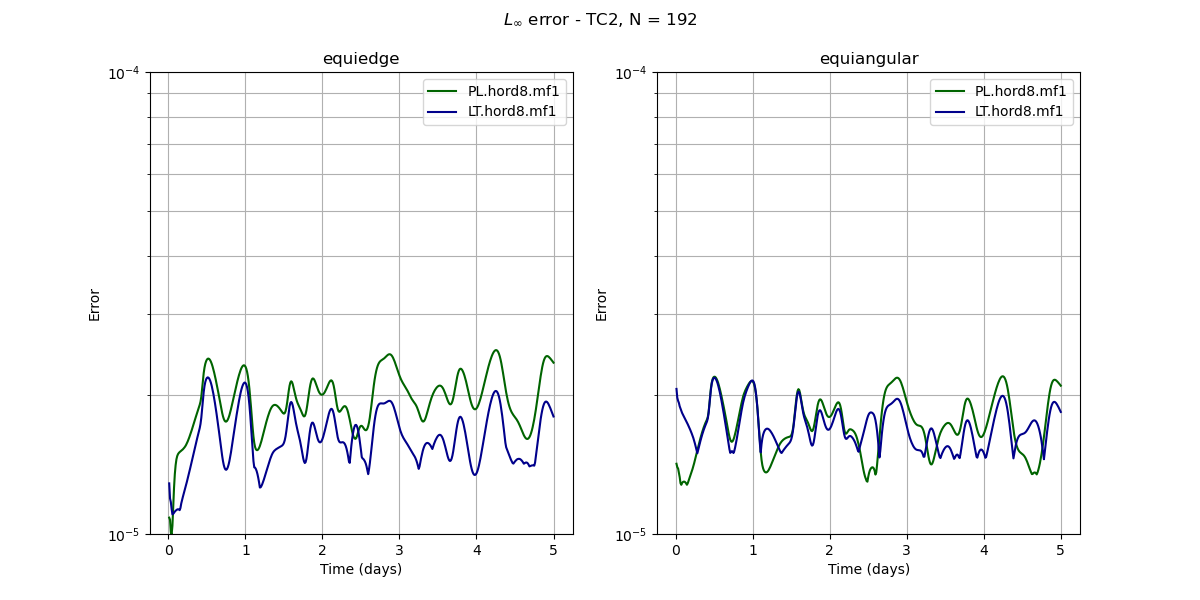
\includegraphics[width=0.8\linewidth]{tc2_C192_linf_errors}
	\caption{Geostrophic balanced flow test:
	$L_{\infty}$ relative error evolution for the fluid depth on the equi-edge grid (left)
		and on the equiangular grid (right) for 5 days and $N=192$.
		Blue lines indicate the use of the LT scheme, while green lines represent the PL scheme.
		All schemes use the monotonic PPM (MONO). 
		Light colors do not use divergence damping (dd), whereas dark color use divergence damping coefficient of 0.12.
		\label{chp-advcs-sec-exp-sw-evol-linf}}
\end{figure}
\begin{figure}[!htb]
	\centering
	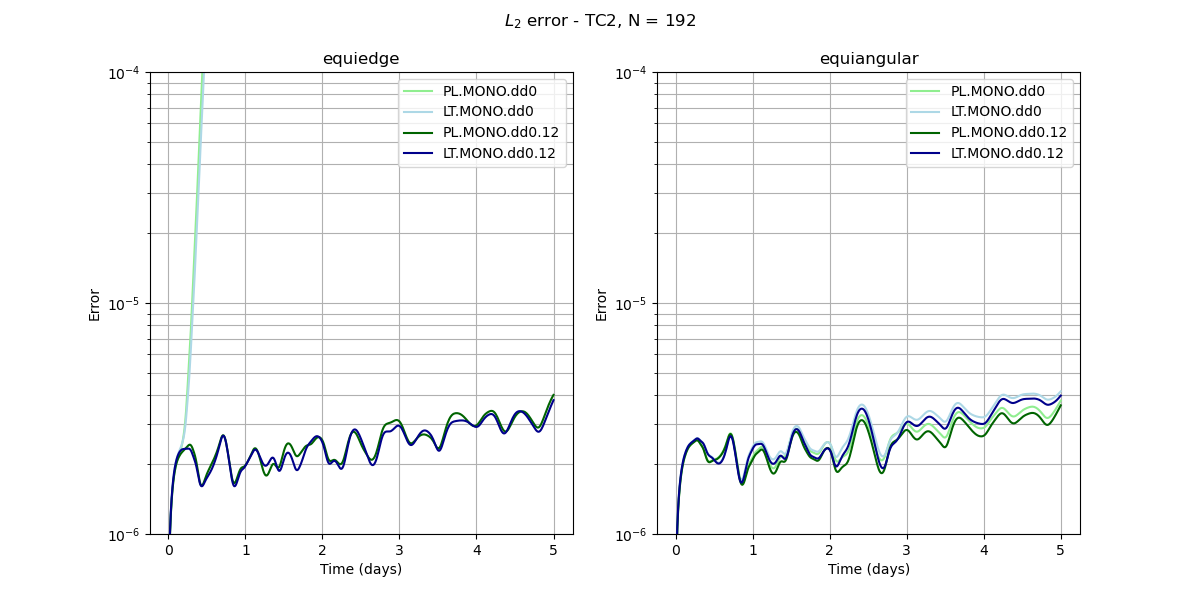
\includegraphics[width=0.8\linewidth]{tc2_C192_l2_errors}
	\caption{ As Figure \ref{chp-advcs-sec-exp-sw-evol-linf} but using the 
		$L_{2}$ norm.
		\label{chp-advcs-sec-exp-sw-evol-l2}}
\end{figure}

\newpage
In Figure \ref{chp-advcs-sec-exp-sw-evol-linf}, we present the evolution of the $L_{\infty}$ error in fluid depth over 5 days.
We can observe that for the equi-edge grid, before day 1, both schemes LT and PL become numerically unstable when no divergence damping is employed.
This behavior does not occur on the equiangular grid though.
Both schemes are numerically stable on both grids when divergence damping is included.
When the schemes are numerically stable, the errors of LT are only slightly smaller.
On the other hand, Figure \ref{chp-advcs-sec-exp-sw-evol-l2} shows that the $L_2$ error evolution of both schemes is similar for the equiangular grid, 
with PL being slightly smaller.
On the equi-edge grid, the $L_2$ error of LT is slightly smaller.

\begin{figure}[!h]
	\centering
	\begin{subfigure}{0.45\textwidth}
		\centering
		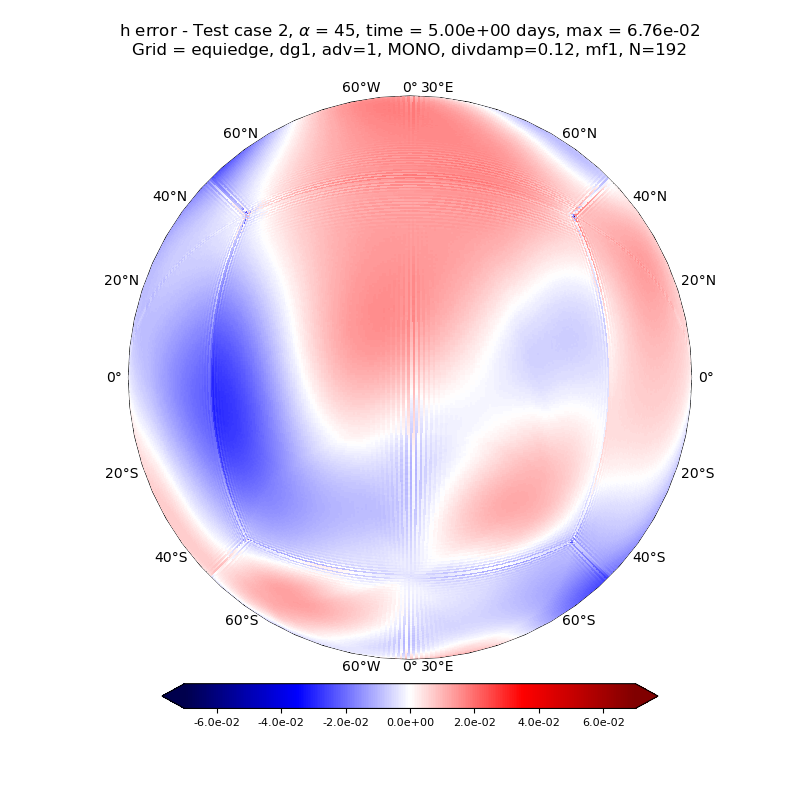
\includegraphics[width=1\linewidth]{h_error_tc2_t5_alpha45_C192_g0_dg1_adv1_hord8_dd0.12_mf1_tf5}
		\caption{PL scheme, max= $6.76\times10^{-2}$.\label{chp-advcs-sec-exp-sw1-errors-0a}}
	\end{subfigure}
	\begin{subfigure}{0.45\textwidth}
		\centering
		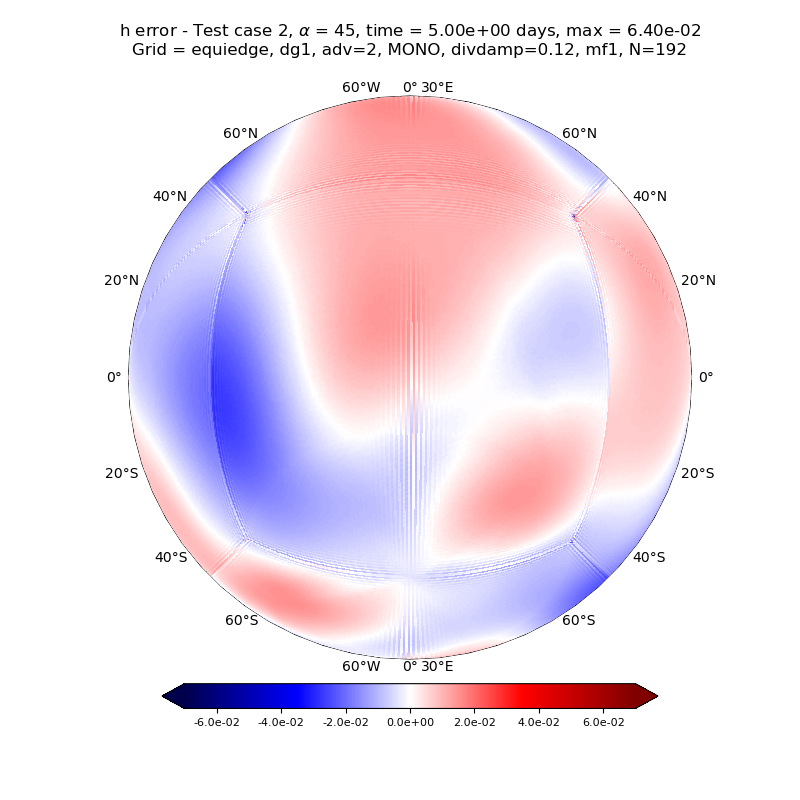
\includegraphics[width=1\linewidth]{h_error_tc2_t5_alpha45_C192_g0_dg1_adv2_hord8_dd0.12_mf1_tf5}
		\caption{LT scheme max= $6.40\times10^{-2}$.\label{chp-advcs-sec-exp-sw1-errors-0b}}
	\end{subfigure}
	\caption{
		Geostrophic balanced flow test: depth error distribution after 5 days using the monotonic PPM (MONO)
		with PL (left) and LT schemes (right) on the equi-edge grid (g0) with $N=192$. 
		These results uses a divergence damping coefficient equal to 0.12.
		\label{chp-advcs-sec-exp-sw1-errors-0}}
\end{figure}

\begin{figure}[!h]
	\centering
	\begin{subfigure}{0.45\textwidth}
		\centering
		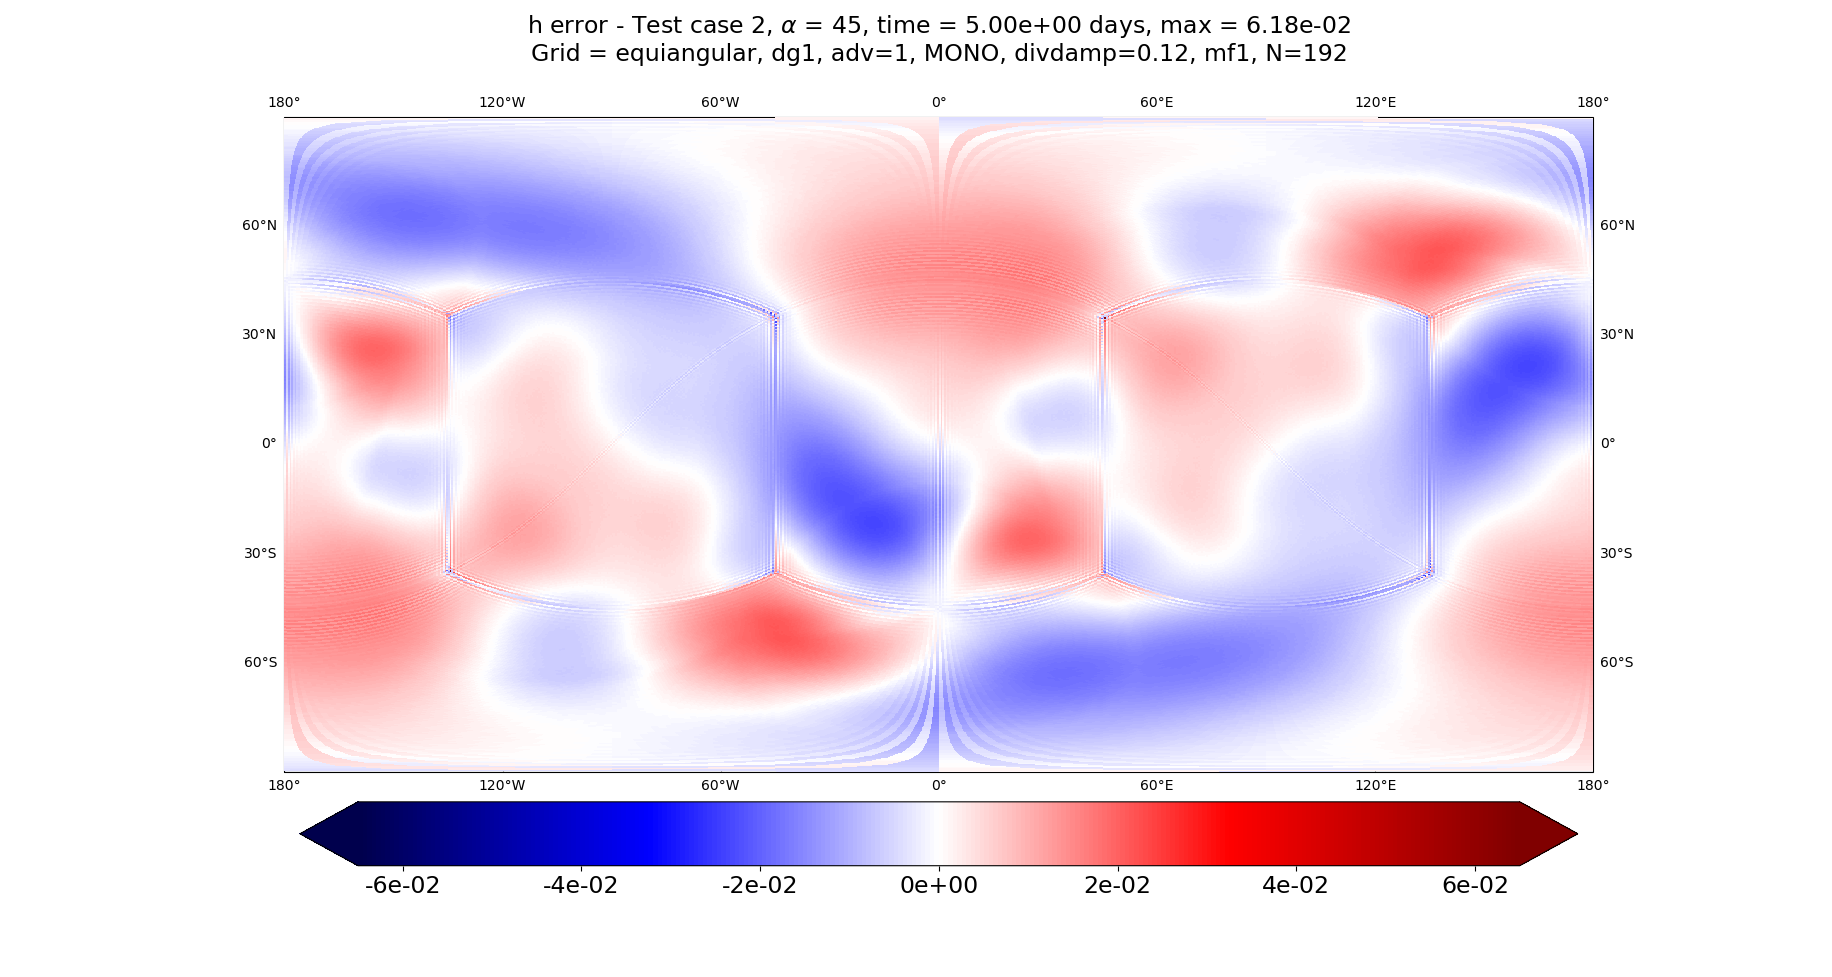
\includegraphics[width=1\linewidth]{h_error_tc2_t5_alpha45_C192_g2_dg1_adv1_hord8_dd0.12_mf1_tf5}
		\caption{PL scheme,  max= $6.18\times10^{-2}$.\label{chp-advcs-sec-exp-sw1-errors-2a}}
	\end{subfigure}
	\begin{subfigure}{0.45\textwidth}
		\centering
		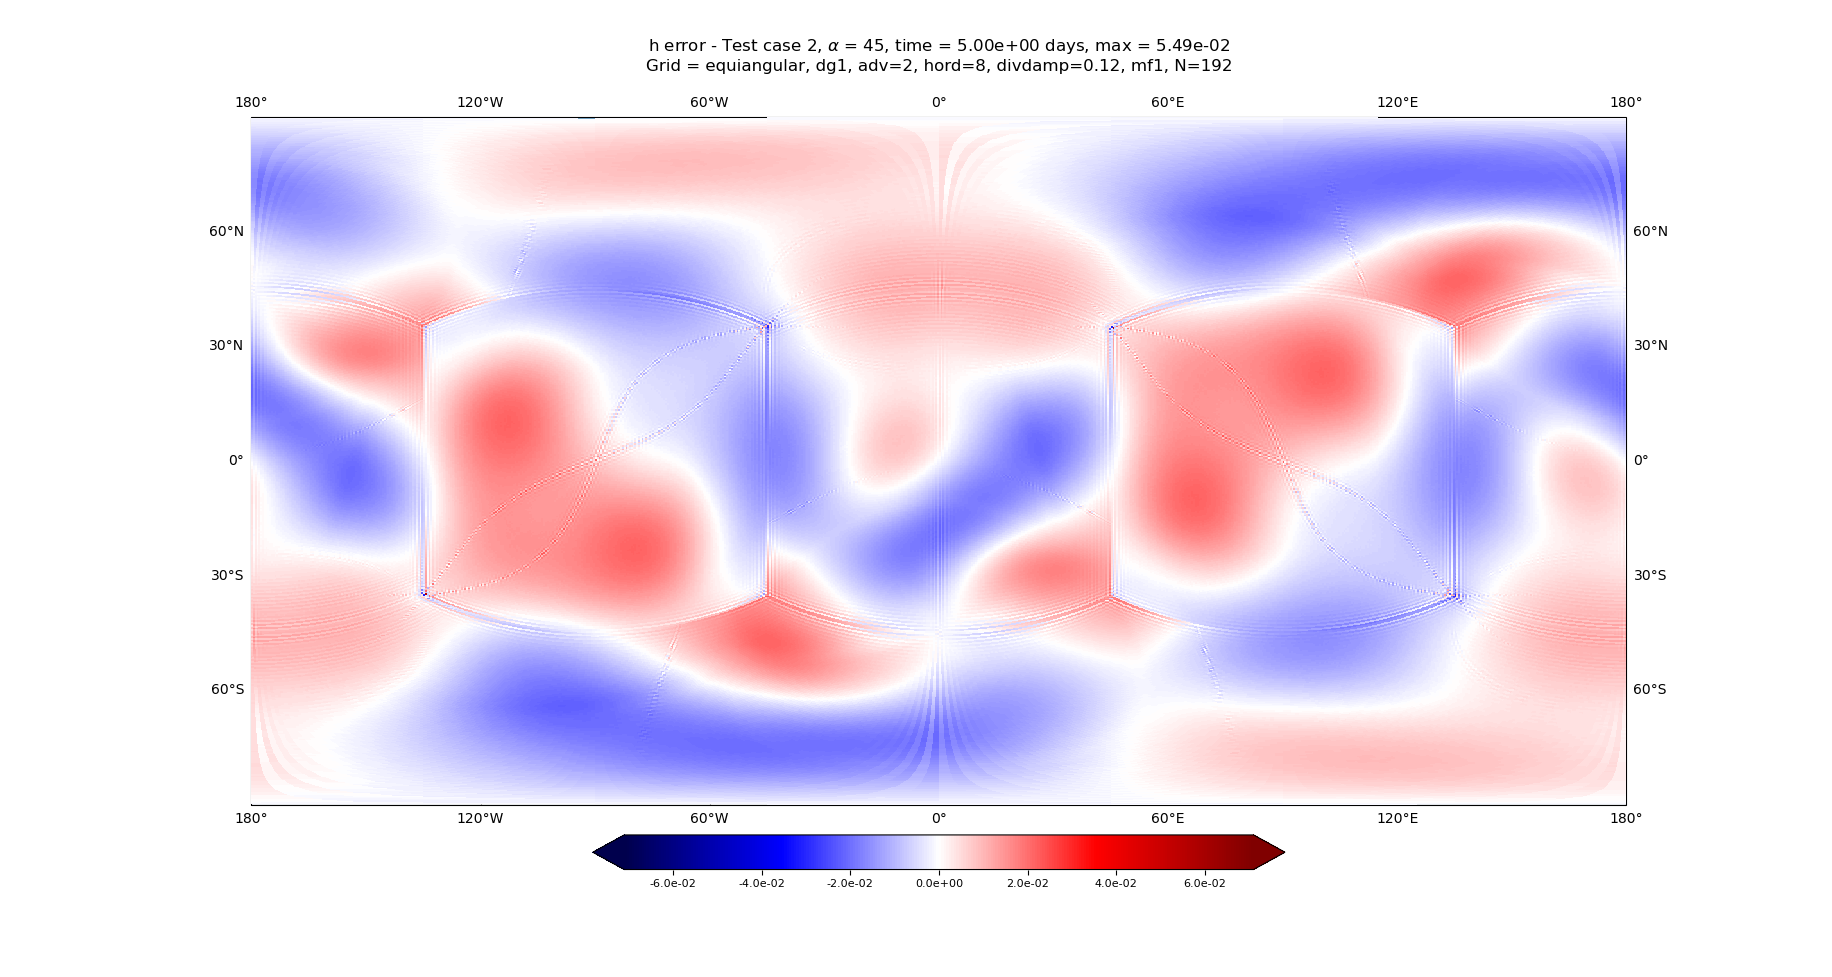
\includegraphics[width=1\linewidth]{h_error_tc2_t5_alpha45_C192_g2_dg1_adv2_hord8_dd0.12_mf1_tf5}
		\caption{LT scheme, max= $5.91\times10^{-2}$.\label{chp-advcs-sec-exp-sw1-errors-2b}}
	\end{subfigure}
	\caption{As Figure \ref{chp-advcs-sec-exp-sw1-errors-0} but using the equiangular grid (g2).
		\label{chp-advcs-sec-exp-sw1-errors-2}}
\end{figure}

\newpage

\begin{figure}[!h]
	\centering
	\begin{subfigure}{0.45\textwidth}
		\centering
		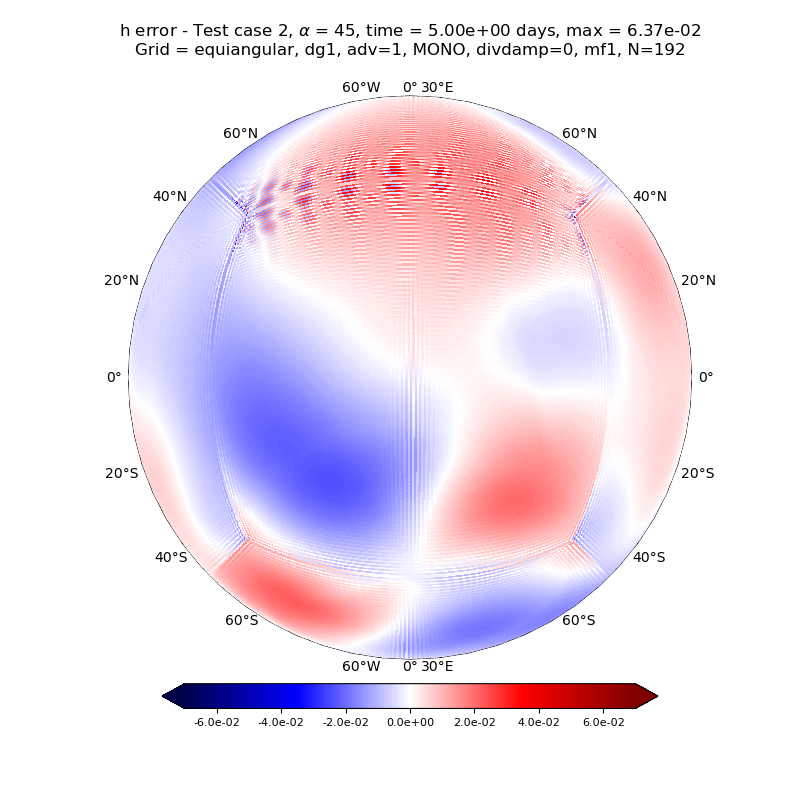
\includegraphics[width=1\linewidth]{h_error_tc2_t5_alpha45_C192_g2_dg1_adv1_hord8_dd0_mf1_tf5}
		\caption{PL scheme,  max= $6.37\times10^{-2}$.\label{chp-advcs-sec-exp-sw1-errors-3a}}
	\end{subfigure}
	\begin{subfigure}{0.45\textwidth}
		\centering
		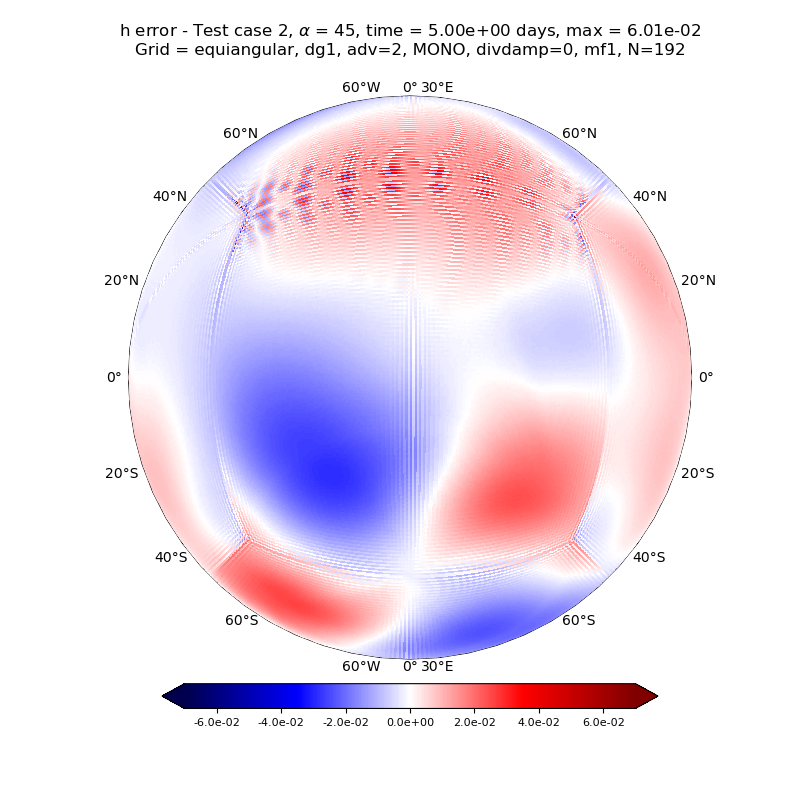
\includegraphics[width=1\linewidth]{h_error_tc2_t5_alpha45_C192_g2_dg1_adv2_hord8_dd0_mf1_tf5}
		\caption{LT scheme, max= $6.01\times10^{-2}$.\label{chp-advcs-sec-exp-sw1-errors-3b}}
	\end{subfigure}
	\caption{As Figure \ref{chp-advcs-sec-exp-sw1-errors-2} but using no divergence damping.\label{chp-advcs-sec-exp-sw1-errors-3}}
\end{figure}


In Figures \ref{chp-advcs-sec-exp-sw1-errors-0} and \ref{chp-advcs-sec-exp-sw1-errors-2} we show the final errors
for both grids with divergence damping.
The errors distribution is very similar for both schemes, and grid imprinting is still present, 
although the maximum errors, which occur at corners, are smaller for LT, indicating again that LT is slightly less sensitive to the corners.
In Figure \ref{chp-advcs-sec-exp-sw1-errors-2}, we show the errors of PL and LT on the equiangular grid without divergence damping.
Again, the errors of LT are slightly smaller. It is interesting to notice that in this case (no divergence damping), 
we can see some spurious waves being generated by the corners and affecting the solution at a cube edge, which does not occur when divergence damping is used.
At last, the errors without divergence damping on the equi-edge grid are not shown because the schemes are numerically unstable in that case.

\begin{figure}[!htb]
	\centering
	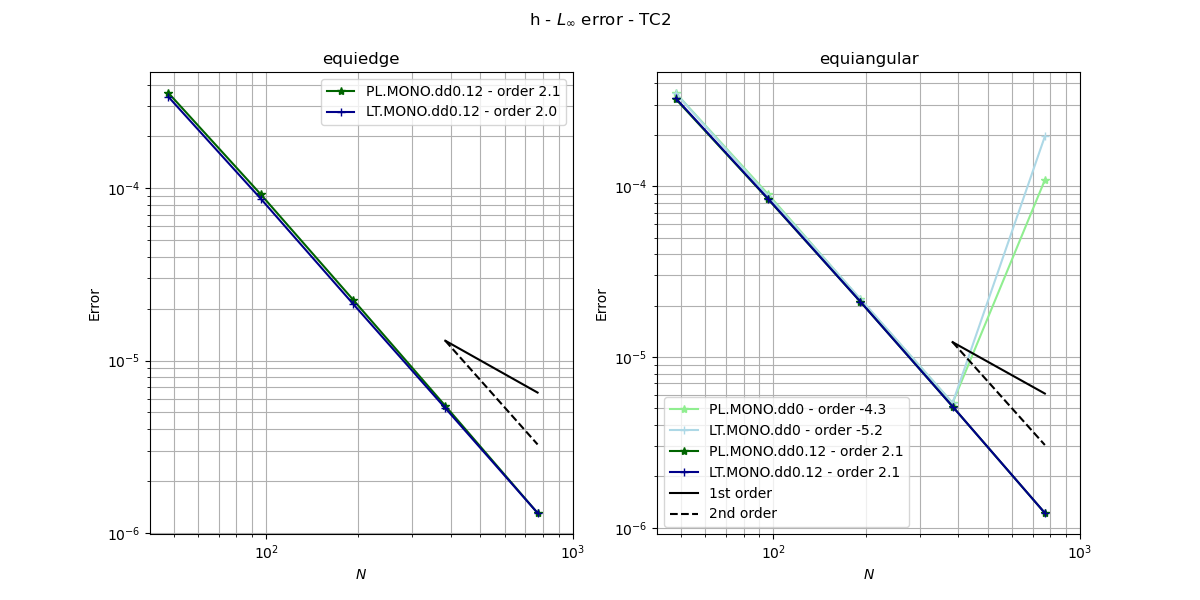
\includegraphics[width=0.9\linewidth]{h_linferror_tc2_alpha45}
	\caption{$L_{\infty}$ error of the fluid depth component for the geostrophic flow test case after 5 days
		for the equi-edge grid (left) and the equiangular grid (right)
		considering the schemes LT (dark and light blue lines) and the PL (dark and light green lines). 
		Light colors uses no divergence damping (dd) whereas dark colors use divergence damping.\label{chp-advcs-sec-exp-sw-linf}}
\end{figure}

\newpage
In Figure \ref{chp-advcs-sec-exp-sw-linf}, we show the convergence of the error in the $L_{\infty}$ for the fluid depth for all schemes and grids.
The results on the equi-edge grid without divergence damping are not shown because the scheme becomes numerically unstable in this case.
We can see that when using divergence damping, both the LT and PL schemes achieve second-order accuracy on both the equi-edge and equiangular grids.
However, we can that, when no divergence damping is employed, both schemes develop a very large error at a high resolution ($N=768$).
This result indicates that the equiangular grid may also develop numerical stability when there is divergence damping. 
However, this result shows that the equiangular grid is much more resilient to numerical instabilities than the equi-edge grid.

Finally, in Table \ref{sw-time}, we show the times needed by each scheme for different grids and values of $N$. 
It is clear that the LT scheme adds a very small cost, showing that this scheme does not degrade the computational performance of the shallow-water solver.

\begin{table}[!h]
	\begin{tabular}{|l|llll|}
		\hline
		\multicolumn{1}{|c|}{\multirow{2}{*}{\textbf{$N$}}} & \multicolumn{4}{c|}{Total runtime (seconds)}                                                                              \\ \cline{2-5} 
		\multicolumn{1}{|c|}{}                              & \multicolumn{1}{c|}{PL-g0}     & \multicolumn{1}{c|}{PL-g2}     & \multicolumn{1}{c|}{LT-g0}     & \multicolumn{1}{c|}{LT-g2} \\ \hline
		48                                                  & \multicolumn{1}{l|}{2.7762}    & \multicolumn{1}{l|}{2.9247}    & \multicolumn{1}{l|}{2.8379 }    & 2.8775                     \\ \hline
		96                                                  & \multicolumn{1}{l|}{12.2006}   & \multicolumn{1}{l|}{13.0276}   & \multicolumn{1}{l|}{12.5094}   & 13.1665                     \\ \hline
		192                                                 & \multicolumn{1}{l|}{89.2555}   & \multicolumn{1}{l|}{95.9484}   & \multicolumn{1}{l|}{90.1434}   & 96.4775                    \\ \hline
		384                                                 & \multicolumn{1}{l|}{719.8602}  & \multicolumn{1}{l|}{759.0486}  & \multicolumn{1}{l|}{705.6963}  & 743.4566                   \\ \hline
		768                                                 & \multicolumn{1}{l|}{7308.6683} & \multicolumn{1}{l|}{7529.9261} & \multicolumn{1}{l|}{7190.8789} & 7418.2488                  \\ \hline
	\end{tabular}
	\caption{Total runtime for the LT and PL schemes using the equi-edge grid (g0) and the equiangular grid (g2) for different values of $N$.
		The additional cost of the LT scheme is due to the computation of a second-order estimate of 1D departure points.}
\label{sw-time}
\end{table}


\newpage
\subsection{Flow over a mountain}
In this section, we present the flow over a mountain test case of \citet{will:1992}. 
This test uses the same initial condition as the geostrophic balance test case,
where $h$ follows Equation \eqref{duo-tc1} with $h_0=5960$ meters, and the winds follow Equation \eqref{duo-wind1}.
The rotation parameter $\alpha$ is set to 0, so the initial wind is purely zonal.
This test consider a bottom topography given by:
\begin{equation}
	b(\lambda,\phi) = 2000\bigg(1-\frac{r}{r_0}\bigg),
\end{equation}
where
\begin{equation}
    r =
	\begin{cases} 
		\sqrt{(\lambda-\lambda_0)^2 +  (\phi-\phi_0)^2}  & \text{if }  \sqrt{(\lambda-\lambda_0)^2 +  (\phi-\phi_0)^2} \leq r_0, \\
		r_0 &  \text{ otherwise,} \\
	\end{cases}
\end{equation}
$\lambda_0=-\frac{\pi}{4}$, $\phi_0=\frac{\pi}{6}$ and $r_0=\frac{\pi}{9}$. 
These parameters define the mountain over a cube corner (Figure \ref{sw-mountain-h-d0}).

\begin{figure}[!h]
	\centering
	\begin{subfigure}{0.48\textwidth}
		\centering
		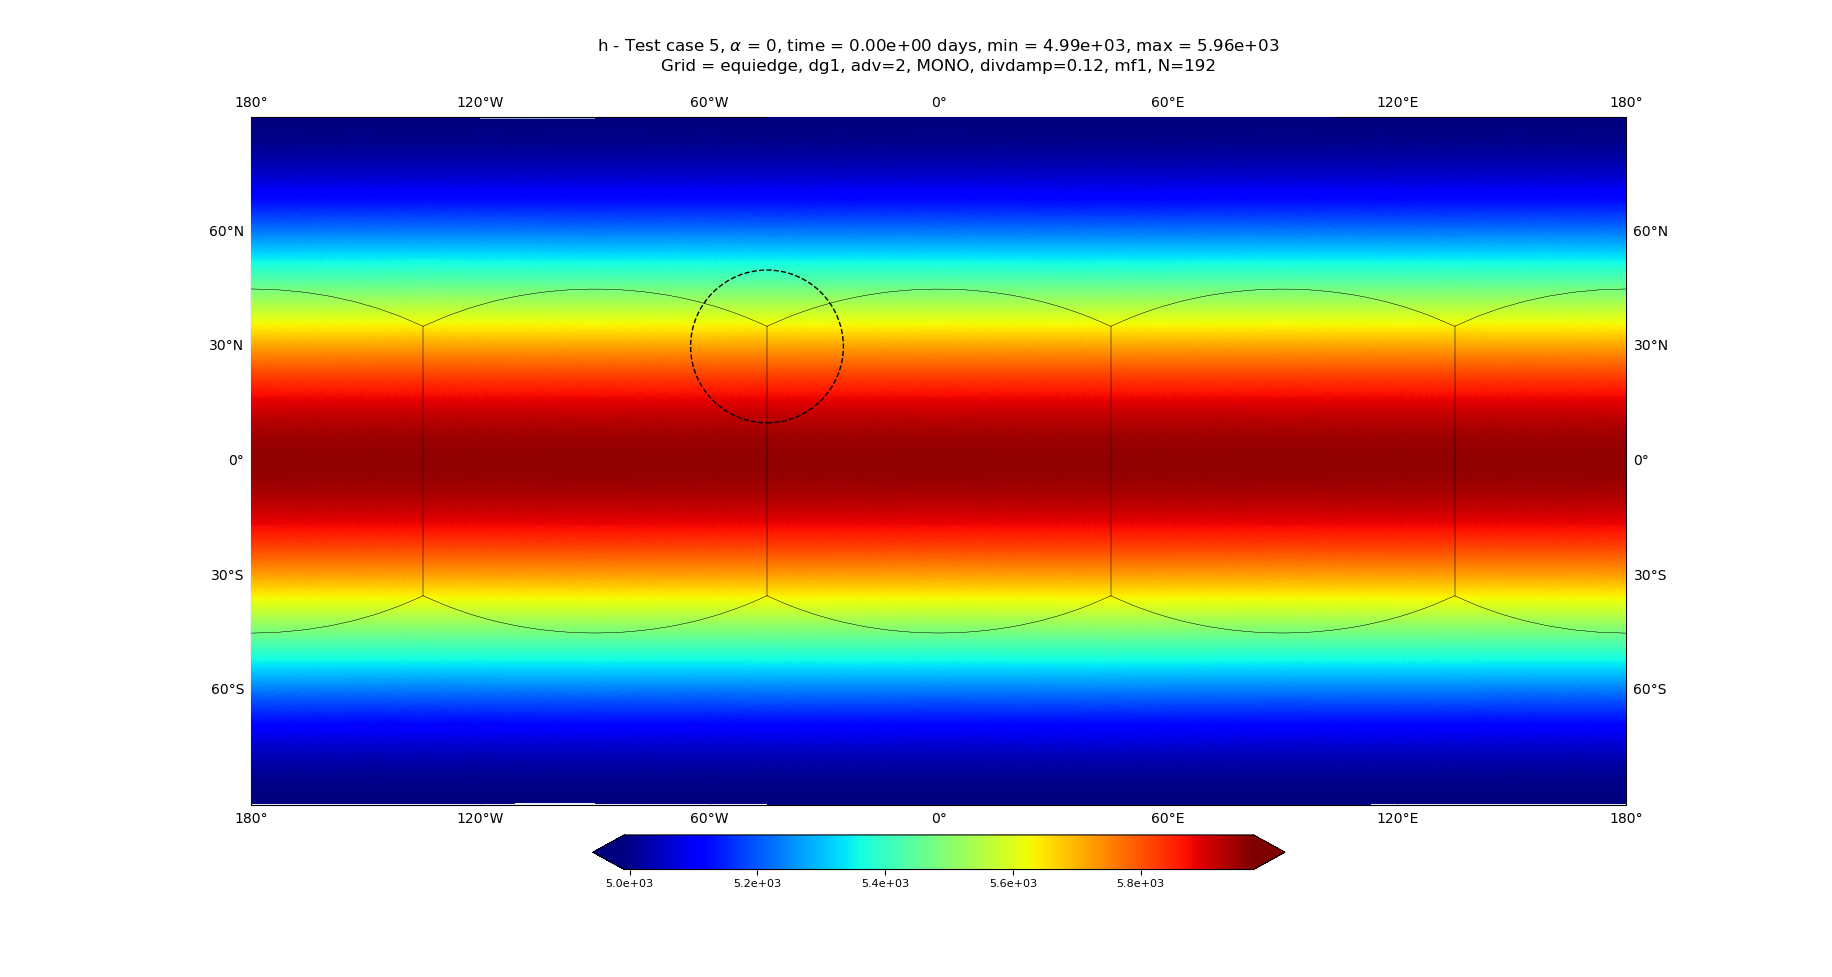
\includegraphics[width=1\linewidth]{h_tc5_t0_alpha0_C192_g0_dg1_adv2_hord8_dd0.12_mf1_tf15}
		\caption{Initial depth $h$.\label{sw-mountain-h-d0}}
	\end{subfigure}
	\begin{subfigure}{0.48\textwidth}
		\centering
		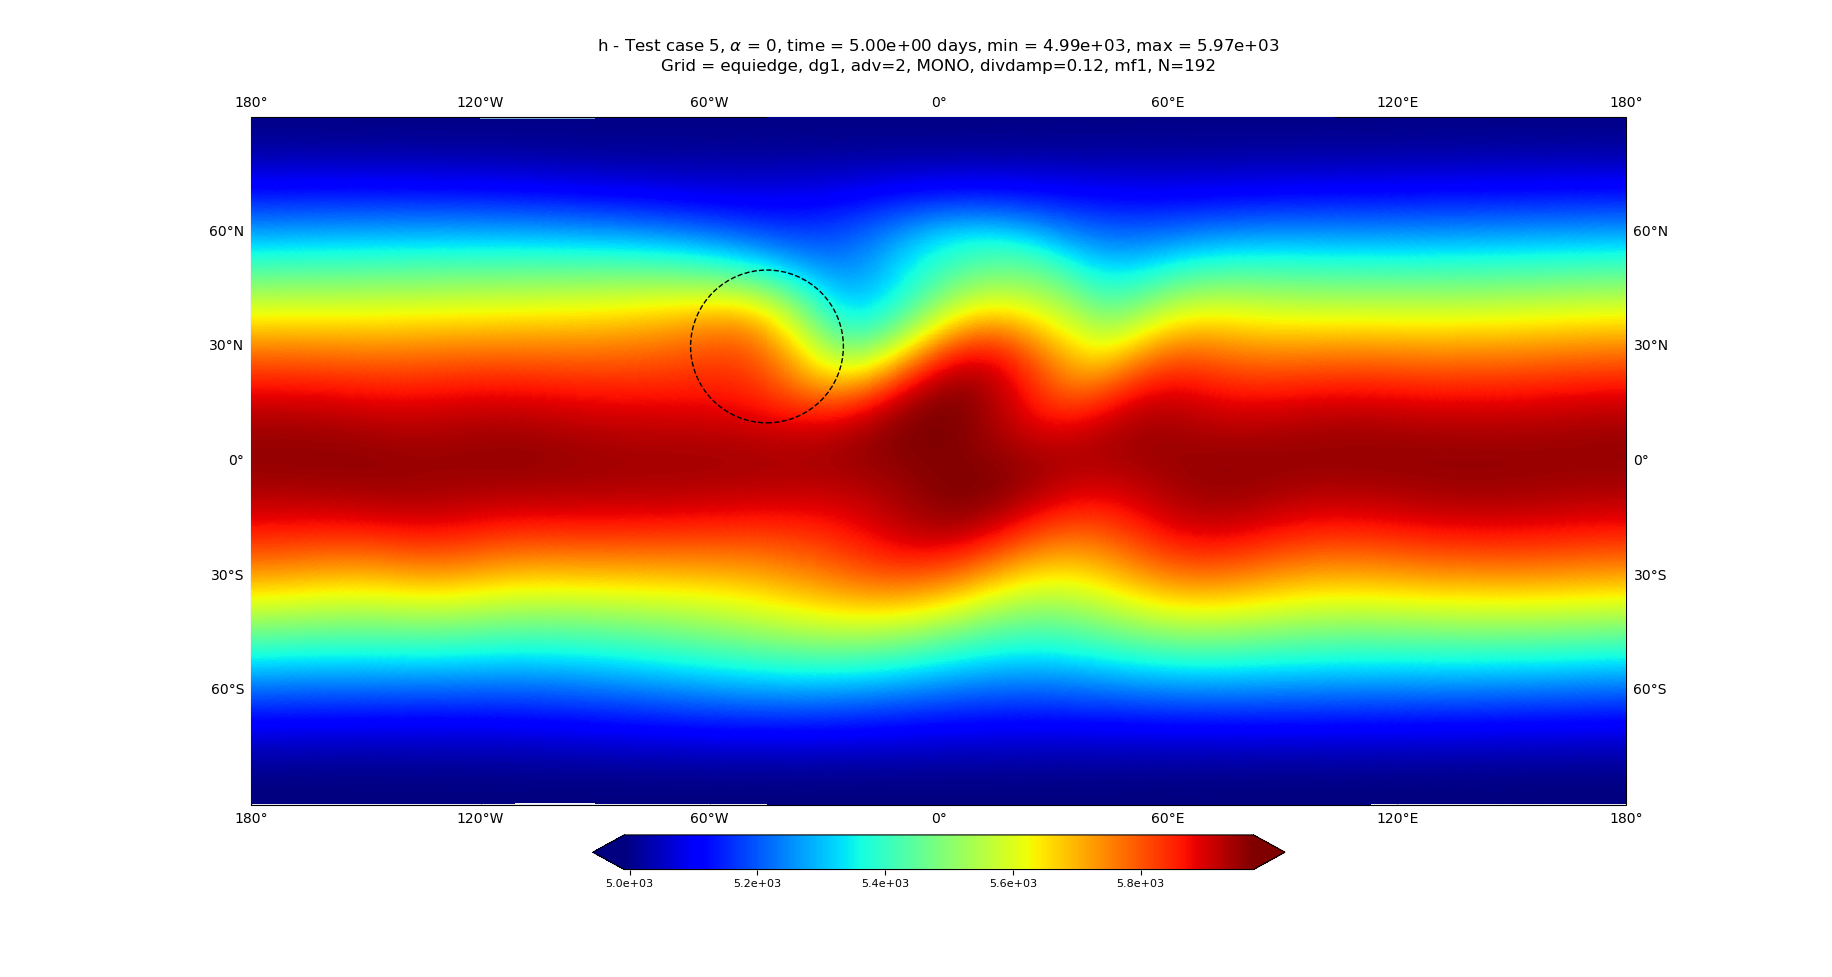
\includegraphics[width=1\linewidth]{h_tc5_t5_alpha0_C192_g0_dg1_adv2_hord8_dd0.12_mf1_tf15}
		\caption{Day 5.\label{sw-mountain-h-d5}}
	\end{subfigure}

	\begin{subfigure}{0.49\textwidth}
	\centering
	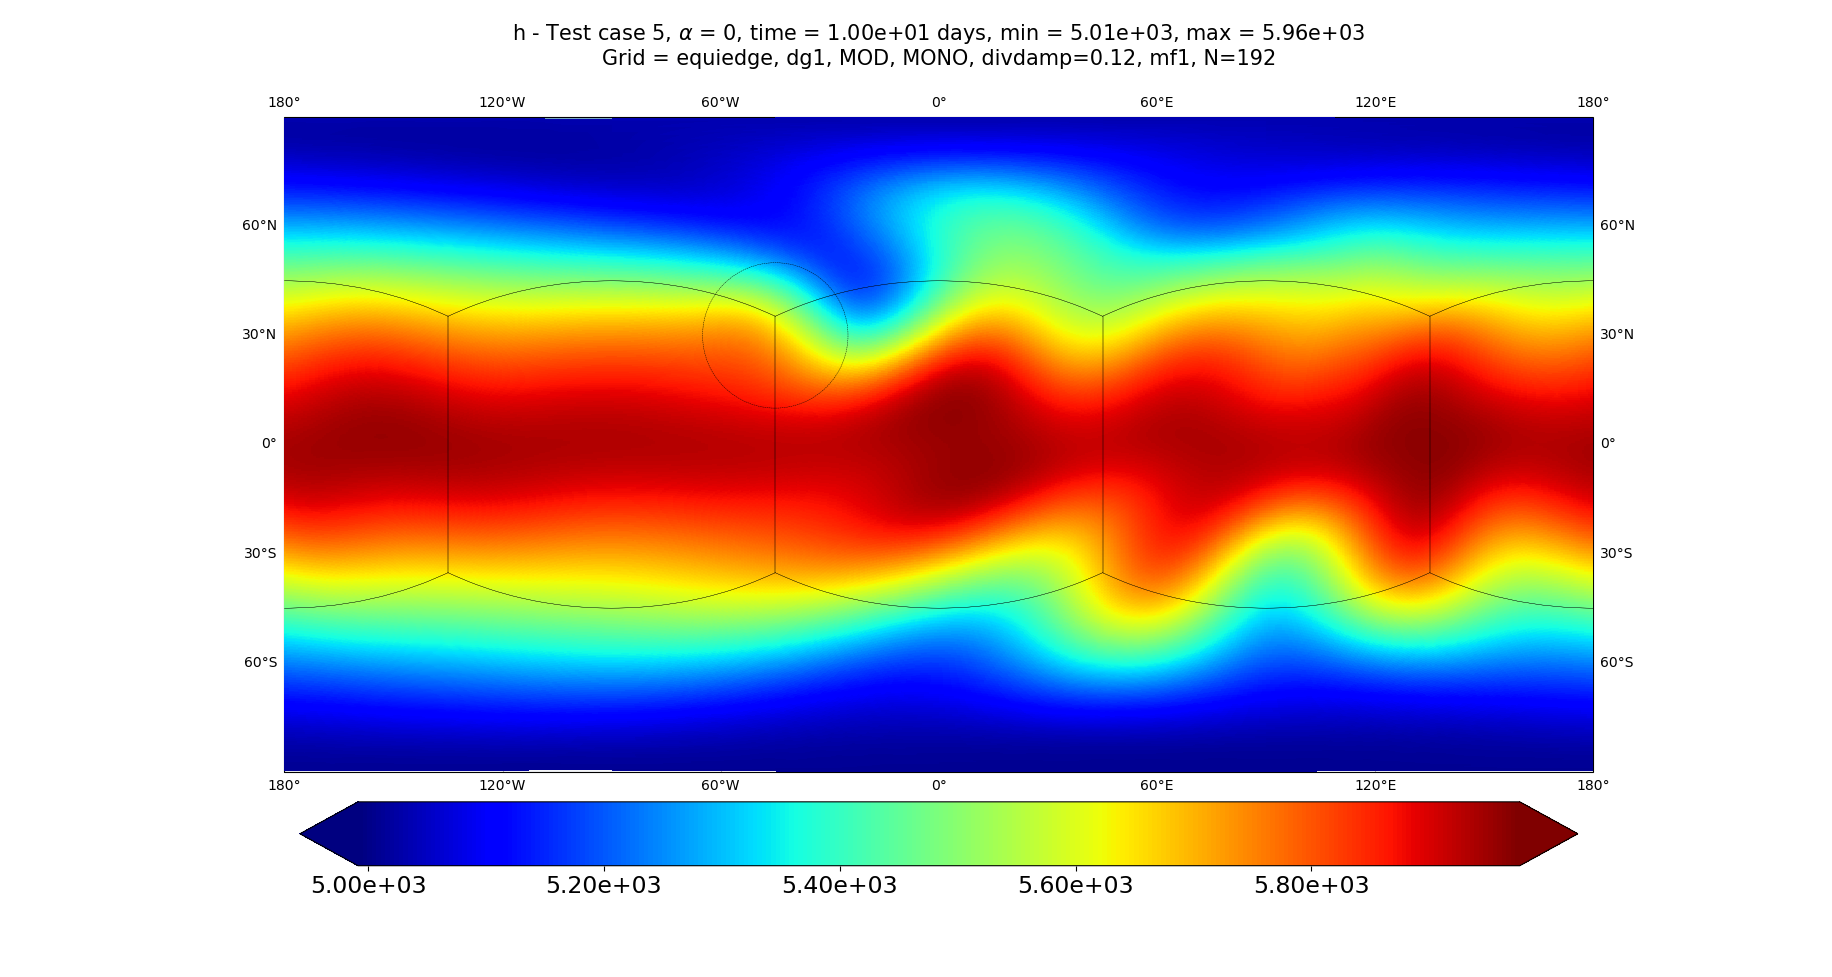
\includegraphics[width=1\linewidth]{h_tc5_t10_alpha0_C192_g0_dg1_adv2_hord8_dd0.12_mf1_tf15}
	\caption{Day 10.\label{sw-mountain-h-d10}}
\end{subfigure}
\begin{subfigure}{0.49\textwidth}
	\centering
	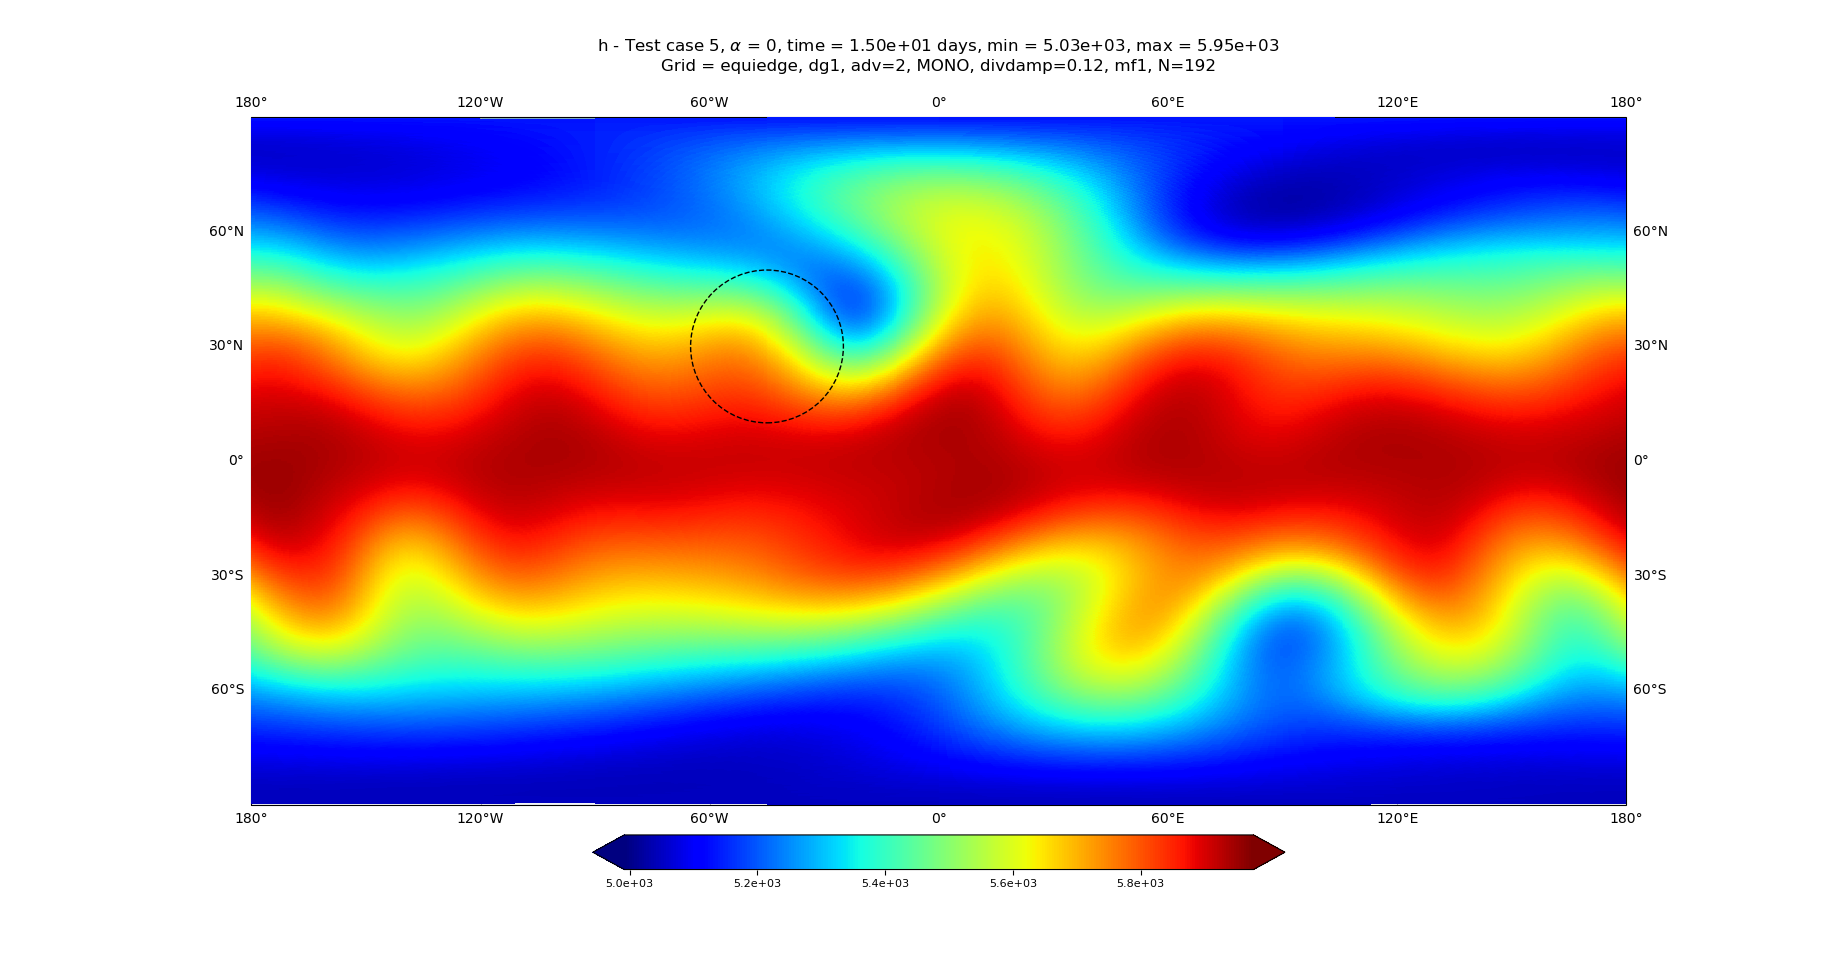
\includegraphics[width=1\linewidth]{h_tc5_t15_alpha0_C192_g0_dg1_adv2_hord8_dd0.12_mf1_tf15}
	\caption{Day 15.\label{sw-mountain-h-d15}}
\end{subfigure}
	\caption{Flow over a mountain: fluid depth initial condition (a) and after 5 (b), 10 (c), and 15 days (d). 
		We are using the LT scheme on the equi-edge grid with $N=192$ and a divergence damping coefficient equal to 0.12. The black circle shows the mountain's location.
		\label{sw-mountain-h}}
\end{figure}

We ran this test for 15 days.
In Figures \ref{sw-mountain-h}, we show the evolution of fluid depth over time,
specifically after 5, 10, and 15 days, using the LT scheme on an equi-edge grid with $N=192$ and divergence damping.
Figures \ref{sw-mountain-u} is similar but shows the meridional wind, illustrating the formation of a Rossby wave.
In Figure \ref{sw-mountain-div} we show the wind divergence at days 10 and 15.
It is clear from this last figure that we have a small amount of wind divergence, with a maximum absolute value equal to $6.7 \times 10^{-6}$, over to the mountain.
Hence, we expect that LT and PL should yield similar results.
\newpage

\begin{figure}[!h]
	\centering
	\begin{subfigure}{0.48\textwidth}
		\centering
		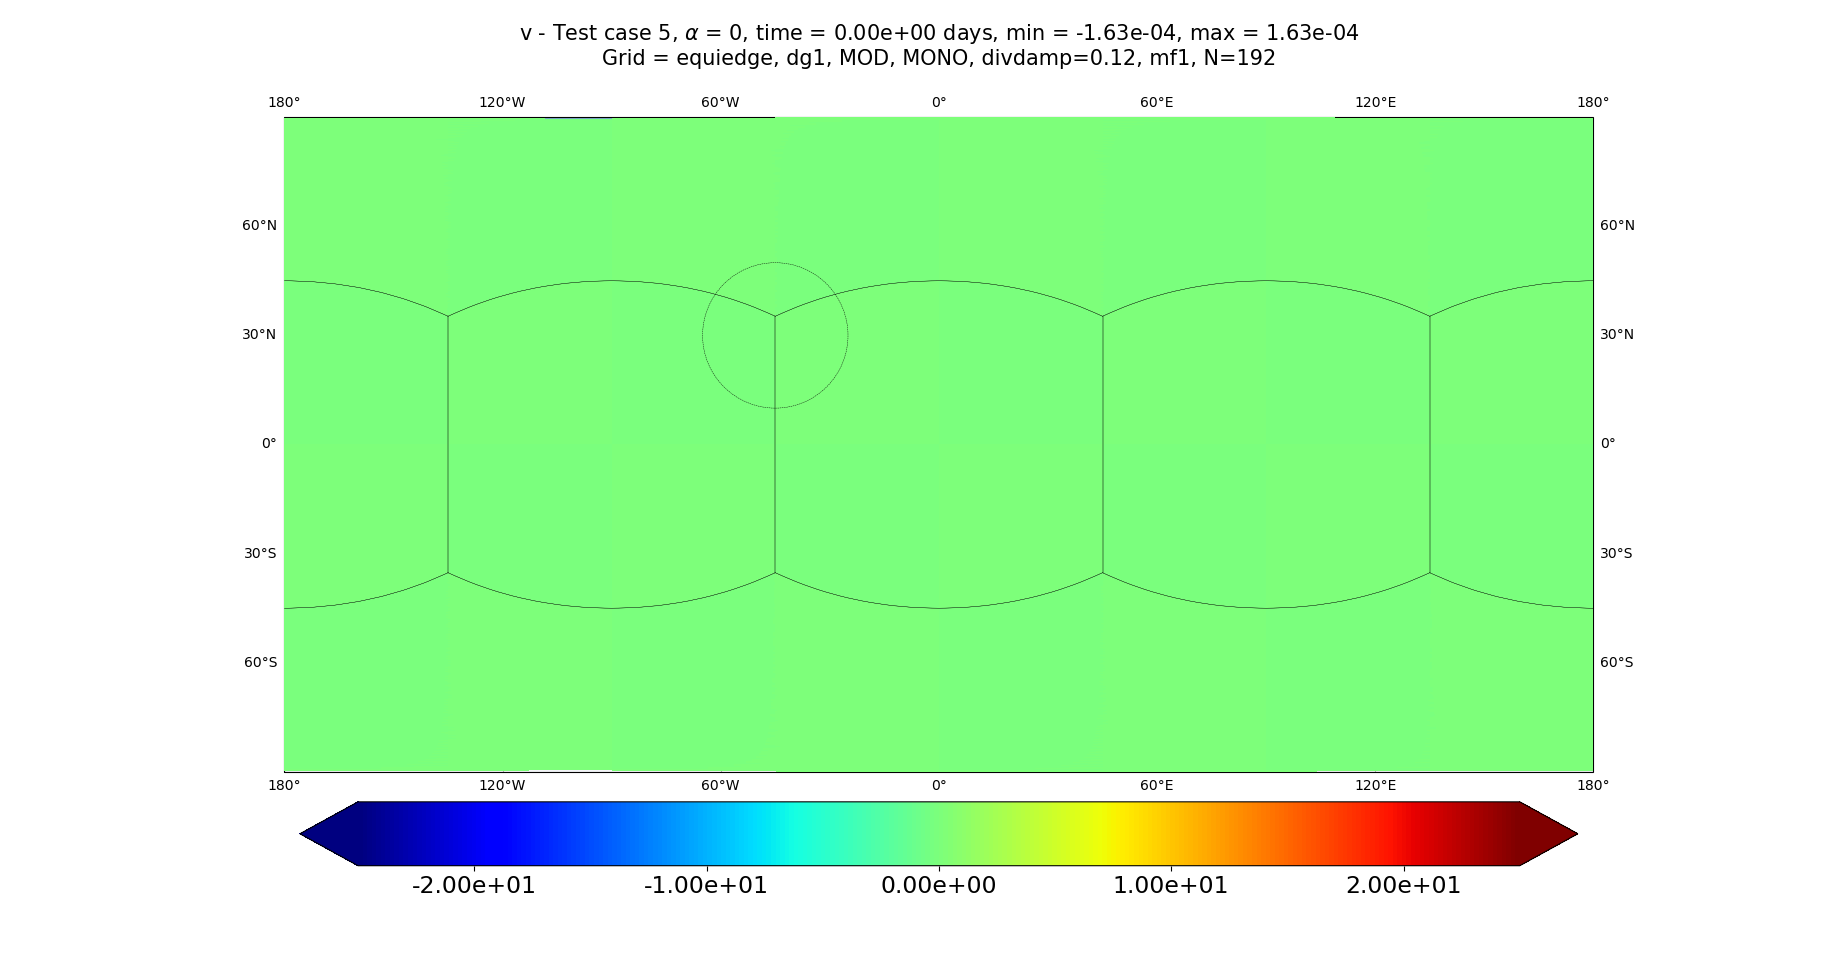
\includegraphics[width=1\linewidth]{v_tc5_t0_alpha0_C192_g0_dg1_adv2_hord8_dd0.12_mf1_tf15}
		\caption{Initial meridional wind $v_{\phi}$.\label{sw-mountain-v-d0}}
	\end{subfigure}
	\begin{subfigure}{0.48\textwidth}
		\centering
		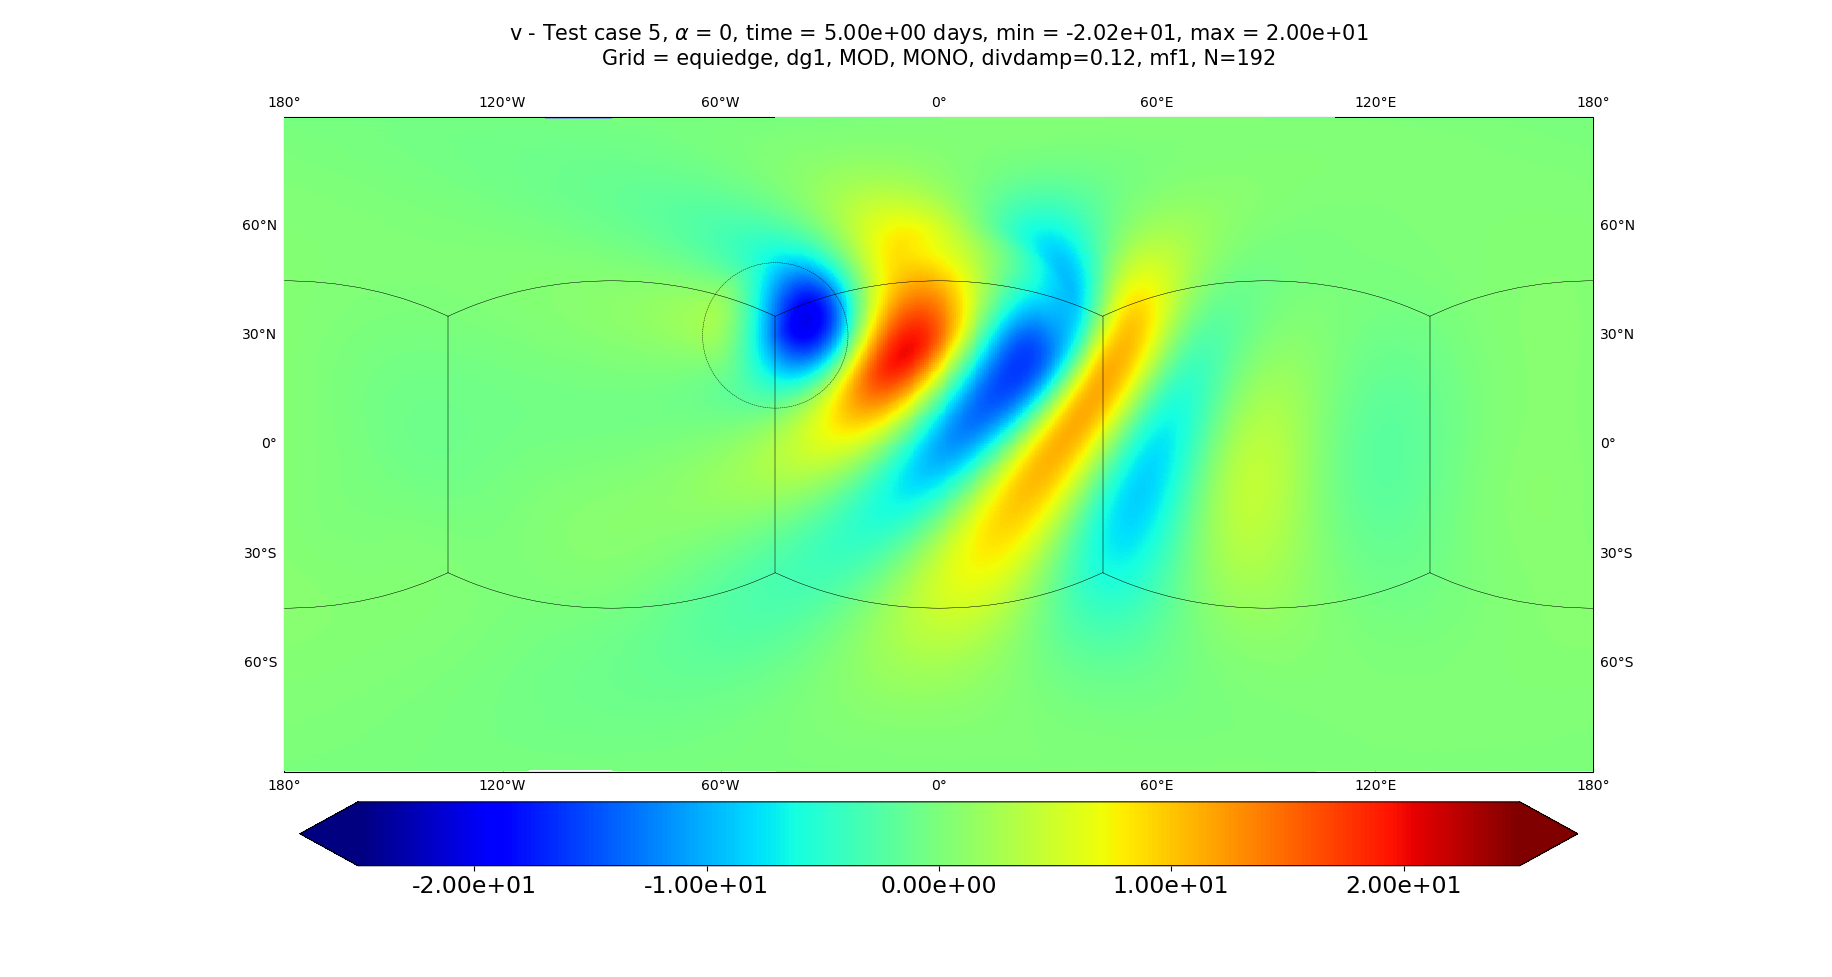
\includegraphics[width=1\linewidth]{v_tc5_t5_alpha0_C192_g0_dg1_adv2_hord8_dd0.12_mf1_tf15}
		\caption{Day 5.\label{sw-mountain-v-d5}}
	\end{subfigure}
	
	\begin{subfigure}{0.49\textwidth}
		\centering
		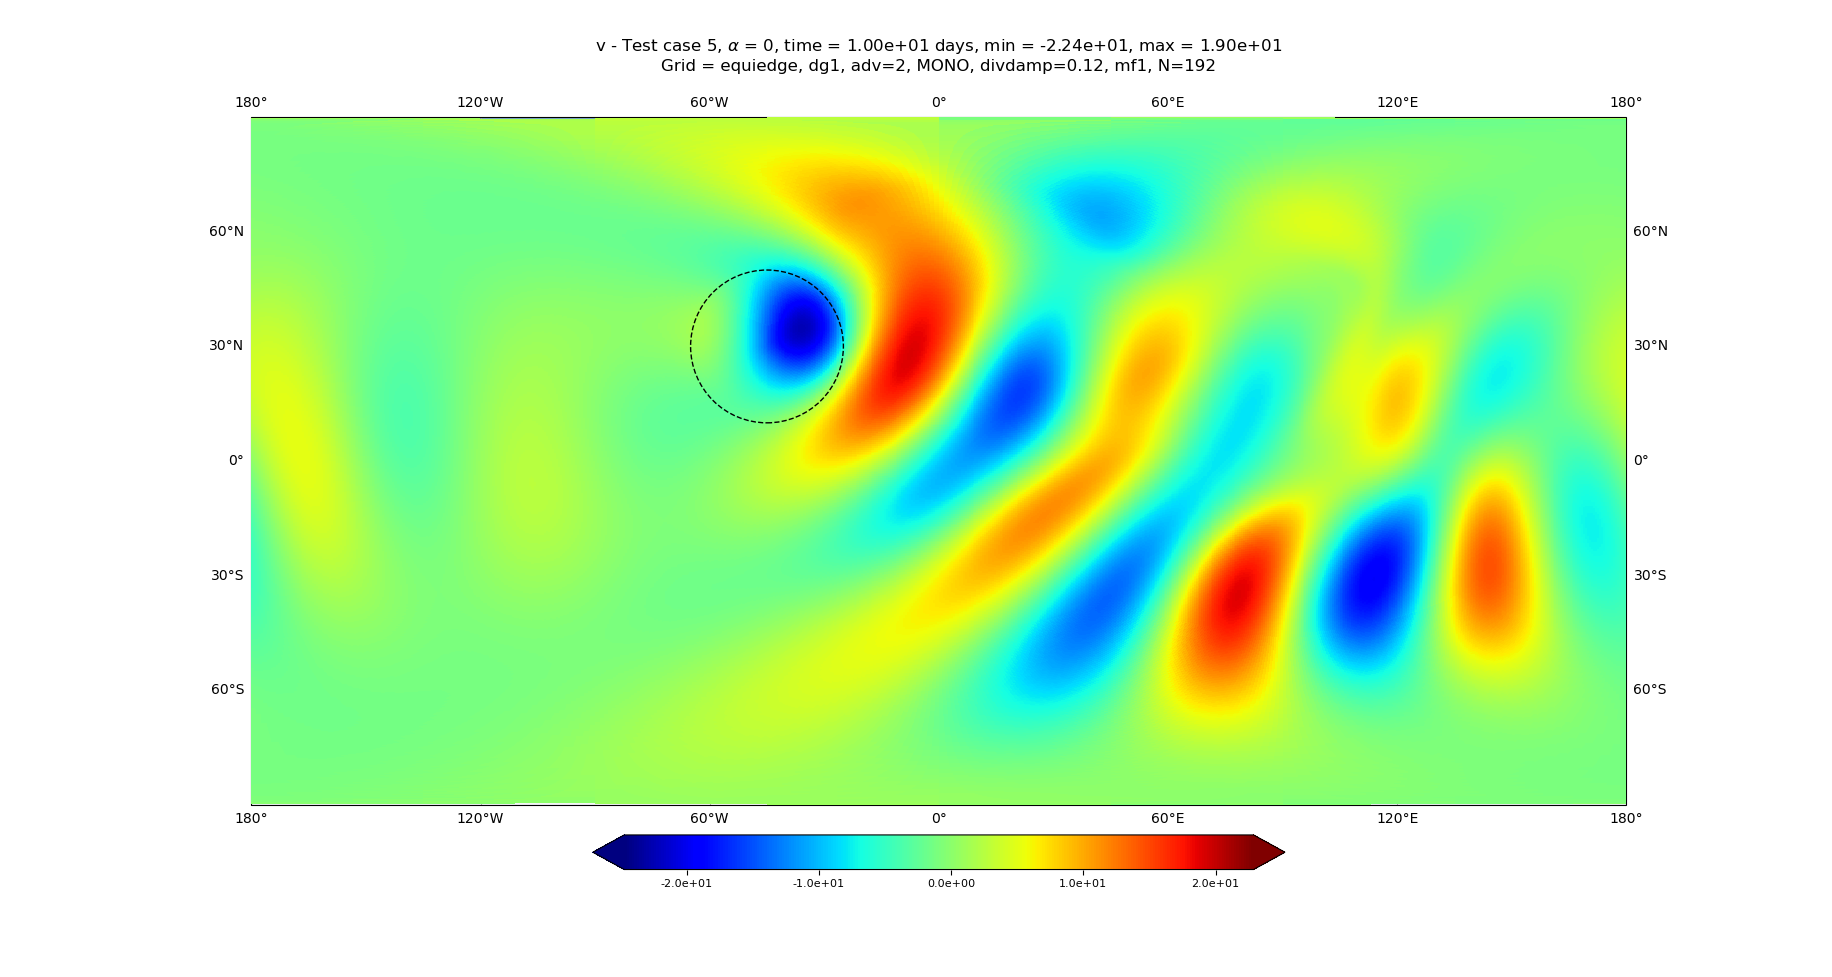
\includegraphics[width=1\linewidth]{v_tc5_t10_alpha0_C192_g0_dg1_adv2_hord8_dd0.12_mf1_tf15}
		\caption{Day 10.\label{sw-mountain-v-d10}}
	\end{subfigure}
	\begin{subfigure}{0.49\textwidth}
		\centering
		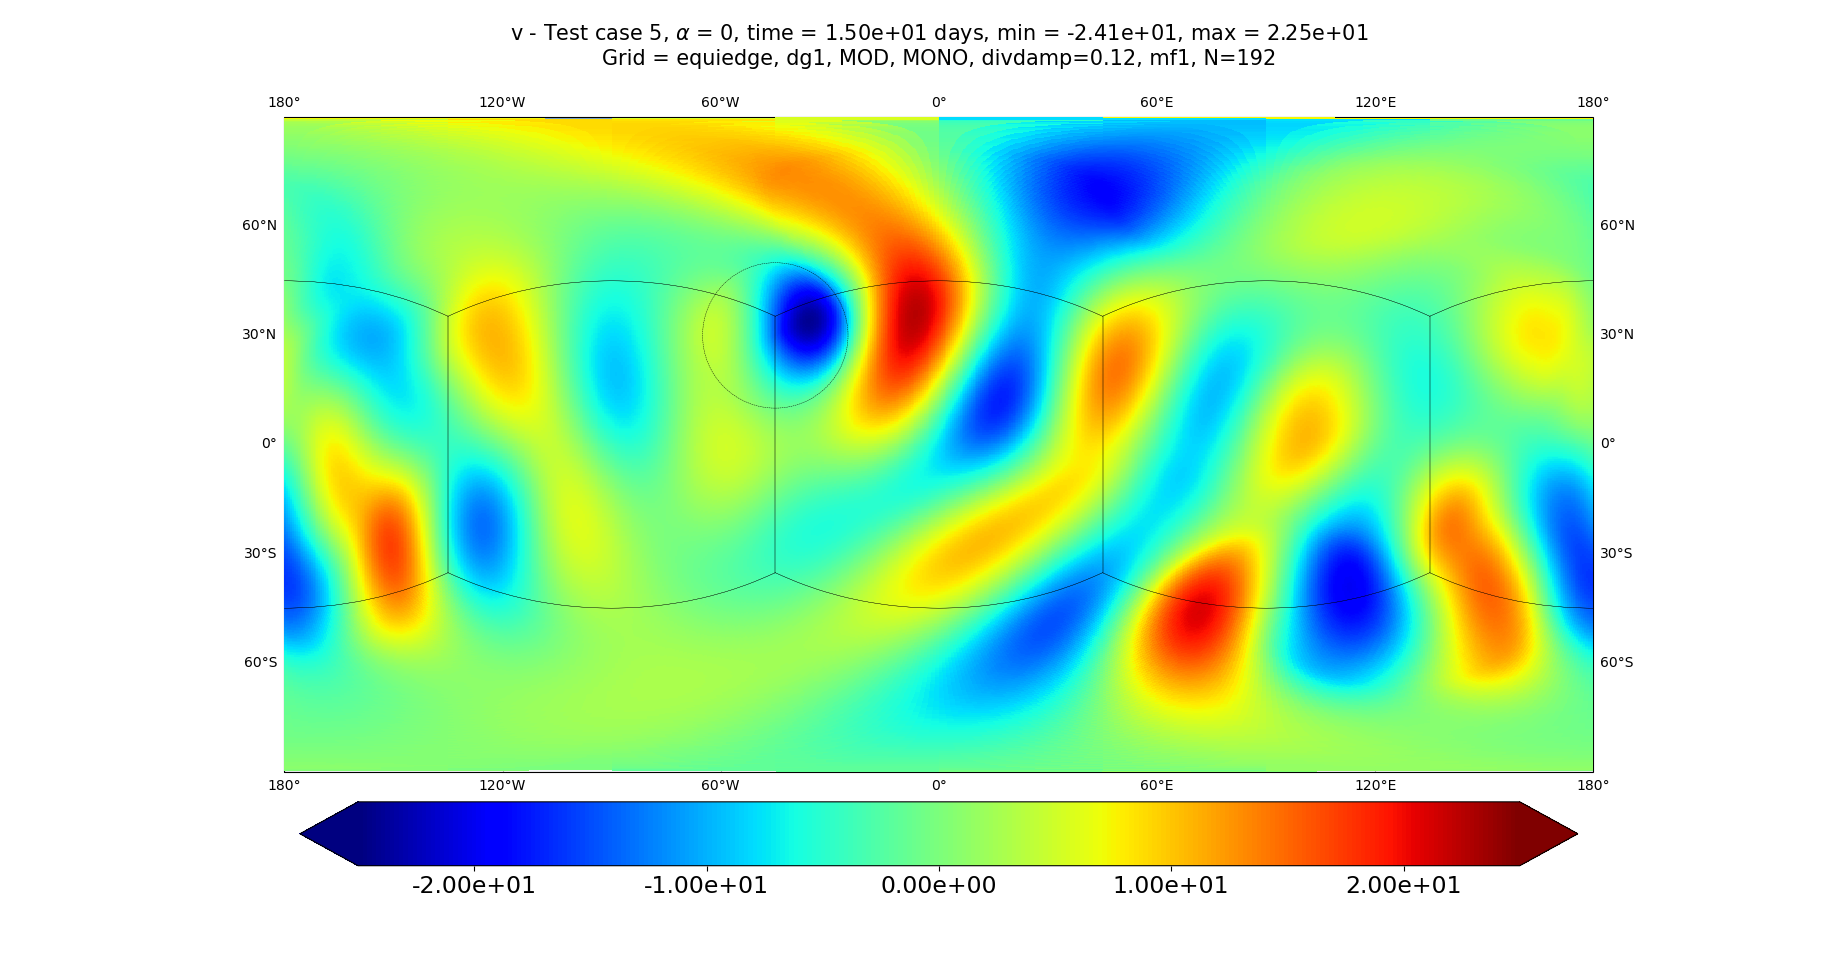
\includegraphics[width=1\linewidth]{v_tc5_t15_alpha0_C192_g0_dg1_adv2_hord8_dd0.12_mf1_tf15}
		\caption{Day 15.\label{sw-mountain-v-d15}}
	\end{subfigure}
	\caption{Flow over a mountain: meridional wind initial condition (a) and after 5 (b), 10 (c), and 15 days (d). 
		We are using the LT scheme on the equi-edge grid with $N=192$ and a divergence damping coefficient equal to 0.12. The black circle shows the mountain's location.
		\label{sw-mountain-u}}
\end{figure}
\begin{figure}[!h]
	\centering
	\begin{subfigure}{0.49\textwidth}
		\centering
		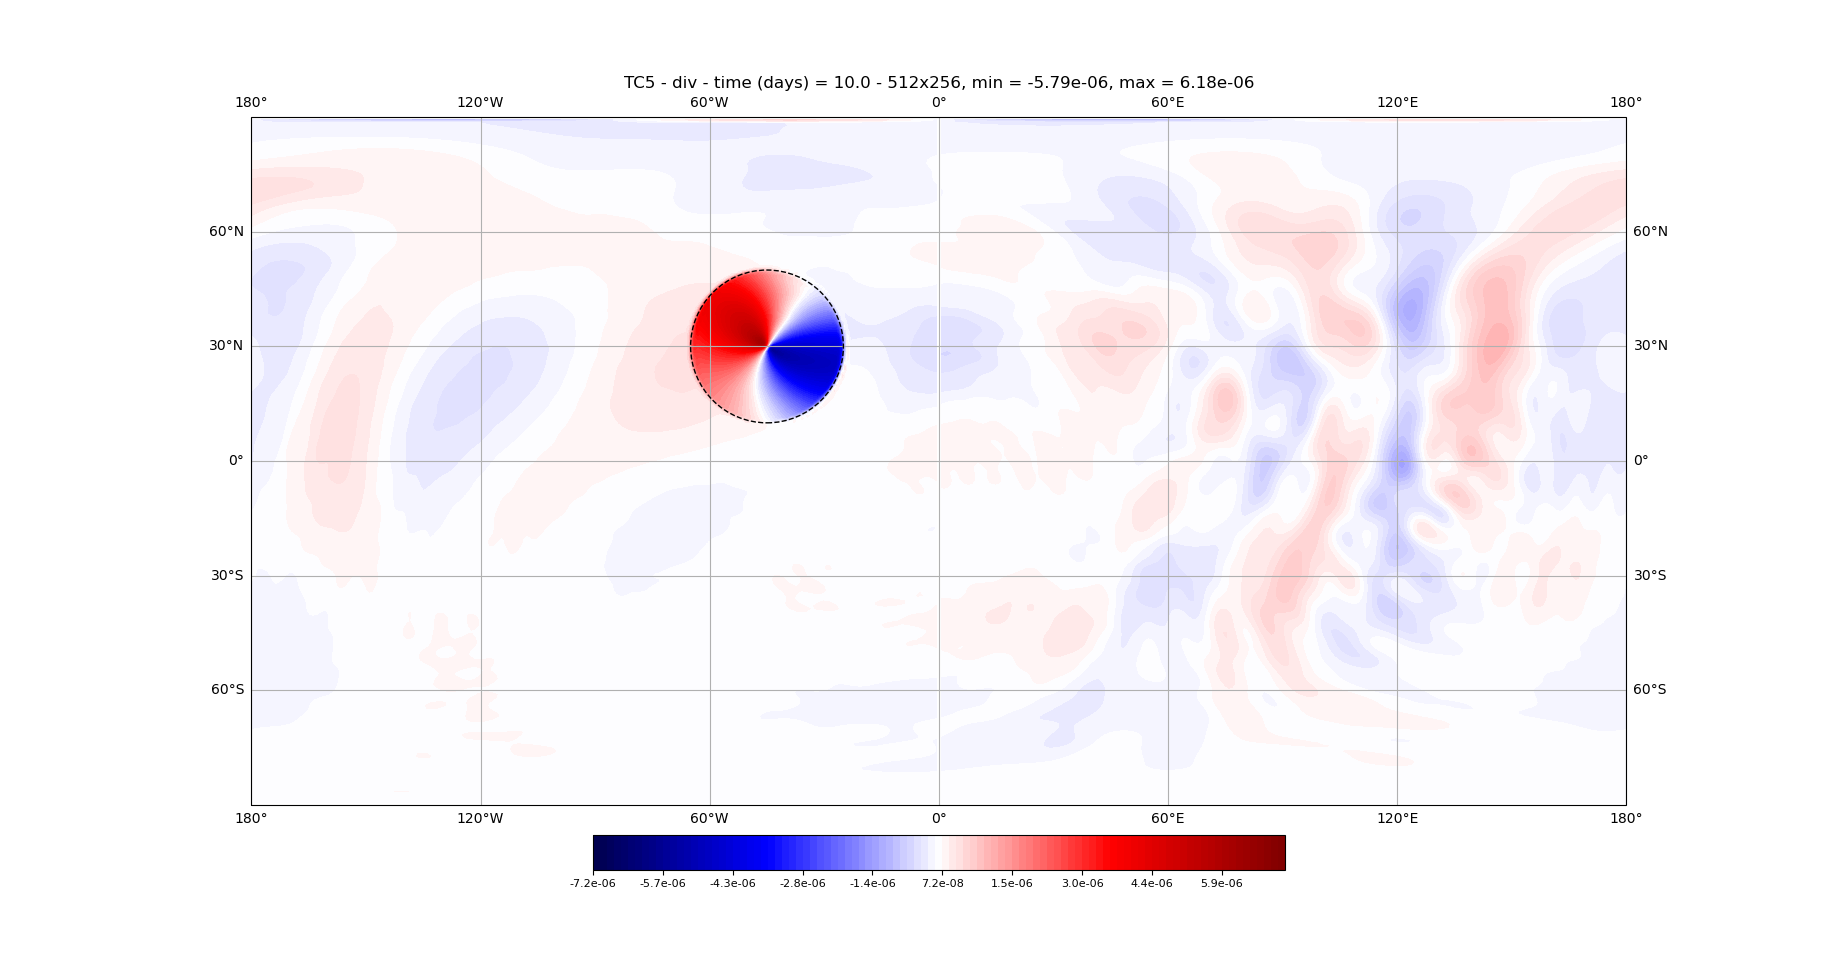
\includegraphics[width=1\linewidth]{eg_swe_run_ic5_cor1_div_t864000_512x256}
		\caption{Day 10.\label{sw-mountain-div-d10}}
	\end{subfigure}
	\begin{subfigure}{0.49\textwidth}
		\centering
		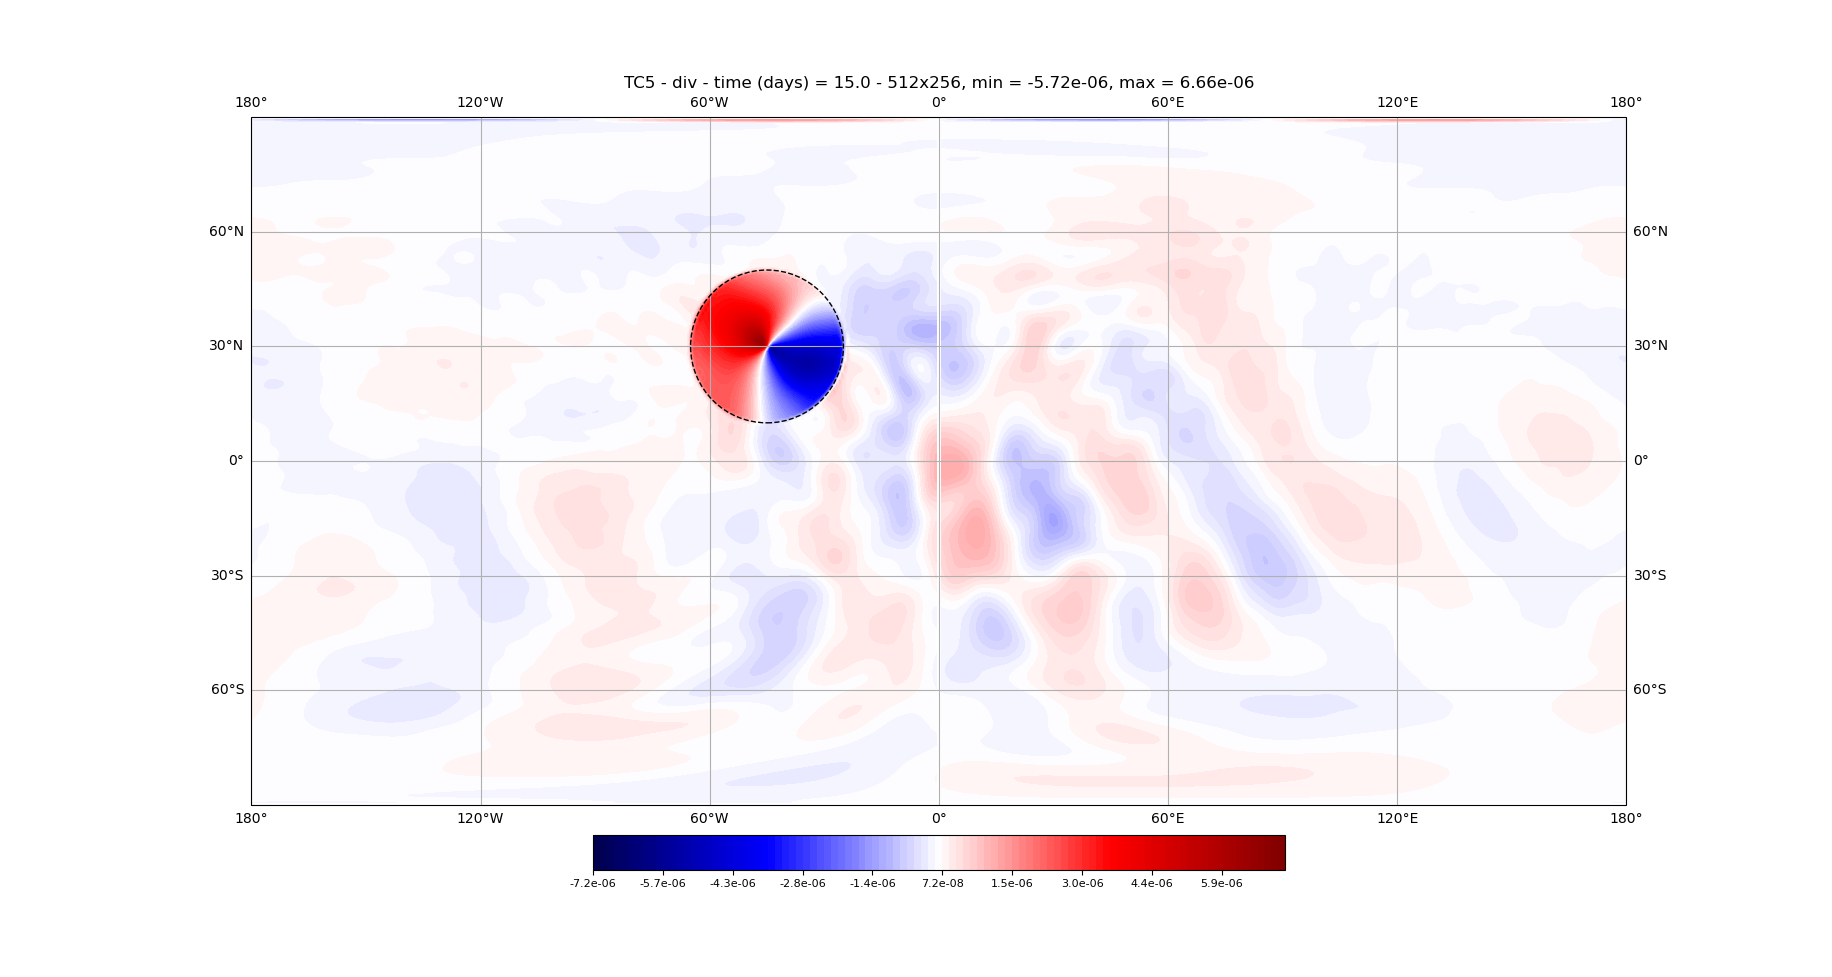
\includegraphics[width=1\linewidth]{eg_swe_run_ic5_cor1_div_t1296000_512x256}
		\caption{Day 15.\label{sw-mountain-div-d15}}
	\end{subfigure}
	\caption{Flow over a mountain: illustration of the wind divergence at days 10 and 5.
		The maximum absolute value of the divergence is $6.7\times 10^{-6}$.
		\label{sw-mountain-div}}
\end{figure}

To assess the accuracy of LT and PL schemes, we compute the errors using the ENDGame solution as a reference.
We are going to consider simulations with and without divergence damping on the equi-edge and equiangular grids with $N=192$.
We shall investigate the error evolution over time.
In fact, in Figures \ref{sw-mountain-h-error-linf} and \ref{sw-mountain-h-error-l2} we show the relative error evolution
for the fluid depth on the $L_{\infty}$ and $L_2$ norms.
It is clear that both PL and LT yield very similar results.
When divergence damping is employed, the errors do not grow very much. 
Otherwise, the errors may become much larger after day 12 at the equi-edge grid but not on the equiangular grid.
This simulation agrees with the previous simulation (geostrophic balance flow),
showing that the equiangular grid seems to be less susceptible to numerical instability.


\newpage
\begin{figure}[!htb]
	\centering
	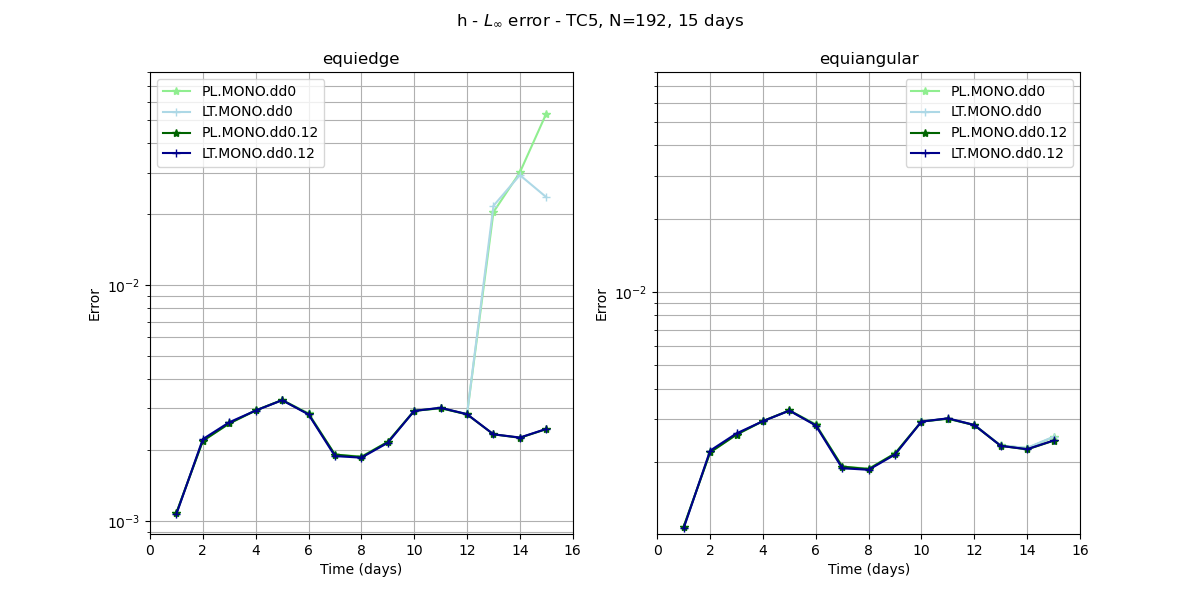
\includegraphics[width=0.9\linewidth]{h_linferror_tc5_N192}
	\caption{Flow over a mountain test case:
	$L_{\infty}$ relative error evolution for the fluid depth on the equi-edge grid (left)
and on the equiangular grid (right) for 5 days and $N=192$.
Blue lines indicate the use of the LT scheme, while green lines represent the PL scheme.
All schemes use the monotonic PPM (MONO). 
Light colors do not use divergence damping (dd), whereas dark color use divergence damping coefficient of 0.12.
The error is computed with a spacing of 1 day using ENDGame as the reference solution.
\label{sw-mountain-h-error-linf}}
\end{figure}

\begin{figure}[!htb]
	\centering
	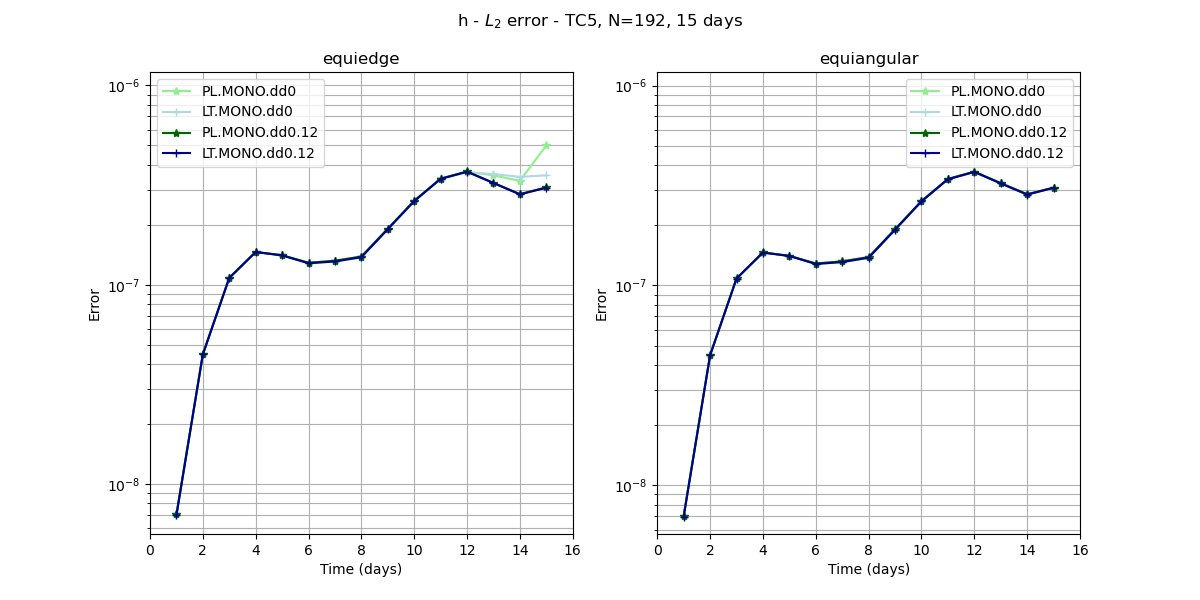
\includegraphics[width=0.9\linewidth]{h_l2error_tc5_N192}
	\caption{As Figure \ref{sw-mountain-h-error-linf} but using the $L_2$ norm.
		\label{sw-mountain-h-error-l2}}
\end{figure}

\newpage
\subsection{Rossby-Haurwitz wave}
The test considered in this section is the Rossby-Haurwitz wave case, as suggested by \citet{will:1992}.
The initial conditions are exact solutions to the barotropic vorticity equation.
Thus, the wind is divergence-free in this case.
The expressions of the initial fields may be found in \citet{will:1992}; we will omit them here.
The solutions should propagate the wave to east and maintain its shape.
Therefore, our goal in this test is to investigate the ability of the PL and LT schemes to preserve the wave shape.

\begin{figure}[!h]
	\centering
	\begin{subfigure}{0.48\textwidth}
		\centering
		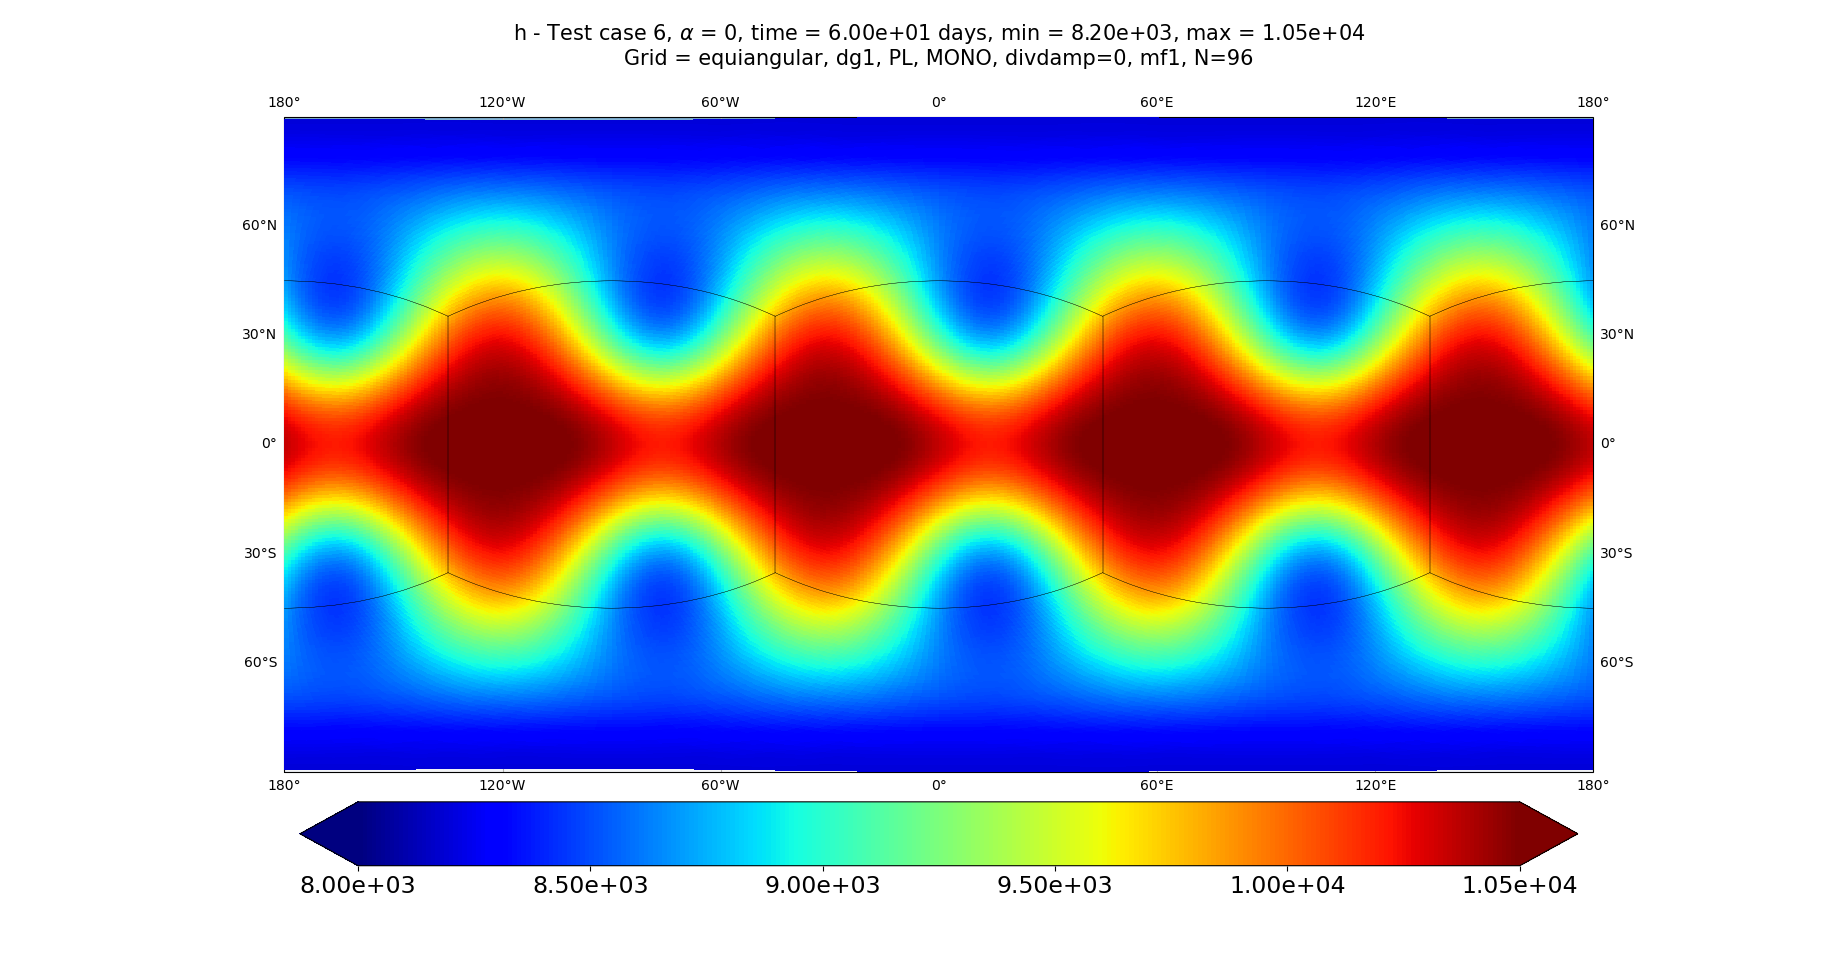
\includegraphics[width=1\linewidth]{h_tc6_t60_alpha0_C96_g2_dg1_adv1_hord8_dd0_mf1_tf105}
		\caption{PL at day 60.\label{sw-rossby-h-d60-pl}}
	\end{subfigure}
	\begin{subfigure}{0.48\textwidth}
		\centering
		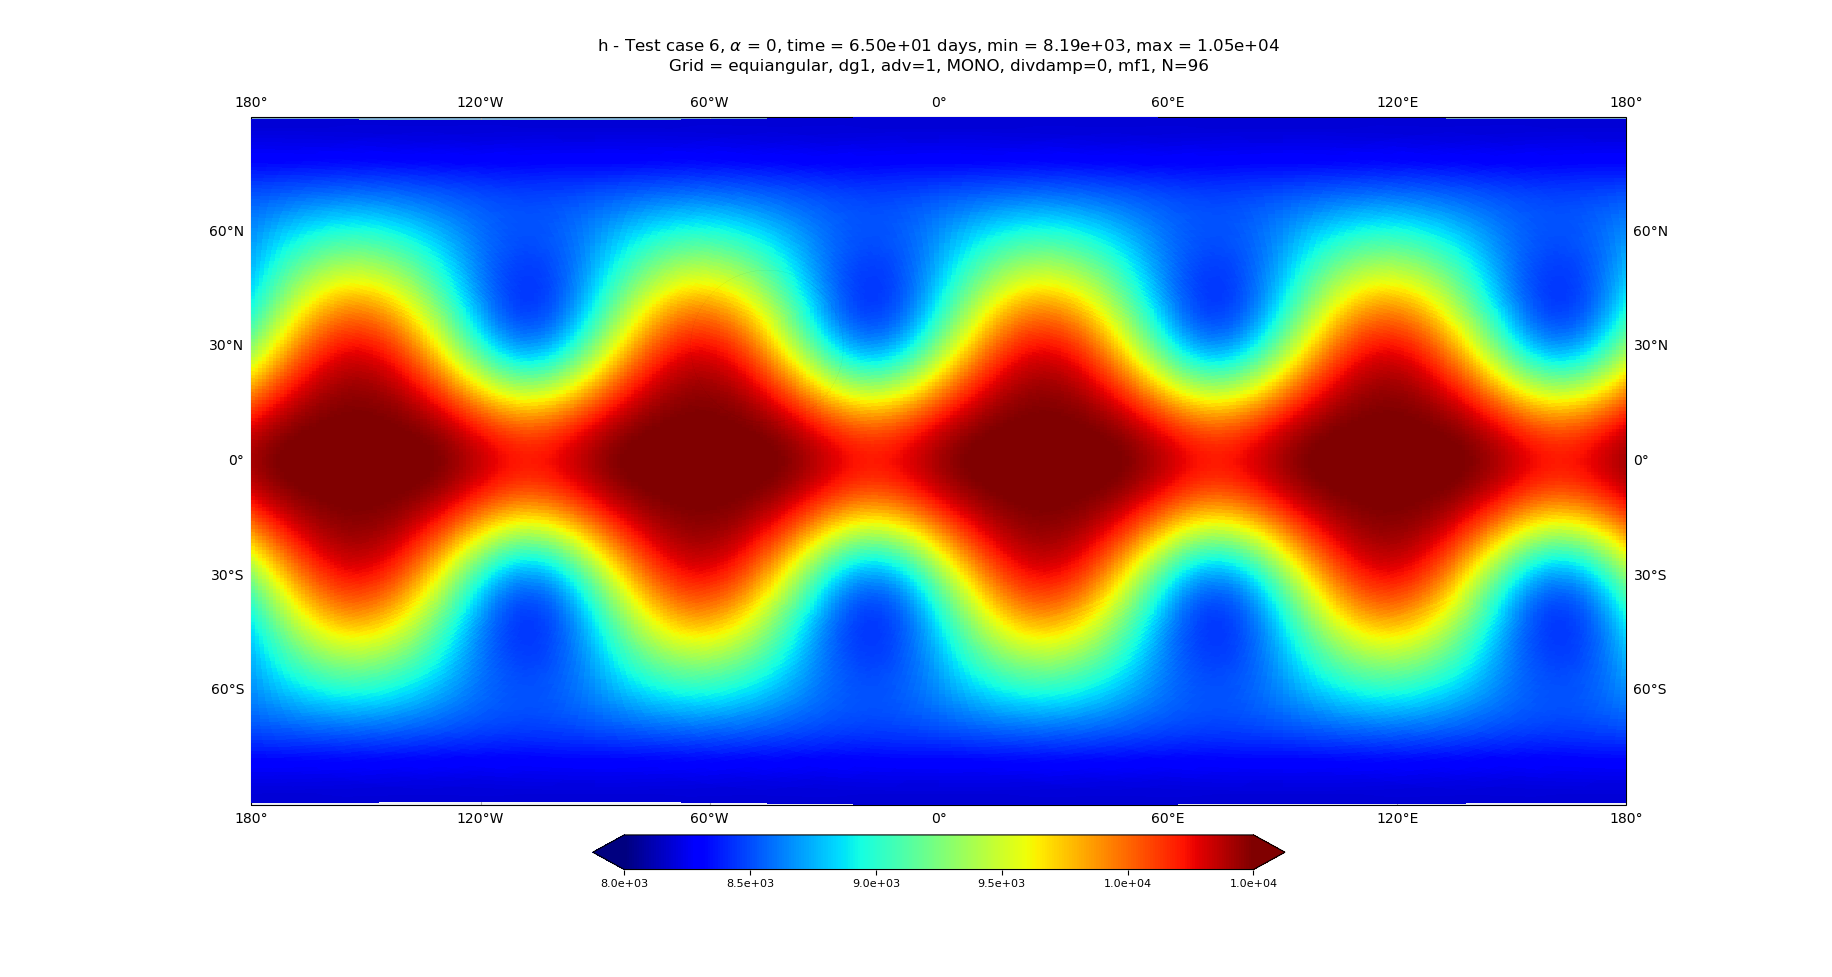
\includegraphics[width=1\linewidth]{h_tc6_t65_alpha0_C96_g2_dg1_adv1_hord8_dd0_mf1_tf105}
		\caption{PL at day 65.\label{sw-rossby-h-d65-pl}}
	\end{subfigure}
	
	\begin{subfigure}{0.49\textwidth}
		\centering
		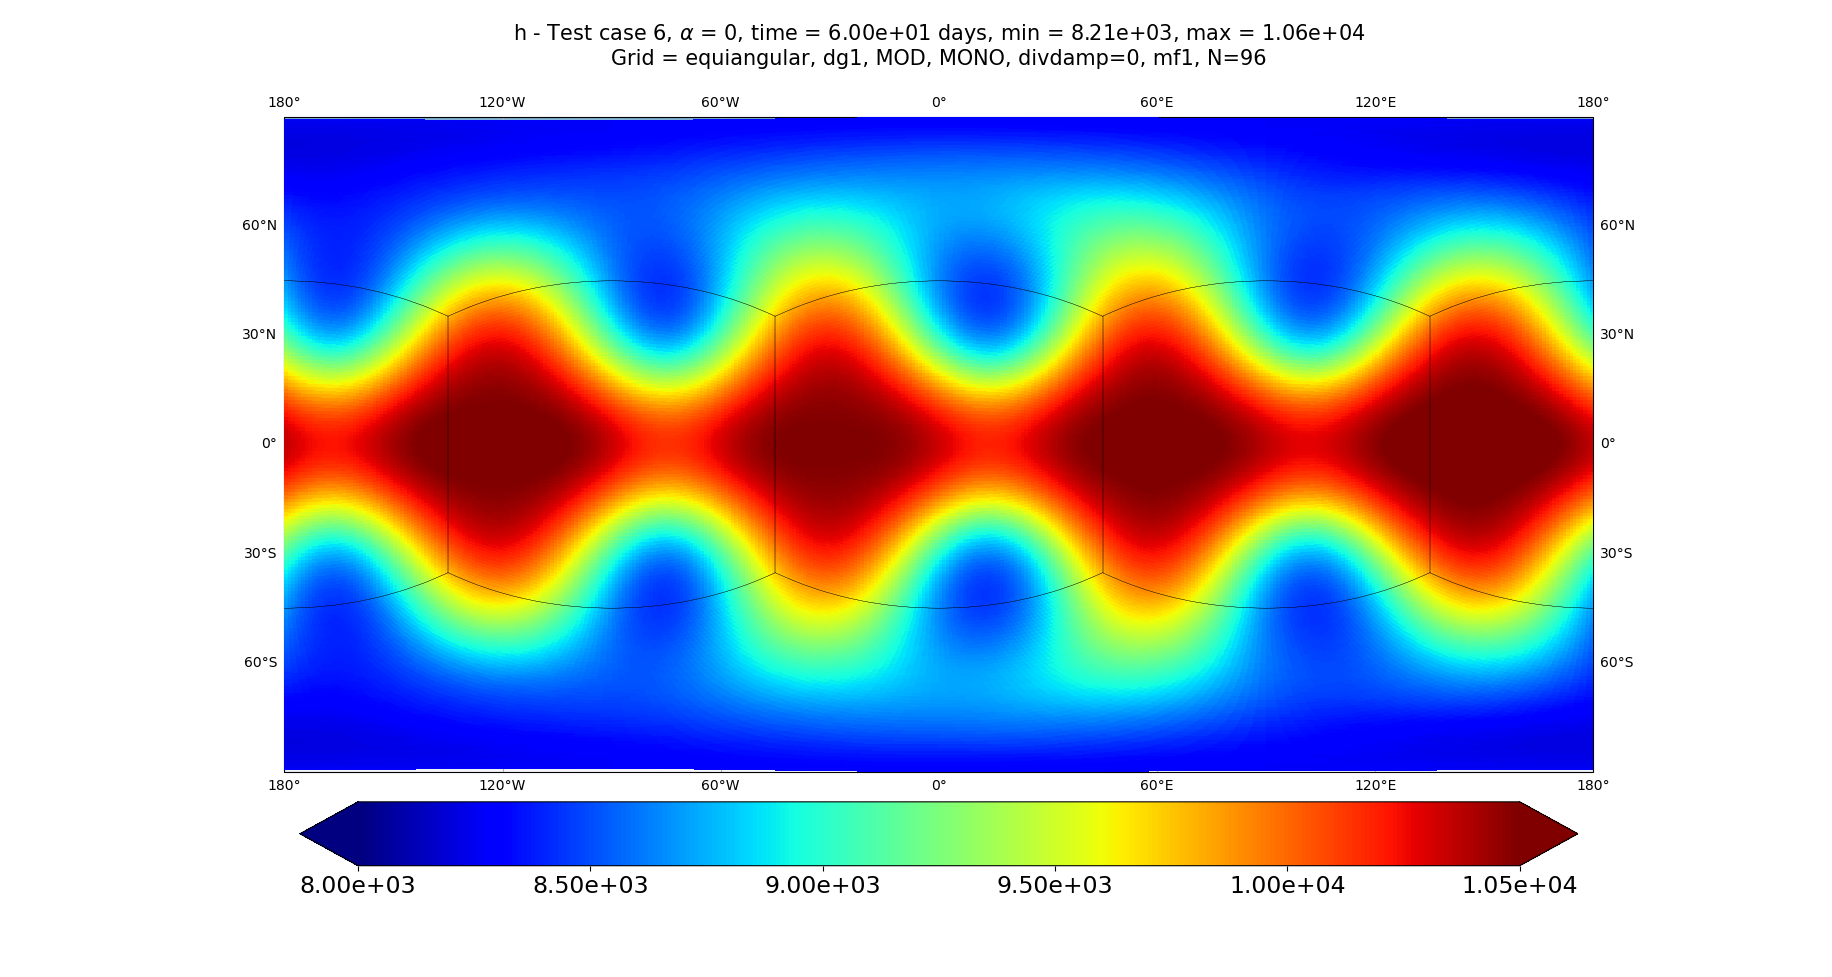
\includegraphics[width=1\linewidth]{h_tc6_t60_alpha0_C96_g2_dg1_adv2_hord8_dd0_mf1_tf105}
		\caption{LT at day 60.\label{sw-rossby-h-d60-lt}}
	\end{subfigure}
	\begin{subfigure}{0.49\textwidth}
		\centering
		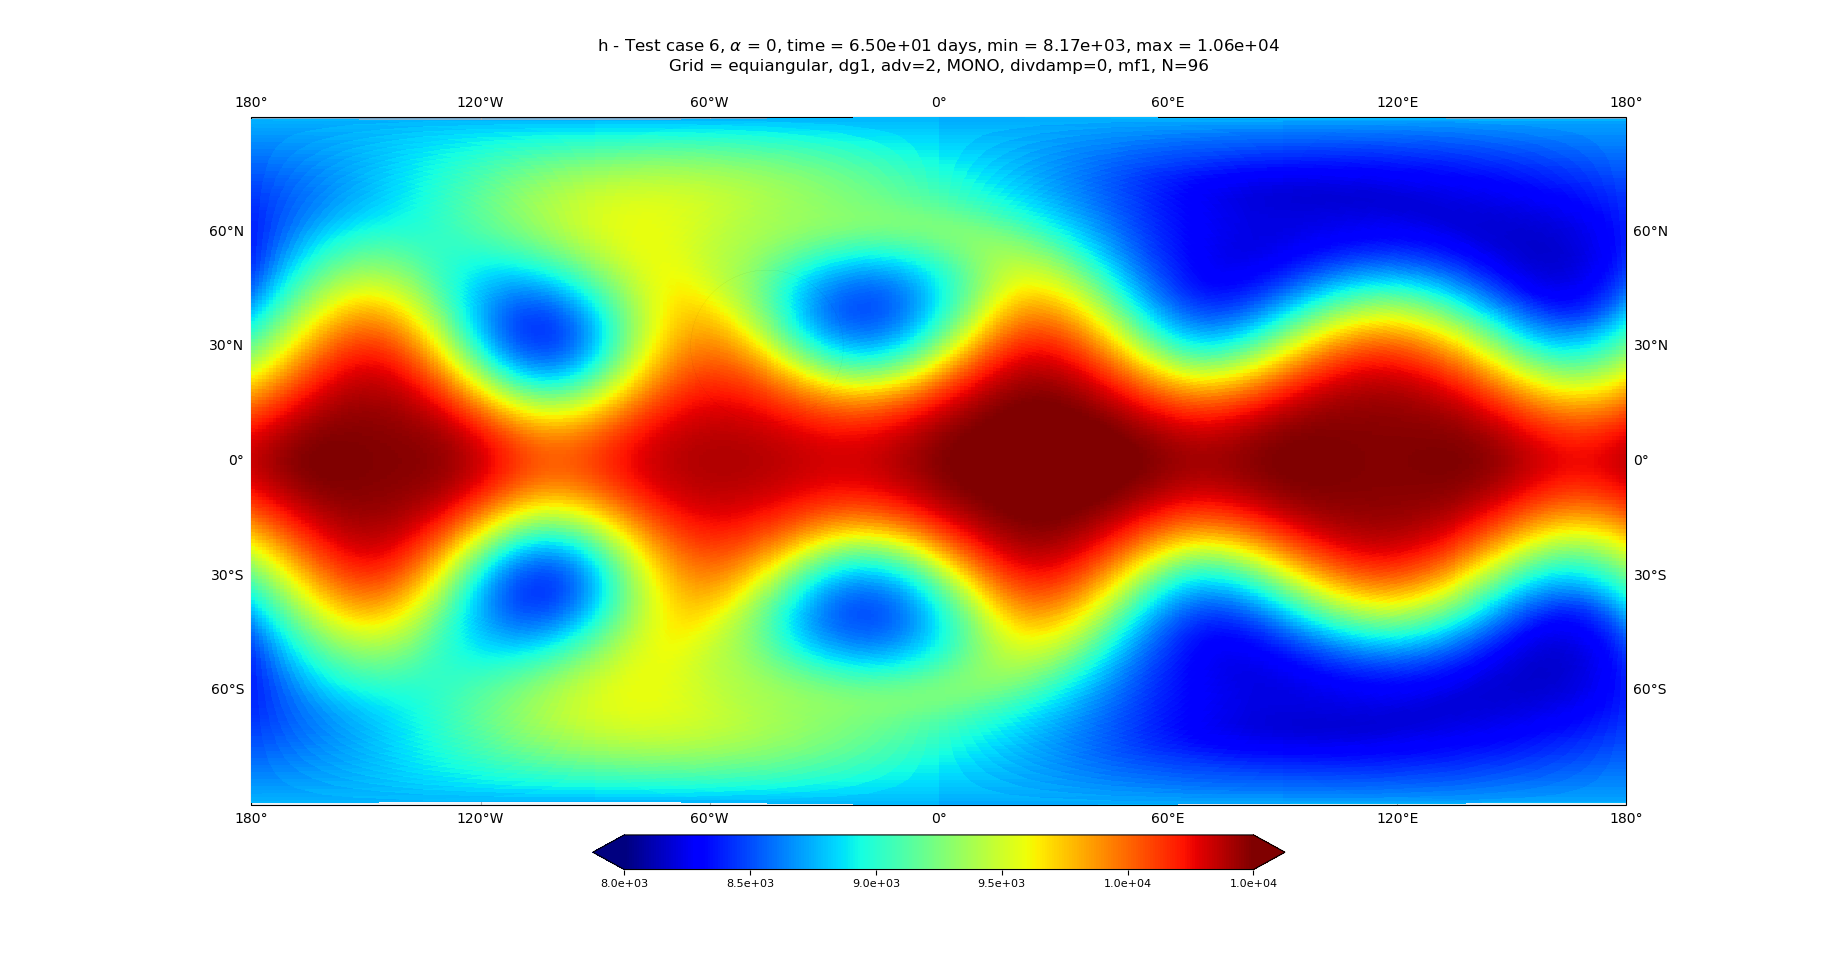
\includegraphics[width=1\linewidth]{h_tc6_t65_alpha0_C96_g2_dg1_adv2_hord8_dd0_mf1_tf105}
		\caption{LT at day 65.\label{sw-rossby-h-d65-lt}}
	\end{subfigure}
	\caption{Rossby-Haurwitz wave test case:
		Fluid depth on the equiangular grid, with $N=96$ and without divergence damping.
		PL scheme results are shown in (a) and (b) on days 60 and 65, respectively.
		LT scheme results are shown in (c) and (d) on days 60 and 65, respectively.
		\label{sw-rossby-h}}
\end{figure}
We ran this test for 100 days on the equi-edge and equiangular grids with $N=96$.
When we did not employ divergence damping, the results of the equi-edge grid became unstable for both schemes before day 60.
However, the equiangular grid could perform this test with divergence damping.
We show the wave shapes at days 60 and 65 in both schemes in Figure \ref{sw-rossby-h}, 
for the PL scheme (Figures \ref{sw-rossby-h-d60-pl} and \ref{sw-rossby-h-d65-pl}) and 
for the LT scheme (Figures \ref{sw-rossby-h-d60-lt} and \ref{sw-rossby-h-d65-lt}).
It is clear that the LT scheme can maintain the wave for 60 days, but the wave breaks at day 65. 
However, PL can preserve the shape of the wave for more than 65 days. 
In fact, it maintains the wave for approximately 100 days, as reported by \citet{mouallem:2023}.

When we use divergence damping, the equi-edge grid achieves numerical stability,
and we depict the wave in Figure \ref{sw-rossby-h-div-g0}.
We can see that the addition of divergence damping anticipates the wave break for the LT scheme,
which occurs at 55 days, as shown in Figures \ref{sw-rossby-h-d60-lt-div-g0} and \ref{sw-rossby-h-d65-lt-div-g0}. 
The PL scheme, again, maintains the wave (Figures \ref{sw-rossby-h-d60-pl-div-g0} and \ref{sw-rossby-h-d65-pl-div-g0}).
However, in this case, the wave breaks earlier as well, at approximately day 95 (not shown).
Similar results are observed for the equiangular grid with divergence damping and we will omit them here.

The PL ability to keep the wave for 100 days is remarkable.
The Rossby-Haurwitz wave is known for being a dynamically unstable test case, as investigated by \citet{thuburn:2000}. 
Although our scheme has reduced the wave shape, it is similar,
for instance, to the spectral model breaking time, as reported by \citet{thuburn:2000}, which is between 50 and 55 days.
\begin{figure}[!h]
	\centering
	\begin{subfigure}{0.48\textwidth}
		\centering
		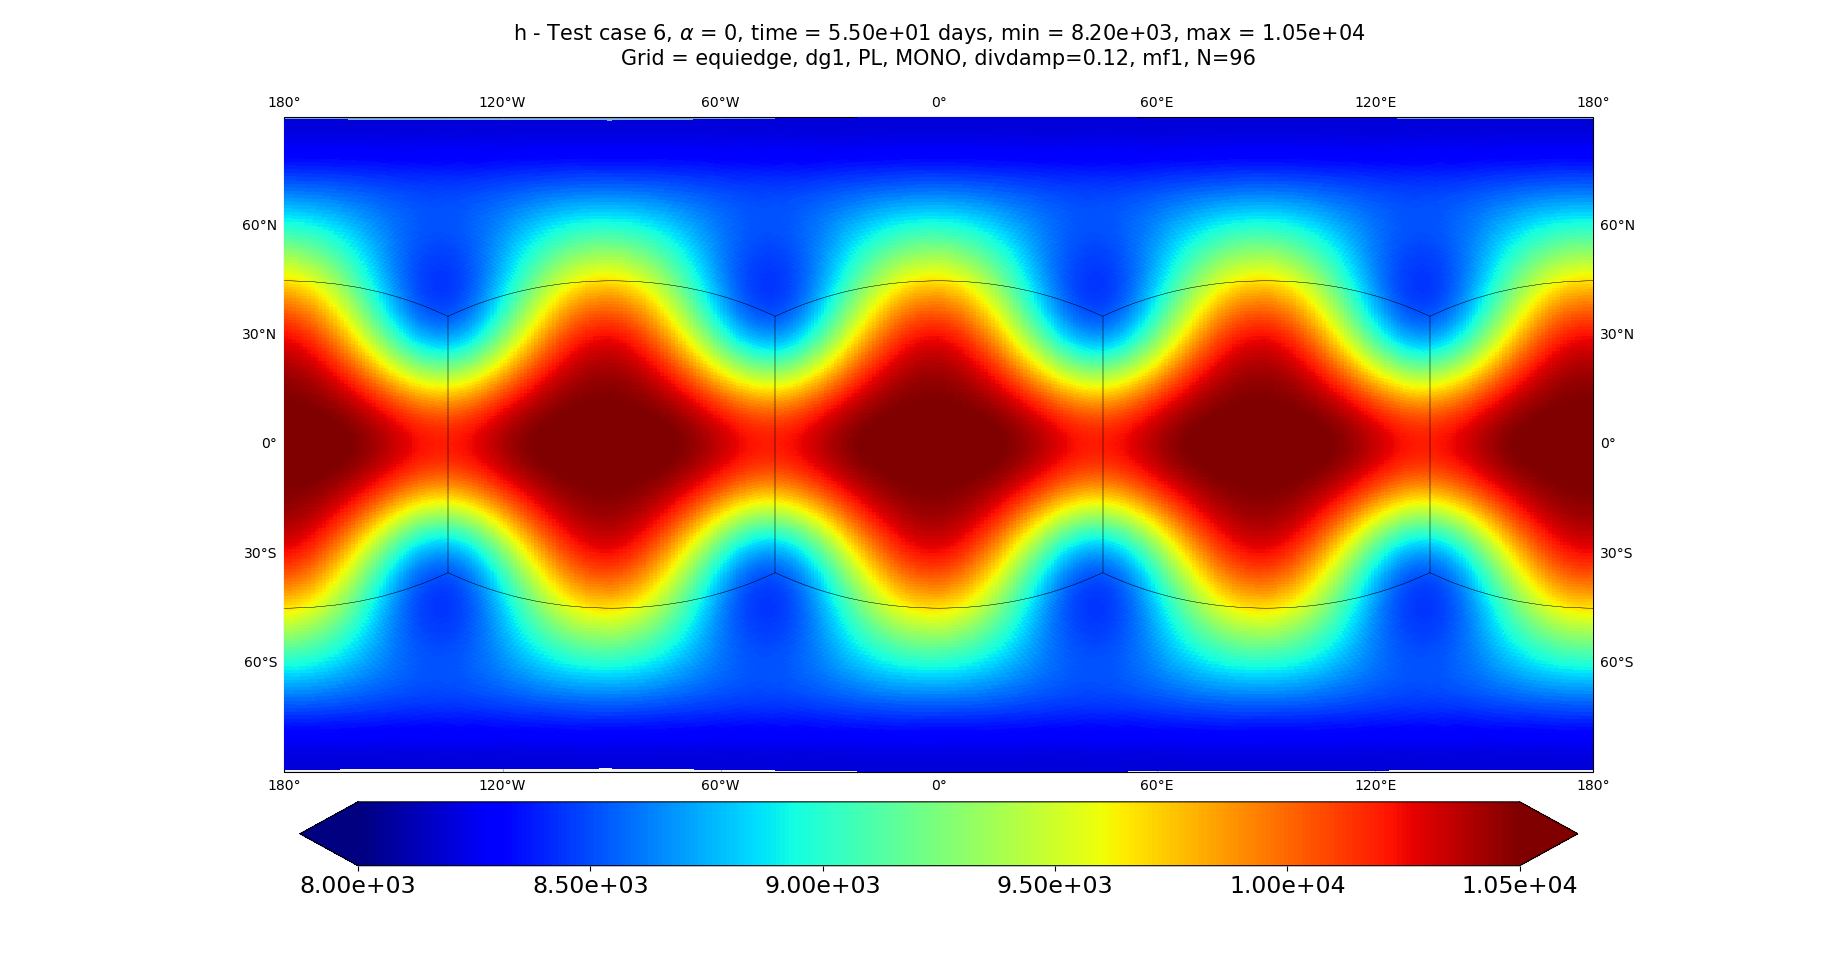
\includegraphics[width=1\linewidth]{h_tc6_t55_alpha0_C96_g0_dg1_adv1_hord8_dd0.12_mf1_tf105}
		\caption{PL at day 55.\label{sw-rossby-h-d60-pl-div-g0}}
	\end{subfigure}
	\begin{subfigure}{0.48\textwidth}
		\centering
		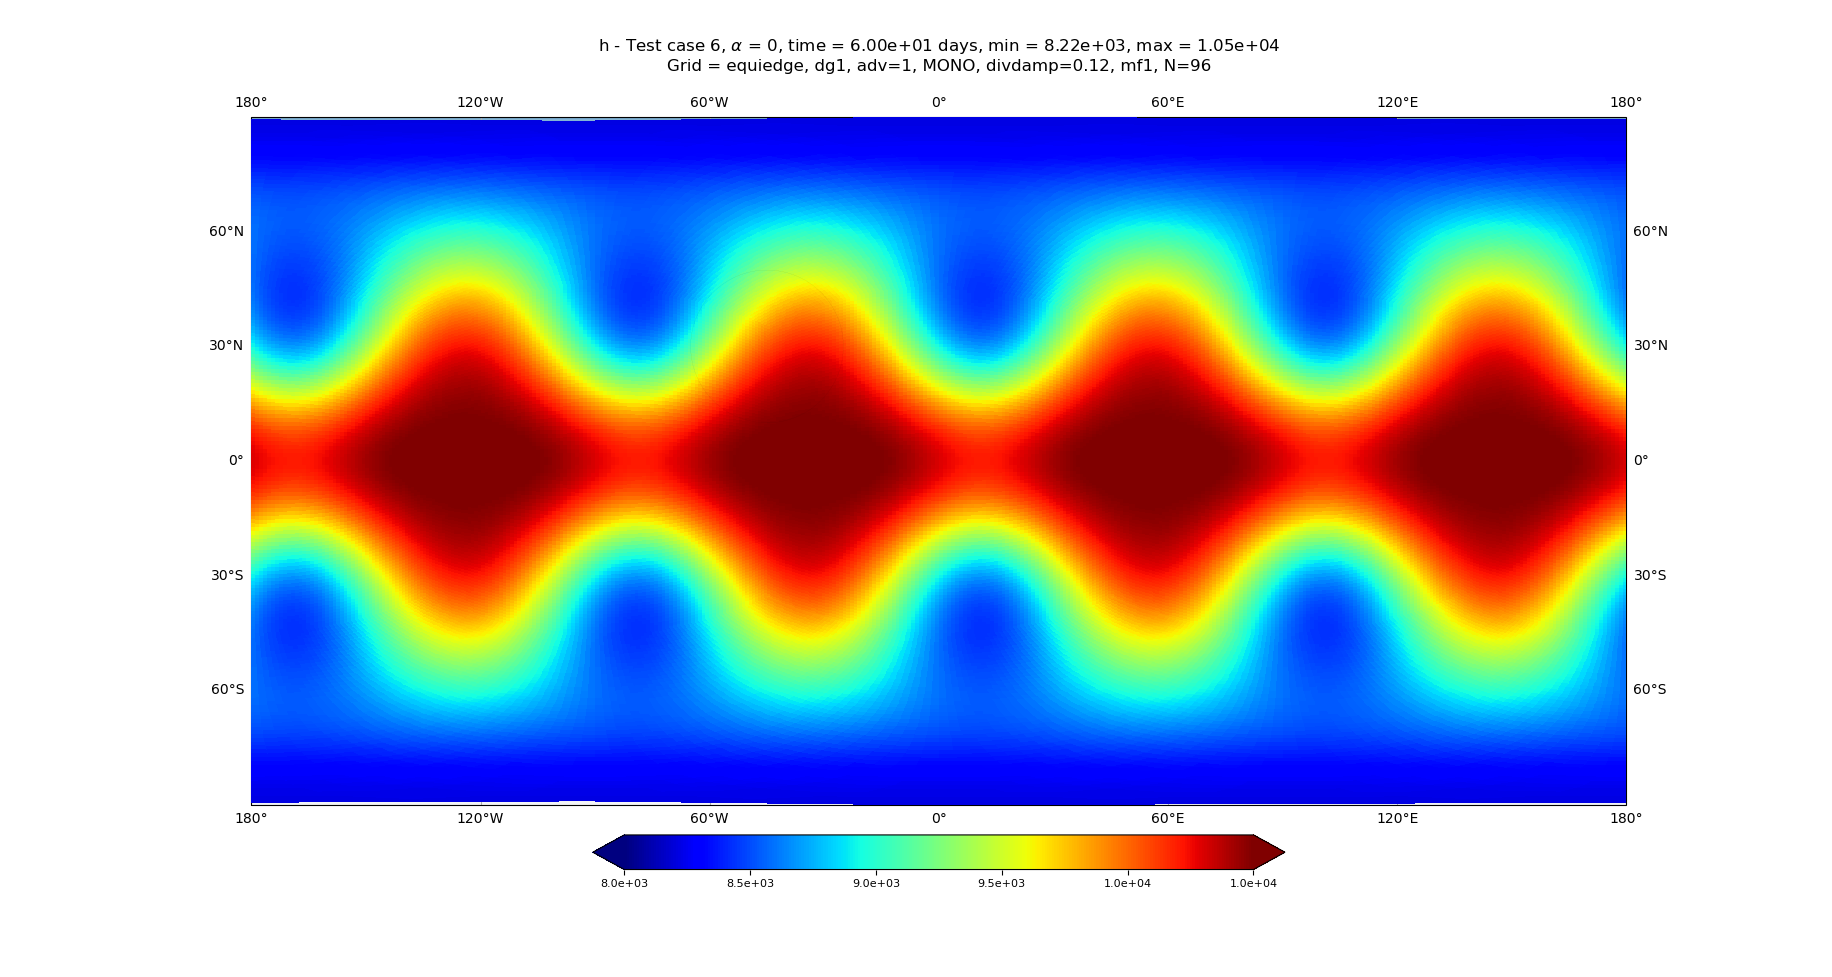
\includegraphics[width=1\linewidth]{h_tc6_t60_alpha0_C96_g0_dg1_adv1_hord8_dd0.12_mf1_tf105}
		\caption{PL at day 60.\label{sw-rossby-h-d65-pl-div-g0}}
	\end{subfigure}
	
	\begin{subfigure}{0.49\textwidth}
		\centering
		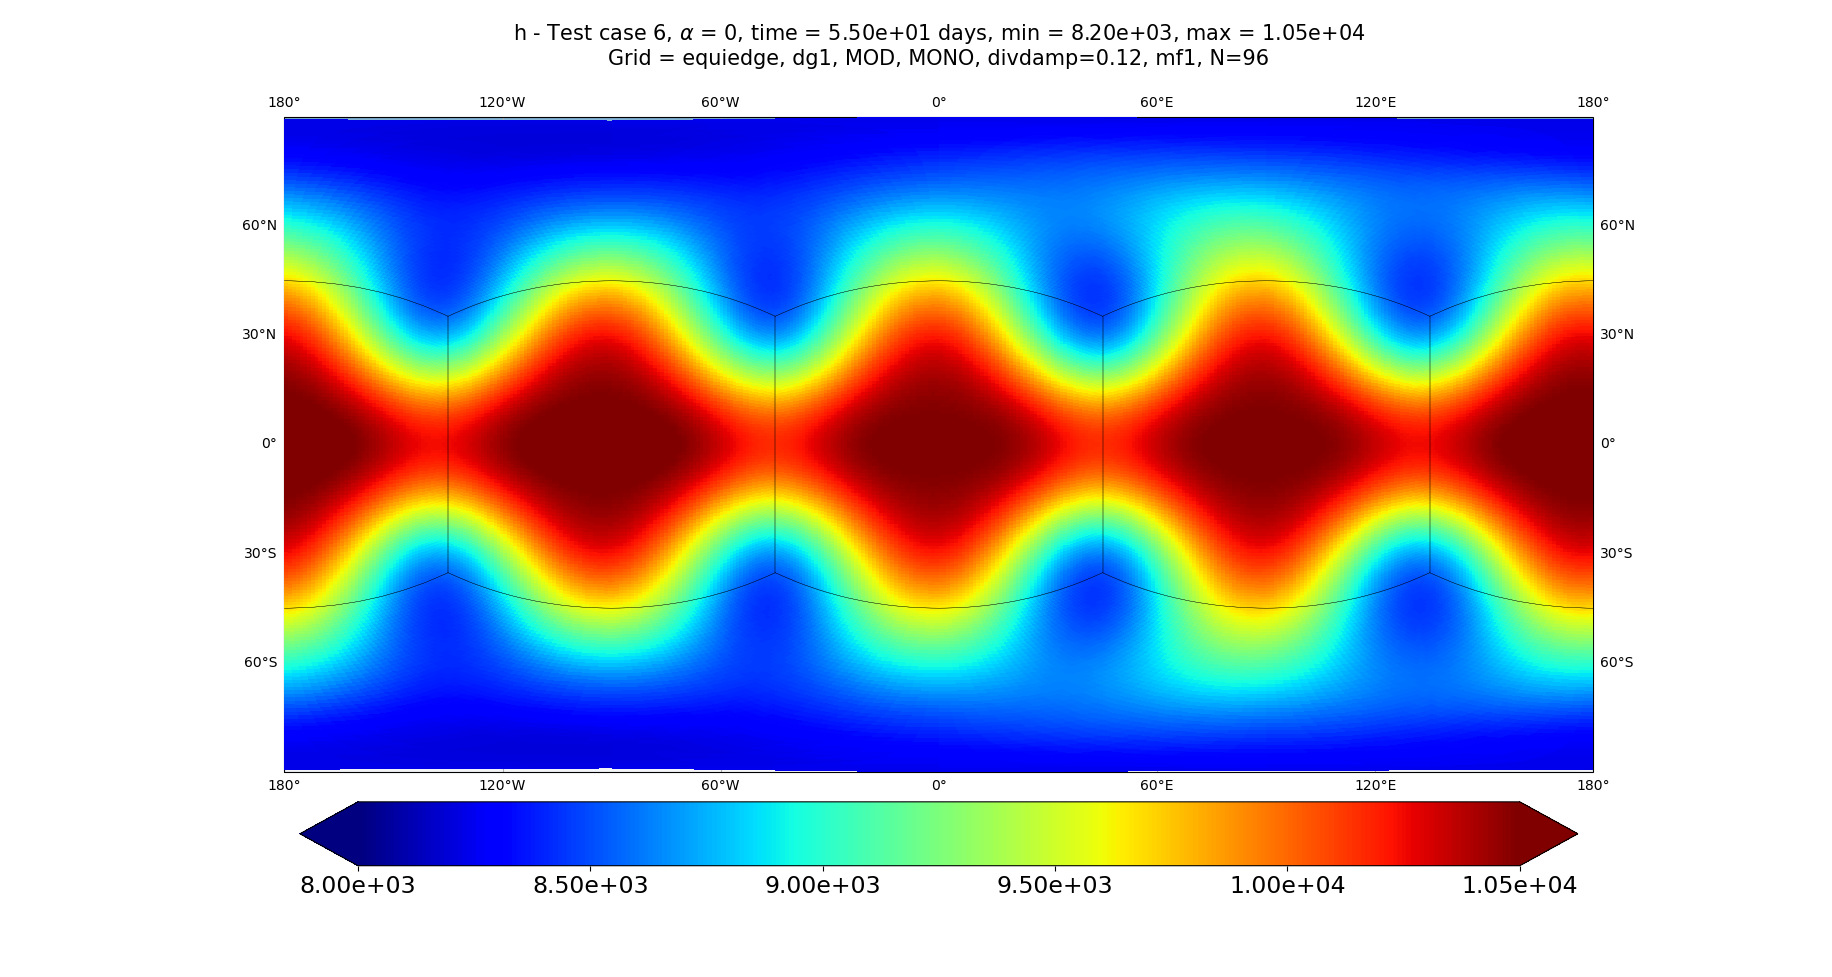
\includegraphics[width=1\linewidth]{h_tc6_t55_alpha0_C96_g0_dg1_adv2_hord8_dd0.12_mf1_tf105}
		\caption{LT at day 55.\label{sw-rossby-h-d60-lt-div-g0}}
	\end{subfigure}
	\begin{subfigure}{0.49\textwidth}
		\centering
		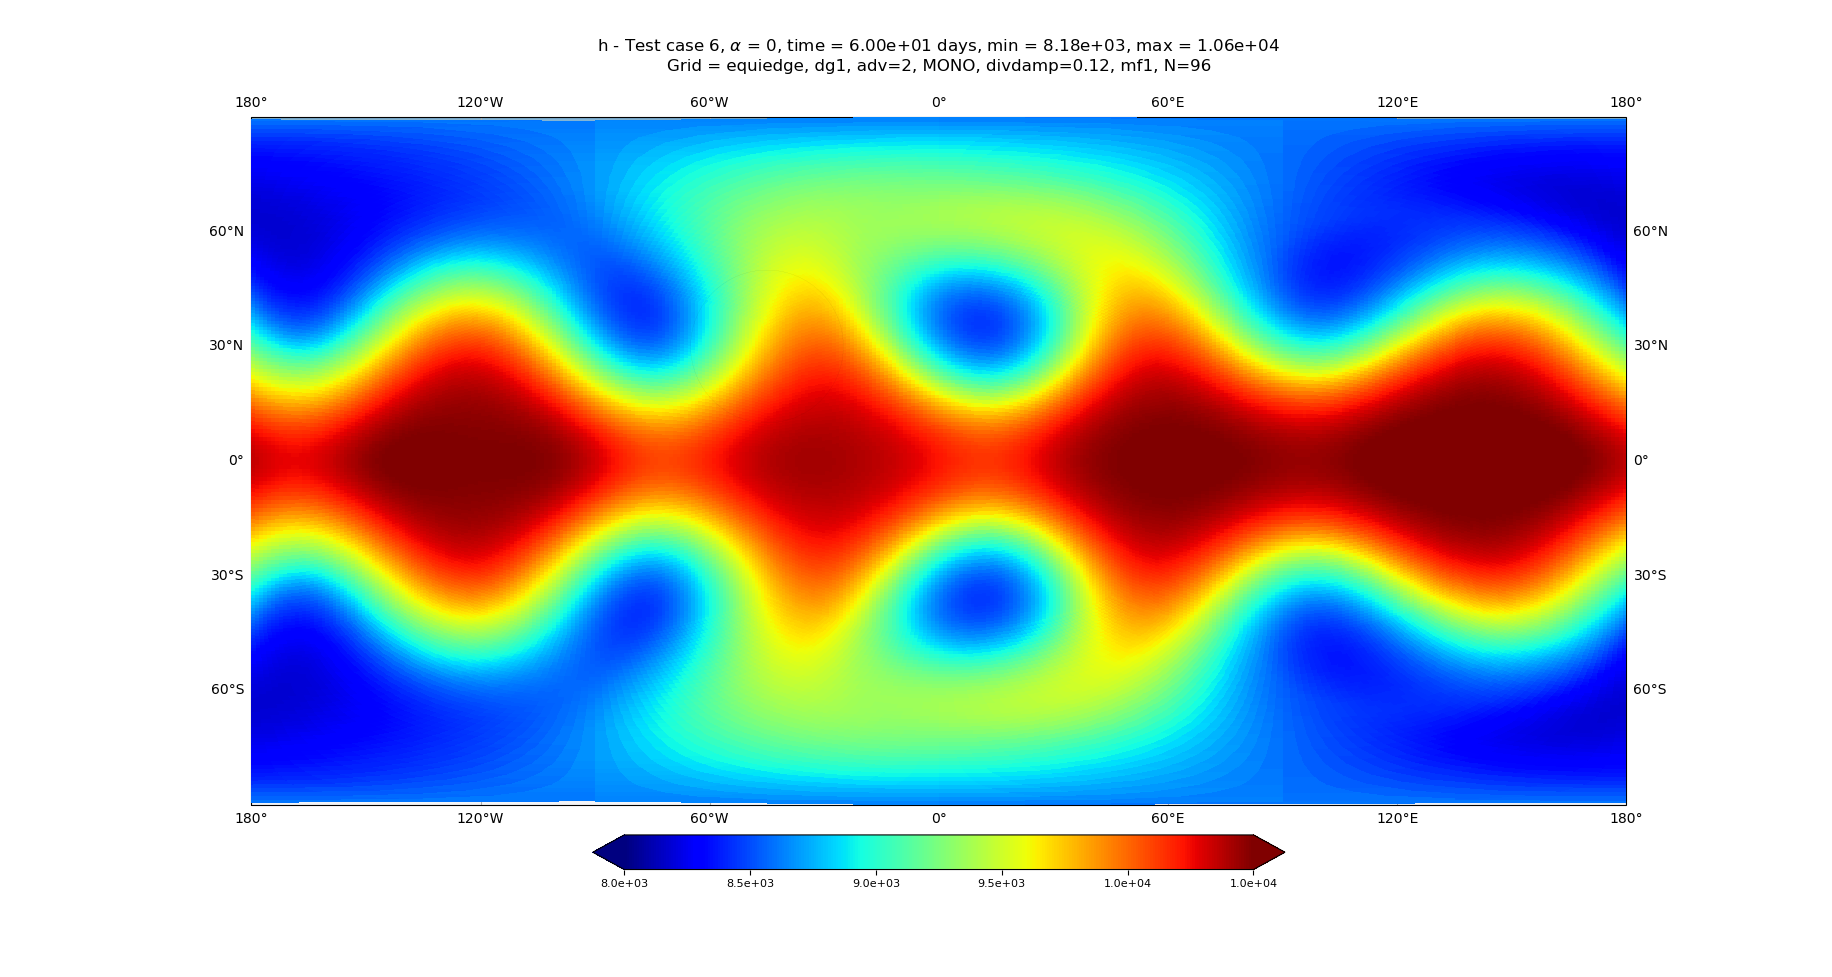
\includegraphics[width=1\linewidth]{h_tc6_t60_alpha0_C96_g0_dg1_adv2_hord8_dd0.12_mf1_tf105}
		\caption{LT at day 60.\label{sw-rossby-h-d65-lt-div-g0}}
	\end{subfigure}
	\caption{Rossby-Haurwitz wave test case:
		Fluid depth on the equi-edge grid, with $N=96$ and divergence damping.
		PL scheme results are shown in (a) and (b) on days 55 and 60, respectively.
		LT scheme results are shown in (c) and (d) on days 55 and 60, respectively.
		\label{sw-rossby-h-div-g0}}
\end{figure}






\newpage
%\subsection{Barotropically unstable jet with perturbation}
\section{Conclusions}
\label{sec:conclusions}
In this Chapter, we provided a detailed description of the FV3 shallow-water solver on the cubed-sphere. 
This solver begins with the shallow water equations written in the vector invariant form and considers their C and D-grid discretization.
We presented a general discretization of the shallow water equations on the C and D-grids and showed that they can be solved using finite-volume fluxes.
The C-grid solver is computed for a half time step, and the finite-volume fluxes use the classical upwind scheme, providing the winds centered at time.
This part of the scheme is designed to be computationally cheap.

Following that, the D-grid solver can use the time-centered winds from the C-grid solver and apply the PPM fluxes to update the fluid depth,
as well as absolute vorticity and kinetic energy fluxes. 
Then we discussed how our advection scheme from Chapter \ref{chp-cs-fv} can be used in the shallow-water solver. 
Since the C-grid is supposed to be computationally inexpensive and our scheme uses PPM, we decided to leave it unchanged. 
We consider our new finite-volume advection scheme to compute the fluid depth and the absolute vorticity fluxes on the D-grid.

We then ran the geostrophic balance flow test case for 5 days with and without divergence damping.
We observed that both advection schemes become numerically unstable for the equi-edge grid when no divergence damping is used,
which is not observed on the equiangular grid.
With divergence damping, both schemes are numerically stable on both grids.
Additionally, we noticed that our scheme helps to slightly reduce the $L_{\infty}$ errors when the scheme is numerically stable.
We analyzed the runtime and found that our advection scheme adds a very small additional computational burden.

\textcolor{black}{
We also analyzed the flow over a mountain test case and showed that our scheme yields very similar results to the current FV3 advection scheme.
Since this test case does not have an exact solution known, we have used the semi-Lagrangian semi-implicit shallow-water model ENDGame, 
which is used in the current operational UK Met Office dynamical core, as the reference solution.
Additionally, the equiangular grid managed to run this test without divergence damping,
while the equi-edge grid required divergence damping to run this test without creating large errors.}

\textcolor{black}{
The Rossby-Haurwitz wave test case was also investigated. 
The goal of this test is to assess the ability of a scheme to propagate the wave to the east and maintain the shape of the wave. 
However, this test is dynamically unstable and the wave eventually breaks. 
We showed that our scheme keeps the wave for 55-60 days, while the FV3 scheme keeps the wave for 95-100 days. 
Although we have reduced the wave breaking time, we pointed out that it is a little better than, for instance, the spectral model.}

The goal of this chapter was to describe the shallow-water solver, demonstrate how our scheme may be used and compare the computational performance.
However, a more comprehensive analysis of the shallow-water model using our scheme is certainly needed. 
We point out that most of the classical shallow-water tests available in the literature \citep{will:1992, galewsky:2004} have no or small divergence. 
Therefore, we expect that our scheme would introduce similar results in these tests because,
 as we have seen in Chapter \ref{chp-cs-fv}, our advection is slightly better for divergence-free winds and  significantly better only for divergent winds.
